\documentclass[12pt,oneside]{book}

\def\ShowSoln{0}


\usepackage[toc,page]{appendix}
\usepackage{marginnote}
\newcommand{\ds}{\displaystyle}
\newcommand{\bx}{{\bf x}}
\newcommand{\bw}{{\bf w}}
\newcommand{\bo}{{\bf 0}}
\newcommand{\bv}{{\bf v}}
\newcommand{\bu}{{\bf u}}
\newcommand{\bq}{{\bf q}}
\newcommand{\by}{{\bf y}}
\newcommand{\bb}{{\bf b}}
\newcommand{\ba}{{\bf a}}
\newcommand{\grad}{\boldsymbol{\nabla}}
% \newcommand{\bn}{\boldsymbol{n}}
\newcommand{\dd}[2]{\frac{d #1}{d #2}}
\newcommand{\ddd}[2]{\frac{d^2 #1}{d #2^2}}
\newcommand{\cc}{\mathbb{C}}
\newcommand{\rr}{\mathbb{R}}
\newcommand{\nn}{\mathbb{N}}
\newcommand{\qq}{\mathbb{Q}}
\newcommand{\zz}{\mathbb{Z}}
\newcommand{\lp}{\left(}
\newcommand{\rp}{\right)}
\newcommand{\lb}{\left[}
\newcommand{\rb}{\right]}
\newcommand{\andd}[1]{\quad\text{and}\quad}
\newcommand{\orr}[1]{\quad\text{or}\quad}
\newcommand{\forr}[1]{\quad\text{for}\quad}
\newcommand{\st}[1]{\quad\text{such that}\quad}
\newcommand{\conj}[1]{\quad\text{#1}\quad}
\newcommand{\ra}{\quad\Rightarrow\quad}
\newcommand{\pd}[2]{\frac{\partial #1}{\partial #2}}
\newcommand{\pdd}[2]{\frac{\partial^2 #1}{\partial #2^2}}
\newcommand{\pddm}[3]{\frac{\partial^2 #1}{\partial #2 \partial #3}}
\newcommand{\deriv}[2]{\frac{d #1}{d #2}}
\renewcommand{\Re}{\mathbb{R}}
\newcommand{\lap}[1]{\mathcal{L}\left\{ #1 \right\}}
\newcommand{\lapinv}[1]{\mathcal{L}^{-1}\left\{ #1 \right\}}

\usepackage[scale=2]{ccicons}
\usepackage{enumitem}
\usepackage{multicol}
\usepackage[labelsep=period]{caption}
\usepackage{tabu}
% \usepackage{pdiag}
\usepackage[table]{xcolor}
\usepackage{tikz}
\usetikzlibrary{arrows,automata,positioning}
\usetikzlibrary{patterns,decorations}
\usepackage{pgfplots}
\pgfplotsset{compat=1.13}
\usepackage{rotating}
\usepackage[notextcomp]{kpfonts} 
\usepackage{graphicx}
\usepackage{eurosym}
\usepackage{amsfonts}
\usepackage{amsmath}
\usepackage{amssymb}
\usepackage{amsthm}
\usepackage{stmaryrd}
\usepackage{wasysym}
\usepackage{amsthm}
\usepackage[margin=1in]{geometry}
\geometry{headheight=12pt}
\usepackage[hang,flushmargin,symbol*]{footmisc}
\usepackage{color}
\definecolor{darkblue}{rgb}{0, 0, .6}
\definecolor{grey}{rgb}{.7, .7, .7}
\usepackage[breaklinks]{hyperref}
\usepackage[framed,numbered]{mcode}
\hypersetup{
	colorlinks=true,
	linkcolor=darkblue,
	anchorcolor=darkblue,
	citecolor=darkblue,
	urlcolor=darkblue,
	pdftitle={},
	pdfauthor={}
}

\tikzset{declare function={y(\x)=4-\x^2;},
plot fill/.style={fill=purple!75},
plot/.style={draw=black!80, thick},
bar/.style={fill=cyan, draw=white, thick},
marking/.style={fill=cyan!50!black, draw=cyan!50!black},
axis/.style={thick, draw=black!65, stealth-stealth}
      }

\usepackage{fancyhdr}
\pagestyle{fancy}
\lhead{\leftmark}
\chead{}
\rhead{\thepage \ifnum\ShowSoln=1 {\color{red} {\bf Solutions}} \fi}
\lfoot{
\includegraphics[width=1.5cm]{CreativeCommons.png}}
\cfoot{}
\rfoot{}
% \setlength{\headheight}{12pt}
\theoremstyle{definition}
\newtheorem{theorem}{Theorem}[chapter]
\newtheorem{acknowledgement}[theorem]{Acknowledgement}
% \newtheorem{algorithm}[theorem]{Algorithm}
\newtheorem{axiom}[theorem]{Axiom}
\newtheorem{case}[theorem]{Case}
\newtheorem{claim}[theorem]{Claim}
\newtheorem{conclusion}[theorem]{Conclusion}
\newtheorem{condition}[theorem]{Condition}
\newtheorem{conjecture}[theorem]{Conjecture}
\newtheorem{corollary}[theorem]{Corollary}
\newtheorem{criterion}[theorem]{Criterion}
% \newtheorem{definition}[theorem]{Definition}
% \newtheorem{example}[theorem]{Example}
\newtheorem{exercise}[theorem]{Exercise}
\newtheorem{journal}[theorem]{Journal}
\newtheorem{lemma}[theorem]{Lemma}
\newtheorem{notation}[theorem]{Notation}
\newtheorem{prob}[theorem]{Problem}
\newtheorem{chal}[theorem]{Challenge}
% \newtheorem{problem}[theorem]{Problem}
\newtheorem{proposition}[theorem]{Proposition}
\newtheorem{remark}[theorem]{Remark}
\newtheorem{summary}[theorem]{Summary}
\newtheorem{skeleton}[theorem]{Skeleton Proof}
\newtheorem{activity}[theorem]{Activity}
\newtheorem{intuitivedef}[theorem]{Intuitive Definition}

\newenvironment{problem}{\begin{prob}}{\hfill$\blacktriangle$\end{prob}}
\newenvironment{challenge}{\begin{chal}}{\hfill$\blacktriangle$\end{chal}}

\usepackage{silence}
\usepackage{mdframed}
\WarningFilter{mdframed}{You got a bad break}
\WarningFilter{Fancyhdr}{\headheight is too small (12.0pt)}

\newtheorem{defn}[theorem]{Definition}
\newenvironment{definition}
{\begin{mdframed}[backgroundcolor=blue!15]\begin{defn}}
        {\end{defn}\end{mdframed}}

\newenvironment{thm}
{\begin{mdframed}[backgroundcolor=red!15]\begin{theorem}}
        {\end{theorem}\end{mdframed}}
\newenvironment{cor}
{\begin{mdframed}[backgroundcolor=red!15]\begin{corollary}}
        {\end{corollary}\end{mdframed}}

\newtheorem{tchnq}[theorem]{Technique}
\newenvironment{technique}
{\begin{mdframed}[backgroundcolor=green!10]\begin{tchnq}}
        {\end{tchnq}\end{mdframed}}

\newtheorem{alg}[theorem]{Algorithm}
\newenvironment{algorithm}
{\begin{mdframed}[backgroundcolor=green!10]\begin{alg}}
        {\end{alg}\end{mdframed}}

\newtheorem{ex}[theorem]{Example}
\newenvironment{example}
{\begin{mdframed}[backgroundcolor=black!10]\begin{ex}}
        {\end{ex}\end{mdframed}}


\newtheorem{homework}[theorem]{Homework Exercise}


\newsavebox{\savepar}
\newenvironment{textbox}{\noindent\begin{lrbox}{\savepar}\begin{minipage}[c]{.98\textwidth}}{\end{minipage}\end{lrbox}\fcolorbox{black}{white}{\usebox{\savepar}}}


\newcommand{\solution}[1]{\ifnum\ShowSoln=1 {\color{red} {\bf Solution:} #1}\fi}
\newcommand{\hint}[1]{\ifnum\ShowSoln=1 {\color{blue} {\bf Hint:} #1}\fi}
\newcommand{\teacher}[1]{\ifnum\ShowSoln=1 {\color{blue} {\bf Teacher Note:} #1}\fi}

\usetikzlibrary{shapes.geometric, arrows}

\tikzstyle{boxy} = [rectangle, rounded corners, minimum width=3cm, minimum
height=1cm,text centered, draw=black, fill=green!30]
\tikzstyle{boxysoln} = [rectangle, rounded corners, minimum width=3cm, minimum
height=1cm,text centered, draw=black, fill=red!30]
\tikzstyle{arrow} = [thick,->,>=stealth]
\tikzstyle{arrowdashed} = [thick,dashed,->,>=stealth]
\title{Numerical Methods \\ An Inquiry-Based Approach
    \ifnum\ShowSoln=1 {\color{red} \\ {\bf Solutions}} \fi}
\date{Content Last Updated: \today}
\author{
%     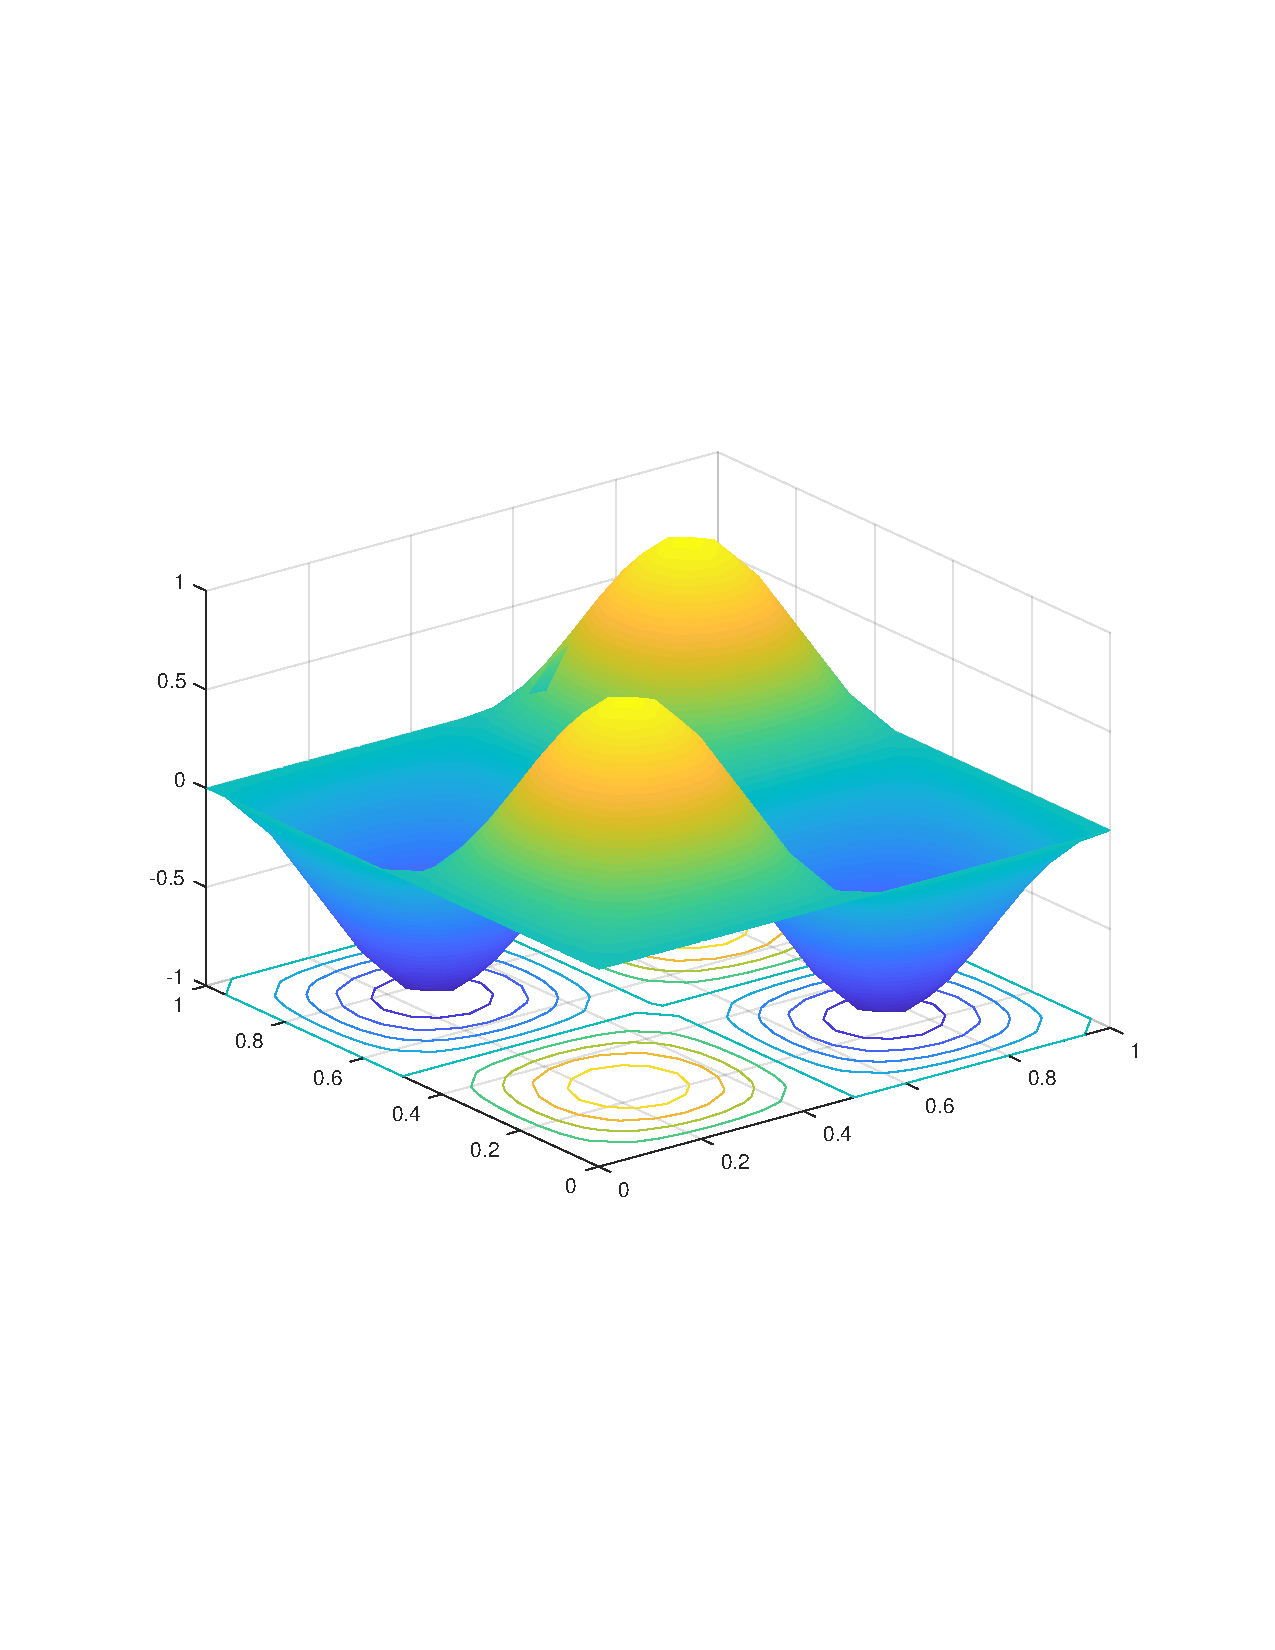
\includegraphics[width=0.6\columnwidth, trim=0cm 6cm 0cm 8cm,
% clip=true]{CoverWave.pdf} \\
Eric Sullivan \\ Department of
Mathematics \\
Carroll College, Helena, MT \\ \texttt{esullivan@carroll.edu} \\
%     This work is licensed under
%     \href{https://creativecommons.org/licenses/by-nc-sa/4.0/}{Creative Commons:
%     NonCommercial-ShareAlike}\\
% 

\includegraphics{CreativeCommons.png} % \\\vspace{3in}
}

\begin{document}
\maketitle
% \html{<a rel=``license'' href=``http://creativecommons.org/licenses/by-nc-sa/4.0/''><img
%     alt=``Creative Commons License'' style=``border-width:0''
%     src=``https://i.creativecommons.org/l/by-nc-sa/4.0/88x31.png'' /></a><br /><span
%     xmlns:dct=``http://purl.org/dc/terms/'' href=``http://purl.org/dc/dcmitype/Text''
%     property=``dct:title'' rel=``dct:type''>Differential Equations and Linear
%     Algebra</span> by <span xmlns:cc=``http://creativecommons.org/ns#''
%     property=``cc:attributionName''>Eric R. Sullivan</span> is licensed under a <a
%     rel=``license'' href=``http://creativecommons.org/licenses/by-nc-sa/4.0/''>Creative
% Commons Attribution-NonCommercial-ShareAlike 4.0 International License</a>.}
% \vspace{0.2in}
\newpage
\noindent \copyright Eric Sullivan. Some Rights Reserved.

\vspace{0.2in}
This work is licensed under a Creative Commons Attribution-NonCommercial-ShareAlike 4.0
International License.
You may copy, distribute, display, remix, rework, and perform this copyrighted work, but only if
you give credit to Eric Sullivan, and all derivative works based upon it must be published
under the Creative Commons Attribution-NonCommercial-Share Alike 4.0 United States License. Please
attribute this work to Eric Sullivan, Mathematics Faculty at Carroll College,
esullivan@carroll.edu. To view a copy of this license, visit\\
\href{https://creativecommons.org/licenses/by-nc-sa/4.0/}{https://creativecommons.org/licenses/by-nc-sa/4.0/}\\
or send a letter to Creative Commons, 171 Second Street, Suite 300, San Francisco,
California, 94105, USA.
\tableofcontents


% \setcounter{chapter}{-1}
\frontmatter
\chapter{Preface}
This book grew out of lecture notes, classroom activities, code, examples, exercises,
projects, and challenge problems for my introductory course on
numerical methods.  The prerequisites for this material include a firm understanding of
single variable calculus (though multivariable calculus doesn't hurt), a good
understanding of the basics of linear algebra, a good understanding of the basics of
differential equations, and some exposure to scientific computing (as seen in other math
classes or perhaps from a computer science class). The primary audience is any
undergraduate STEM major with an interest in using computing to solve problems.

A note on the book's title: I do not call these materials ``numerical
analysis'' even though that is often what this course is called.  In these materials I
emphasize ``methods'' and implementation over rigorous mathematical ``analysis.''  While
this may just be semantics I feel that it is important to point out.  If you are looking
for a book that contains all of the derivations and rigorous proofs of the primary results
in elementary numerical analysis, then this not the book for you.  I have
intentionally written this material with an inquiry-based emphasis which means that this
is not a traditional text on numerical analysis -- there are plenty of those on the market
and I cite several wonderful traditional texts in the bibliography at the end of this
book.

\section{To The Student}

\subsection{The Inquiry-Based Approach}
% The inquiry-based approach can by summarized by one quote:
\begin{quote}
    {\it Any creative endeavor is built on the ash heap of failures.}
\end{quote}
% The material in this book is meant to make you think, build, construct, fail, struggle,
% and ultimately succeed in learning numerical methods.

\begin{problem}[Setting The Stage]
    Let's start the book off right away with a problem designed for groups, discussion,
    disagreement, and deep critical thinking.  This problem is inspired by Dana Ernst's
    first day IBL activity titled: \href{http://danaernst.com/setting-the-stage/}{Setting
    the Stage}.
    \begin{itemize}
        \item Get in groups of size 3-4.
        \item Group members should introduce themselves.
        \item For each of the questions that follow I will ask you to:
            \begin{enumerate}
                \item {\bf Think} about a possible answer on your own
                \item {\bf Discuss} your answers with the rest of the group
                \item {\bf Share} a summary of each group's discussion
            \end{enumerate}
    \end{itemize}
    {\bf Questions:} 
    \begin{description}
        \item[Question \#1:] What are the goals of a university education?
        \item[Question \#2:] How does a person learn something new?
        \item[Question \#3:] What do you reasonably expect to remember from your courses
            in 20 years?
        \item[Question \#4:] What is the value of making mistakes in the learning process?
        \item[Question \#5:] How do we create a safe environment where risk taking is
            encouraged and productive failure is valued?
    \end{description}
\end{problem}


This material is written with an Inquiry-Based Learning (IBL) flavor. In that sense, this
document could be used as a stand-alone set of materials for the course but these notes
are not a {\it traditional textbook} containing all of the expected theorems, proofs,
code, examples, and exposition. You are encouraged to work through problems and homework,
present your findings, and work together when appropriate. You will find that this
document contains collections of problems with only minimal interweaving exposition.  It
is expected that you do every one of the problems and then only use other more traditional
texts (or Google) as a backup when you are completely stuck.  Let me say that again: this
is not the only set of material for the course.  Your brain, your peers, and the books
linked in the next section are your best resources when you are stuck.

To learn more about IBL go to
\href{http://www.inquirybasedlearning.org/about/}{http://www.inquirybasedlearning.org/about/}.
The long and short of it is that you, the student, are the one that is doing the
work; proving theorems, writing code, working problems, leading discussions, and pushing
the pace. The instructor acts as a guide who only steps in to redirect conversations or to
provide necessary insight. 

You have the following jobs as a student in this class:
\begin{enumerate}
    \item {\bf Fight!}  You will have to fight hard to work through this material.  The fight is
        exactly what we're after since it is ultimately what leads to innovative thinking.
    \item {\bf Screw Up!}  More accurately, don't be afraid to screw up.  You should write code,
    work problems, and prove theorems then be completely unafraid to scrap what you've
    done and redo it from scratch.  Learning this material is most definitely a non-linear
    path.
\item {\bf Collaborate!}  You should collaborate with your peers with the following caveats:
    \begin{enumerate}
        \item When you are done collaborating you should go your separate ways.  When you
            write your solution you should have no written (or digital) record of your
            collaboration.  
        \item \underline{The internet is not a collaborator}.  Use of the internet to help
            solve these problems robs you of the most important part of this class; the
            chance for original thought.
    \end{enumerate}
\item {\bf Enjoy!}  Part of the fun of IBL is that you get to experience what it is like to
        think like a true mathematician / scientist.  It takes hard work but ultimately
        this should be fun!
\end{enumerate}

\subsection{Online Texts and Other Resources}\label{pref:resources}
If you are looking for online textbooks for numerical methods or numerical analysis I can
point you to a few of my favorites.  Some of the following online resources may be a good
place to help you when you're stuck but they will definitely say things a bit differently.
Use these resources wisely.
\begin{itemize}
    \item Holistic Numerical Methods
        \href{http://nm.mathforcollege.com/}{http://nm.mathforcollege.com/}\\
        The Holistic Numerical Methods book is probably the most complete free reference
        that I've found on the web.  This should be your source to look up deeper
        explanations of problems, algorithms, and code.
    \item Scientific Computing with MATLAB
        \href{http://gribblelab.org/scicomp/scicomp.pdf}{http://gribblelab.org/scicomp/scicomp.pdf}
    \item Tea Time Numerical Analysis
        \href{http://lqbrin.github.io/tea-time-numerical/}{http://lqbrin.github.io/tea-time-numerical/}
\end{itemize}


\section{To the Instructor}
If you are an instructor wishing to use these materials then I only ask that you adhere to the
Creative Commons license.  You are welcome to use, distribute, and remix these materials
for your own purposes.  Thanks for considering my materials for your course!  Let me know
if you have questions, edits, or suggestions: esullivan@carroll.edu.

\subsection{The Inquiry-Based Approach}
I have written these materials with an inquiry-based flavor.  This means that this is not
a traditional textbook.  I don't
lecture through hardly any of the material in the book.  Instead my classes are structured
so that students are given problems to work before class, we build off of those problems
in class, and we repeat.  The exercises at the end of the chapters are assigned weekly and
graded with a revision process in mind -- students redo problems if the coding was
incorrect, if the mathematics was incorrect, or if they somehow missed the point.  The
students are tasked with building most of the algorithms, code, intuition, and analysis
with my intervention only if I deem it necessary. 

Several of the problems throughout the book are meant to be done in groups either at
the boards in the classroom or in some way where they can share their work.  Much of my
class time is spent with students actively building algorithms or group coding.  The
beauty, as I see it, of IBL is that you can run your course in any way that is comfortable
for you.  You can lecture through some of the material in a more traditional way, you can
let the students completely discover some of the methods, or you can do a mix of both.

You will find that I do not give rigorous (in the mathematical sense) proofs or
derivations of many of the algorithms in this book.  I tend to lean on
numerical experiments to allow students to discover algorithms, error estimates, and other
results without the rigor.
The makeup of my classes tends to be math majors along with engineering, computer science,
physics, and data science students.  While the math majors need to eventually see the
rigorous derivations the other majors, I think, are better served working from an
experimental approach rather than a theorem-proof approach.

\subsection{The Projects}
I have taught this class with anywhere from two to four projects during the semester.
Each of the projects is designed to give the students an open-ended task where they can
show off their coding skills and, more importantly, build their mathematical communication
skills.  Projects can be done in groups or individually depending on the background and
group dynamics of your class.  Appendix \ref{app:writing_projects} contains several tips
for how to tackle the writing in the projects.  Appendix \ref{app:latex} gives students
tips for writing in \LaTeX\ if indeed you want your students using that tool.  

\subsection{Coding}
I expect that my students come with some coding experience from other mathematics or
computer science classes.  With that, I leave the coding help as an appendix (see Appendix
\ref{app:coding}) and only point the students there for refreshers.  If your students need
a more thorough ramp up to the coding then you might want to start with Appendix
\ref{app:coding} to get the students up to speed.  I expect the students to do most of the
coding the in the class, but occasionally we will code algorithms together (especially
earlier in the semester when the students are still getting their feet underneath them).

\ifnum\Python=0 If students are coding in MATLAB then be sure that all students have
access.  We have a site license that students can log into via a virtual desktop.  A
student license tends to serve students well. \fi
\ifnum\Python=1 I encourage students to learn Python.  It is a general purpose language
that does extremely well with numerical computing when paired with \texttt{numpy} and
\texttt{matplotlib}.  Appendix \ref{app:coding} has several helpful sections for getting
students up to speed with Python.

I encourage you to consider having your students code in Jupyter Notebooks.  The advantage
is that students can mix their writing and their code in a seamless way.  This allows for
an iterative approach to coding and writing and gives the students the tools to explain
what they're doing as they code.
\fi

\subsection{Pacing}
The following is a typical 15-week semester with these materials.
\begin{itemize}
    \item Chapter 1 - 1.5 weeks
    \item Chapter 2 - 1.5 weeks
    \item Chapter 3 - 2 weeks
    \item Chapter 4 - 3 weeks
    \item Chapter 5 - 3 weeks
    \item Chapter 6 - 3 weeks
\end{itemize}
I typically assign a project after Chapter 2 or 3, a second project after Chapter 4, and a
third project after Chapter 5.  The fourth project, if time allows, typically comes from
Chapter 6.  I typically dedicate two class days to the first project and then one class
day to each subsequent project.

\section{Special Thanks}
I would first like to thank Dr. Kelly Cline for being brave enough to teach a course that
he loves out of a rough draft of my notes.  Your time, suggested edits, and thoughts for
future directions of the book were, and are, greatly appreciated.  You've taught me a lot
in the short time that we've worked together.  Thanks!  Second, I would like to
thank my wife, Johnanna, for simply being awesome.  I would like to thank the institution
of Carroll College for seeing this project as a worthy academic pursuit even though the
end result is not a book or publication in the traditional sense.  Finally, I would like
to thank all of my colleagues and students, both past and present, in the math department
at Carroll.  The suggestions, questions, struggles, and triumphs of these folks are what
have shaped this work into something that I'm proud of and that I hope will be a useful
resource for future students and instuctors.

\chapter{Introductory Topics}
The field of Numerical Analysis is really the study of how to take
mathematical problems and perform them efficiently and accurately on a computer.  There
are some problems where numerical analysis doesn't make much sense (e.g. finding an
algebraic derivative of a function) but for many problems a numerical method that gives an
approximate answer is both more efficient and more versatile than any analytic technique.
For example, if we needed to solve the differential equation $\frac{dy}{dt} = \sin(y^2) +
t$ the nonlinear nature of the problem makes it hard to work with analytically but
computational methods that result in a plot of an approximate solution can be made very
quickly and likely give enough of a solution to be usable.  

In this chapter we will discuss some of the basic underlying ideas behind the scenes in
Numerical Analysis.  Particularly, we need to know how a computer stores numbers and when that
storage can get us into trouble.  On a more mathematical side, we offer a brief review of
the Taylor Series in this chapter. The Taylor Series underpins many of our approximation
methods in this class; so much so that we could easily rename the course: {\it Applied Taylor
Series}.  Finally, at the end of this chapter we provide several coding exercises that
will help you to develop your programming skills.  It is expected that you know some of
the basics of MATLAB programming before beginning this class.  Trust me, you'll have more
than just the basics by the end.

\begin{center}
    Let's begin.
\end{center}
\section{Base 2 and Binary Arithmetic}
\begin{problem}\label{prob:base_10_faila}
    By hand (no computers!) compute the first 50 terms of this sequence with the initial condition $x_0 = 1/10$.
    \[ x_{n+1} = \left\{ \begin{array}{ll} 2x_n, & x_n \in [0,\frac{1}{2}] \\ 2x_n - 1, & x_n \in (\frac{1}{2},1] \end{array} \right. \]
    \end{problem}
\solution{
\[ x_n = \{1/10, 2/10, 4/10, 8/10, 6/10, 2/10, 4/10, 8/10, 6/10, \ldots \} \]
}

\begin{problem}\label{prob:base_10_failb}
Now use Excel and MATLAB to do the computations.  Do you get the same answers?  
\end{problem}
\solution{
In both Excel and MATLAB you lose accuracy at about the 40th iteration. 
}

\begin{problem}\label{prob:base_10_failc}
Why have the computer gods failed you?   More importantly, what happened on the computer and why did it give you a different answer?  Most importantly, what is the cautionary tale hiding behind the scenes with this problem?
\end{problem}
\solution{
The simplest answer is that $1/10$ is not computer representable.
}

A computer stores numbers using base 2, called a binary number system.  Let's first
discuss our more familiar base 10 system.  What do the digits in the number $135$ really
mean?  A moment's reflection likely reveals that 
\[ 135 = 100 + 30 + 5 =  1 \times 10^2 + 3 \times 10^1 + 5 \times 10^0. \]
In other words, the location of the digit (as read from the right-hand side of the number
starting at 0) is the power on the base, 10.  Similarly
\[ 48329 = 40000 + 8000 + 300 + 20 + 9 = 4 \times 10^4 + 8 \times 10^3 + 3 \times 10^2 + 0
\times 10^0. \]

Now let's switch to binary.  In a binary number system the base is 2 so the only allowable
digits are 0 and 1.  Similar to the base-10 system, the number $101101$ can be interpreted
as
\[ 101101_2 = 1 \times 2^5 + 0 \times 2^4 + 1 \times 2^3 + 1 \times 2^2 + 0 \times 2^1 + 1
\times 2^0 \]
(where the subscript ``2'' indicates the based to the reader).
If we put this back into base 10 (so that we can read it more comfortably) we get
\[ 101101_2 = 32 + 0 + 8 + 4 + 0 + 1 = 45. \] 

\begin{problem}
Convert to following numbers from base 10 to base 2 or visa versa.
    \begin{itemize}
        \item Write $12_{10}$ in binary \solution{
                \[ 12_{10} = 8+4 = 1\cdot 2^3 + 1 \cdot 2^2 + 0 \cdot 2^1 + 0 \cdot 2^0 = 1100_2\]
            }

        \item What is $100101_2$ in base $10$? \solution{
                \[ 100101_2 = 1 \cdot 2^0 + 0 \cdot 2^1 + 1 \cdot 2^2 + 0 \cdot 2^3 + 0 \cdot 2^4 + 1 \cdot 2^5 = 1 + 4 + 32 = 37 \]
            }
    \end{itemize}
\end{problem}

Next we'll work with fractions and decimals.  For example, let's take the base 10 number
$5.341_{10}$ and expand it out to get
\[ 5.341_{10} = 5 + \frac{3}{10} + \frac{4}{100} + \frac{1}{1000} = 5 \times 10^0 + 3 \times
10^{-1} + 4 \times 10^{-2} + 1 \times 10^{-3}. \] 
We can do a similar thing with binary decimals.
\begin{example}
    Convert $11.01011_2$ to base 10. \\ {\bf Solution:}
    \begin{flalign*}
        11.01011_2 &= 2 + 1 + \frac{0}{2} + \frac{1}{4} + \frac{0}{8} + \frac{1}{16} +
        \frac{1}{32} \\ &= 1 \times 2^1 + 1 \times 2^0 + 0 \times 2^{-1} + 1 \times 2^{-2} + 0
        \times 2^{-3} + 1 \times 2^{-4} + 1 \times 2^{-5}\\ &= 3.34375_{10}.
    \end{flalign*}
\end{example}


\begin{problem}
    Convert the following numbers from base 10 to binary.
    \begin{enumerate}
        \item[(a)] What is $1/2$ in binary? \solution{$0.1$}
        \item[(b)] What is $1/8$ in binary? \solution{$0.001$}
        \item[(c)] What is $4.125$ in binary? \solution{$100.001$}
        \item[(d)] What is $0.15625$ in binary? \solution{$0.00101$}
    \end{enumerate}
\end{problem}

\begin{problem}
    Convert the base 10 decimal $0.635$ to binary using the following steps.  Explain why
    each step gives the binary digit that it does.
    \begin{enumerate}
        \item[(a)] Multiply $0.635$ by 2.  The whole number part of the result is the
            first binary digit to the right of the decimal point. \solution{$0.635 \times
            2 = 1.27$ so the binary number is $0.1?????$.}
        \item[(b)] Take the result of the previous multiplication and ignore the digit to the
            left of the decimal point.  Multiply the remaining decimal by 2.  The whole
            number part is the second binary decimal digit. \solution{In this case, $0.27
                \times 2$ gives a 0 in the whole numbers spot so the binary number is
            $0.10?????$.}
        \item[(c)] Repeat the previous step until you have nothing left, until a
            repeating pattern has revealed itself, or until your precision is {\it close
            enough}.  \solution{$0.635_{10} \approx
        0.10100010100011110101110000\dots_2$}
    \end{enumerate}
\end{problem}

\begin{problem}
    Use \texttt{=if( )} in Excel to create a spreadsheet that uses the process from the
    previous problem to turn a base 10 decimal (less than 1) into a binary decimal.
\end{problem}

\begin{problem}
    Use a \texttt{for loop} and \texttt{if-else} statements in MATLAB to write a script
    that converts a base 10 decimal (less than 1) into a binary decimal.
\end{problem}
\solution{
x = 0.635\\
b = []\\
for n=1:20 \\ % first 20 binary digits
    if $x \ge 1$ \\
        x = (x-1)*2; \\
    else \\
        $x = 2*x$;\\
    end \\
    if $x \ge 1$ \\
        b = [b,1]; \\
    else \\
        b = [b,0];\\
    end \\
end \\
b
}

\begin{problem}
    Convert the base 10 fraction $1/10$ into binary.  How does your solution relate to
    problems \ref{prob:base_10_faila} - \ref{prob:base_10_failc}?
\end{problem}
\solution{
    \[ \frac{1}{10} = 0.0001100110011001100110011\dots \]
    The fraction $\frac{1}{10}$ is a repeating decimal in binary and hence is not machine
    representable!
}



\section{Floating Point Arithmetic}
Everything stored in the memory of a computer is a number, but how does a computer
actually store a number.  More specifically, since computers only have finite memory we
would really like to know the full range of numbers that are possible to store in a
computer.  

\begin{problem}
    Consider the number $x = -129.15625$ (in base 10).  As we've seen this number can be
    converted into binary.  Indeed
    \[ x = -123.15625_{10} = -1111011.00101_2 \]
    (you should check this).  
    \begin{enumerate}
        \item[(a)] If a computer needs to store this number then first they put in the
            binary version of scientific notation.  In this case we write 
            \[ x = -1. \underline{\hspace{1in}} \times 2^{\underline{\hspace{0.25in}}} \]
            \solution{
                \[ -1.11101100101 \times 2^{6} \]
                }
        \item[(b)] Based on the fact that every binary number (other than 0) can be
            written in this way, what three things do you suppose a computer needs to
            store for any given number? \solution{The sign, the digits after the decimal
            place, and the exponent}
    \end{enumerate}
\end{problem}

For any number $x$ we can write
\[ x = (-1)^{s} \times (1+ m) \times 2^E \]
where $s \in \{0,1\}$ is called the {\it sign bit} and $m$ is a binary number such that $0
\le m < 1$
For example: 
\begin{itemize}
\item For the number $7_{10}=111_2 = 1.11 \times 2^2$ we have $s=0$, $m=0.11$ and $E=2$.
\item For the number $-7_{10}=111_2 = -1.11 \times 2^2$ we have $s=1$, $m=0.11$ and $E=2$.
\item For the number $\frac{1}{10} = 0.000110011001100\cdots = 1.100110011 \times 2^{-4}$
    we have $s=0$, $m=0.100110011\cdots$, and $E = -4$.
\end{itemize}


\begin{definition}
    For a number $x = (-1)^{s} \times m \times 2^E$ stored in a computer, the number $m$
    is called the {\bf mantissa} or the {\bf significand}, $s$ is known as the sign bit,
    and $E$ is known as the exponent.
\end{definition}

\begin{definition}[Computer Precision Standards]
    There are three standard precisions for storing numbers in a computer.
    \begin{itemize}
        \item A {\bf single-precision} number consists of 32 bits, with 1 bit for the
            sign, 8 for the exponent, and 23 for the significand.
        \item A {\bf double-precision} number consists of 64 bits with 1 bit for the sign,
            11 for the exponent, and 52 for the significand.
        \item An {\bf extended-precision} number consists of 80 bits, with 1 bit for the
            sign, 15 for the exponent, and 64 for the significand.
    \end{itemize}
\end{definition}

\begin{definition}
    {\bf Machine precision} is the gap between the number 1 and the next larger floating
    point number. Often it is represented by $\epsilon$. To clarify, the number 1 can
    always be stored in a computer system exactly and if $\epsilon$ is machine
    precision for that computer then $1+\epsilon$ is the next largest number that can
    be stored with that machine. 
\end{definition}
For all practical purposes
the computer cannot tell the difference between two numbers if the difference is smaller
than machine precision. This is of the utmost important when you want to check that
something is ``zero'' since a computer
just cannot know the difference between $0$ and $\epsilon$.

As a side note: You can determine the working precision in MATLAB by typing ``eps'' in the
command line.



\begin{problem}
Let's play with a small computer system where each number is stored in the following
    format:
    \begin{center}
        \begin{tabular}{|c|c|c|}
            \hline
            $s$ & E & $b_1b_2b_3$ \\ \hline
        \end{tabular}
    \end{center}
    The first entry is a bit for the sign (0$=+$ and $1=-$). The second entry, $b_e$ is for the
    exponent, and we'll assume in this example that the exponent can be 0, 1, or $-1$.  The
    three bits on the right represent the significand of the number.  Hence, every number in
    this number system takes the form
    \[ (-1)^s \times (1+ 0.b_1b_2b_3) \times 2^{E} \]
    \begin{itemize}
        \item What is the smallest positive number that can be represented in this
            form?\\\solution{$1.000\times 2^{-1}= 0.1_2 = 1/2$}
        \item What is the largest positive number that can be represented in this
            form?\\\solution{$1.111\times 2^1 = 11.11_2 = 2+1+(1/2) + (1/4) = 3.75$}
        \item What is the machine precision in this number system? \\\solution{Machine
            precision is the gap between 1 and the next largest number.  In this number
        system, the next largest number is $1.001 \times 2^0$ so the gap is $0.001_2$
        which means that $\epsilon = 2^{-3} = 1/8$}
        \item What would change if we allowed $b_e \in \{-2,-1,0,1,2\}$?\\\solution{The
                smallest number would be $1.000\times 2^{-2} = 0.01_2 = 1/4$ and the largest
                would be $1.111 \times 2^2 = 111.1_2 = 4+2+1+(1/2) = 7.5$.  Machine precision
            would remain the same.}
    \end{itemize}
\end{problem}


\begin{problem}
    What are the largest and smallest numbers that can be stored in single and double
    precicision?
\end{problem}

\begin{problem}
    What is machine epsilon for single and and double precision?
\end{problem}



\begin{problem}
A typical computer number:
    \begin{center}
        \begin{tabular}{|c|c|c|}
            \hline
            0 & E=4 & 10011001100000000000000 \\ \hline
        \end{tabular}
    \end{center}
    What is this number?  Is it stored in single or double precision? 
\end{problem}
\solution{
Remember that the ``$1.$'' is actually in front of the binary {\it significand}.  Hence,
this number is 
\[ x = +1.100110011 \times 2^4 = + 11001.10011 = 1+8+16+(1/2)+(1/16)+(1/32) = 25.59375\]
}


\begin{problem}
    Explain the behavior of the sequence from the first problem in these notes using what
    you know about how computers store numbers in double precision.
    \[ x_{n+1} = \left\{ \begin{array}{ll} 2x_n, & x_n \in [0,\frac{1}{2}] \\ 2x_n - 1, & x_n \in
        (\frac{1}{2},1] \end{array} \right. \quad \text{with} \quad x_0 = \frac{1}{10} \]
    In particular, now that you know about how numbers are stored in a computer, how long
    do you expect it to take until the truncation error creeps into the computation?
\end{problem}

More can be said about floating point numbers such as how we store infinity, how we store
NaN, and how we store 0.  The
\href{https://en.wikipedia.org/wiki/Floating-point_arithmetic}{Wikipedia page for floating
point arithmetic} might be an intersting read for the curious student.




\section{The Taylor Series}

Consider the function $f(x) = e^x$.  Euler's number, $e$, is irrational and
potentially difficult for a computer to work with directly.  How, do you suppose, does
a computer actually {\it understand} a function like $e^x$ (or any other
transcendental function for that matter)? \\
Answer: Polynomials! \\
Polynomials are some of the simplest types of functions since they involve very basic
mathematical operations: really just addition and multiplication (since subtraction
and division are just {\it special} addition and multiplication).  

Let's get a feel for how we approximate functions like $f(x) = e^x$ with a simple
exercise. In the following exercise we will build a polynomial function with certain
properties to {\it match} the exponential function.
\begin{problem}\label{prob:taylor_intro}
    \begin{enumerate}
        \item[(a)] Find a linear function of the form $g(x) = a_0 + a_1 x$ such that $g(0)
            = f(0)$ and $g'(0) = f'(0)$. \solution{
                We know that $f(x) = e^x = f'(x)$ so $f(0) = f'(0) = 1$.  Hence $a_0 = 1$
                and $a_1 = 1$. Therefore the function $g(x) = 1+x$ matches the function
                $f(x) = e^x$ in both funtion value and in first derivative at $x=0$.
            }
        \item[(b)] Find a quadratic function of the form $g(x) = a_0 + a_1 x + a_2 x^2$
            such that $g(0) = f(0)$, $g'(0) = f'(0)$, and $g''(0) = f''(0)$. \solution{
                Again we see that $a_0 = a_1 = 1$ from the previous part.  For the second
                derivative we see that $g''(0) = 2a_2$ and $f''(0) = 1$ so $a_2 = 1/2$.
                Therefore, $g(x) = 1 + x + \frac{1}{2} x^2$.
            }
        \item[(c)] Find a polynomial of order $n$ that matches the function $f(x) = e^x$
            such that $g^{(k)}(0) = f^{(k)}(0)$ for all $k \le n$. \solution{
                \[ g(x) = 1 + x + \frac{x^2}{2} + \frac{x^3}{3!} + \frac{x^4}{4!} + \cdots
                    + \frac{x^n}{n!}. \]
            }
    \end{enumerate}
\end{problem}

\begin{problem}
    Repeat Problem \ref{prob:taylor_intro} with the function $f(x) = \sin(x)$.
\end{problem}
\solution{
    \[ g(x) = x - \frac{x^3}{3!} + \frac{x^5}{5!} - \frac{x^7}{7!} + \cdots . \]
}

\begin{problem}
    Repeat Problem \ref{prob:taylor_intro} with the function $f(x) = \cos(x)$.
\end{problem}
\solution{
    \[ g(x) = 1 - \frac{x^2}{2!} + \frac{x^4}{4!} - \frac{x^6}{6!} + \cdots . \]
}


Now let's formally state the definition of a Taylor Series.  
\begin{definition}[Taylor Series]
If $f$ is
infinitely smooth (has infinitely many derivatives) then $f$ can be expressed as an
infinite sum of power functions
\[ f(x) = \sum_{k=0}^\infty \frac{f^{(k)}(a)}{k!}(x-a)^k \]
in some neighborhood of $x=a$. 
\end{definition}

\begin{problem}
    Write MATLAB code to show successive approximations of the function $f(x) = e^x$ on
    the domain $-1 < x < 1$ using a Taylor series centered at $a=0$.  Write your code so
    that it animates through the approximations.  Once your code is working, modify it to
    do the same for $f(x) = \sin(x)$ centered at $a=0$ and for $f(x) = \cos(x)$ centered
    at $a=0$.
\end{problem}


The great thing about the Taylor Series is that it allow for the
approximation of smooth functions as polynomials and polynomials are easily dealt with on
a computer. The down side is that the sum is infinite.  Hence, every time we use a Taylor
series on a computer we are actually going to be using a truncated Taylor series where we
only take a certain number of terms.  

% \begin{problem}
%     Write a Taylor Series expansion for $f(x) = \cos(x)$ centered at $x=0$.
% \end{problem}


\begin{thm}[Taylor's Theorem]
    Let $f$, $f'$, $f''$, \dots, $f^{(n)}$ be continuous on {\it near} $a$ and let $f^{(n+1)}(x)$
    exist for all $x$ {\it near} $x=a$.  Then there is a number $\xi$ between $x$ and $a$
    such that 
    \begin{flalign}
        f(x) = f(a) + f'(a) (x-a) + \frac{f''(a)}{2}(x-a)^2 +
        \frac{f'''(a)}{3!}(x-a)^3 + \cdots + \frac{f^{(n)}(a)}{n!}(x-a)^n + R_n(x)
        \label{eqn:taylor}
    \end{flalign}
    where the remainder function $R_n(x)$ is given as
    \begin{flalign}
        R_n(x) = \frac{f^{(n+1)}(\xi)}{(n+1)!} (x-a)^{n+1}
        \label{eqn:taylor_remainder}
    \end{flalign}
    \label{thm:taylor}
\end{thm}

Often times we are using Taylor series that are centered at $a=0$ so for simplicity we
restate Taylor's theorem here with $a=0$.
\begin{cor}[Taylor's Theorem at $a=0$]
    Let $f$, $f'$, $f''$, \dots, $f^{(n)}$ be continuous on {\it near} $a$ and let $f^{(n+1)}(x)$
    exist for all $x$ {\it near} $x=0$.  Then there is a number $\xi$ between $x$ and $0$
    such that 
    \begin{flalign}
        f(x) = f(0) + f'(0) x + \frac{f''(0)}{2!}x^2 +
        \frac{f'''(0)}{3!}x^3 + \cdots + \frac{f^{(n)}(0)}{n!}x^n + R_n(x)
    \end{flalign}
    where the remainder function $R_n(x)$ is given as
    \begin{flalign}
        R_n(x) = \frac{f^{(n+1)}(\xi)}{(n+1)!} x^{n+1}
        \label{cor:taylor_remainder}
    \end{flalign}
    \label{cor:taylor}
\end{cor}


\begin{example}
    The first three terms of the Taylor series for $f(x) = e^x$ centered at $x=0$ are
    \[ f(x) = e^x \approx 1 + x + \frac{x^2}{2}. \]
    Use Taylor's theorem to approximate the error in this approximation when $x
    \approx 1$. \\{\bf Solution:} 
    The remainder function gives us that there exists a number $\xi$ such that $0 < \xi <
    1$ and the remainder in the Taylor series is
    \[ R_3(x) = \frac{f^{(3)}(\xi)}{4!}(x-0)^3 = \frac{e^\xi}{3!}x^3. \]
    Therefore $R_3(x) \le \frac{e^1}{3!} \cdot 1^3 = \frac{e}{6} \approx 0.45$. In Figure
    \ref{fig:taylor_thm_exp} we see that the error is indeed less than this.
    Indeed, $f(1) = 2.718281828459045\cdots$ and $g(1) = 2.5$ so the actual error is about
    $0.218 < 0.45$.  
\end{example}
Taylor's theorem gives a bound on the amount of error that you can make when using a
truncated Taylor series.  

\begin{figure}[ht!]
    \begin{center}
        \begin{tikzpicture}
            \begin{axis}[axis lines=center, domain=-1:1.2, xmin=-1, xmax=1.2, ymin=-1, ymax=3,
                grid, legend pos=outer north east]
                \addplot[smooth, black, very thick] {exp(x)};
%                 \addlegendentry{$f(x) = e^x$};
                \addplot[smooth, red, dashed, very thick] {1+x+x^2/2};
%                 \addlegendentry{$g(x) = 1+x+x^2/2$};
                \draw[fill=black] (axis cs:1,2.718282) circle(0.05cm);
                \draw[color=red, fill=red] (axis cs:1,2.5) circle(0.05cm);
            \end{axis}
        \end{tikzpicture}
        \begin{tikzpicture}
            \begin{axis}[axis lines=center, domain=0.8:1.2, xmin=0.8, xmax=1.2, ymin=2.2, ymax=3,
                grid]
                \addplot[smooth, black, very thick] {exp(x)};
%                 \addlegendentry{$f(x) = e^x$};
                \addplot[smooth, red, dashed, very thick] {1+x+x^2/2};
%                 \addlegendentry{$g(x) = 1+x+x^2/2$};
                \draw[fill=black] (axis cs:1,2.718282) circle(0.05cm);
                \draw[color=red, fill=red] (axis cs:1,2.5) circle(0.05cm);
            \end{axis}
        \end{tikzpicture}
    \end{center}
    \caption{The function $f(x) = e^x$ and a second order Taylor approximation. The solid
    black curve is $f(x) = e^x$ and the dashed red curve is the Taylor approximation.  The
right-hand plot shows a zoomed in view near the point $x=1$.}
    \label{fig:taylor_thm_exp}
\end{figure}

\begin{problem}
    The {\it engineer's approximation} to the sine function is:
    \begin{center}
        For $x$ close to $0$, $\sin(x) \approx x$. 
    \end{center}
    Obviously the word {\it close} is relative.  Use Taylor's theorem to determine how
    much error is being made with the {\it engineer's approximation} if you want to calculate $\sin(0.5)$?
    See Figure \ref{fig:taylor_thm_sine}.
\end{problem}
\solution{
    This is simply the first term in the Taylor series, but since the quadratic term is
    zero for the Taylor series for sine we can also think of this as a second order Taylor
    polynomial ($\sin(x) \approx 0 + x + 0x^2$).  Hence, the remainder function is 
    \[ R_3(x) = \frac{f^{(3)}(\xi)}{3!}x^3 \]
    where $\xi$ is some number such that $0 < \xi < 0.5$.  Therefore, $R_3(0.5) =
    \frac{-\cos(\xi)}{6} \cdot (0.125) \approx -0.028 \cos(\xi)$ and since $|\cos(x)|\le
    1$ we know that hte error will be less than $0.028$ (approximately) when using the
    engineer's approximation of sine at $0.5$.
}
\begin{figure}[ht!]
    \begin{center}
        \begin{tikzpicture}
            \begin{axis}[axis lines=center, domain=-2:2, xmin=-2, xmax=2, ymin=-1, ymax=1,
                grid, legend pos=outer north east]
                \addplot[smooth, black, very thick] {sin(deg(x))};
%                 \addlegendentry{$f(x) = e^x$};
                \addplot[smooth, red, dashed, very thick] {x};
%                 \addlegendentry{$g(x) = 1+x+x^2/2$};
                \draw[fill=black] (axis cs:0.5,0.4794) circle(0.05cm);
                \draw[color=red, fill=red] (axis cs:0.5,0.5) circle(0.05cm);
            \end{axis}
        \end{tikzpicture}
        \begin{tikzpicture}
            \begin{axis}[axis lines=center, domain=0.25:0.75, xmin=0.25, xmax=0.75,
                ymin=0.25, ymax=0.75, grid]
                \addplot[smooth, black, very thick] {sin(deg(x))};
%                 \addlegendentry{$f(x) = e^x$};
                \addplot[smooth, red, dashed, very thick] {x};
%                 \addlegendentry{$g(x) = 1+x+x^2/2$};
                \draw[fill=black] (axis cs:0.5,0.4794) circle(0.05cm);
                \draw[color=red, fill=red] (axis cs:0.5,0.5) circle(0.05cm);
            \end{axis}
        \end{tikzpicture}
    \end{center}
    \caption{The function $f(x) = \sin(x)$ and a second order Taylor approximation. The solid
    black curve is $f(x) = \sin(x)$ and the dashed red curve is the Taylor approximation.  The
right-hand plot shows a zoomed in view near the point $x=0.5$.}
    \label{fig:taylor_thm_sine}
\end{figure}


\begin{problem}
    No computational software actually {\it knows} functions like the exponential function
    or the sine function.  Instead, they have a way to calculate values for these
    functions based on Taylor series.  
    If we want to calculate a value for $e^{0.5}$ on a computer, how many terms in the
    Taylor series do we need so that the truncation error is less than machine precision?
\end{problem}
\solution{
    The truncation error for the exponential function is 
    \[ R_n(x) = \frac{e^\xi}{n!} x^n \]
    where $\xi \in (0,0.5)$.  Knowing that the exponential function is
    monotonically increasing we know that $R_n(x) \le \frac{\sqrt{e}}{n!}
    (0.5)^n.$  Hence we can approximate the number of terms by finding $n$
    such that the $\frac{\sqrt{e} 0.5^n}{n!} < 1 \times 10^{-16}$.  Making a table of
    values fo the sequence on the right it is reasonably quick to see that we
    need about 14 or 15 terms in the Taylor series in order for the precision
    of this computation to be less than any observable error on a computer.
}



\section{Exercises}

\begin{problem}
    If we list all of the numbers below 10 that are multiples of 3 or 5 we get 3, 5, 6,
    and 9.  The sum of these multiples is 23.  Write code to find the sum of all the
    multiples of 3 or 5 below 1000.  Your code needs to run error free and output only the
    sum.  Consult Chapter 2 of the text if you are stuck.
\end{problem}
% \solution{
% %     Source: Project Euler Problem \#1: 
% %     Answer: 233,168
% }


\begin{homework}
    Each new term in the Fibonacci sequence is generated by adding the previous two terms.
    By starting with 1 and 2, the first 10 terms will be:
    \[ 1, 2, 3, 5, 8, 13, 21, 34, 55, 89, \dots \]
    By considering the terms in the Fibonacci sequence whose values do not exceed four
    million, write code to find the sum of the even-valued terms. Your code needs to run
    error free and output only the sum.  Consult Chapter 2 of the text if you are stuck.
\end{homework}
% \solution{
% %     Source: Project Euler Problem \#2: 
% %     Answer: 4,613,732
% }

\begin{problem}
    In the 1999 movie {\it Office Space}, a character creates a program that takes
    fractions of cents that are truncated in a bank's transactions and deposits them to
    his own account.  This is idea has been attempted in the past and not well that banks
    look for this sort of thing.  In this problem you will build a simulation of the
    program to see how long it takes to become a millionaire.  

    {\bf Assumptions:}
    \begin{itemize}
        \item Assume that you have access to 50,000 bank accounts.
        \item Assume that the account balances are uniformly distributed between
            \$100 and \$100,000.
        \item Assume that the annual interest rate on the accounts is 5\% and the interest
            is compounded daily and added to the accounts, except that fractions of cents
            are truncated.
        \item Assume that your \texttt{illegal} account initially has a \$0 balance.
    \end{itemize}

    {\bf Your Tasks:}
    \begin{enumerate}
        \item[(a)] Explain what the following two lines of MATLAB code do.
\begin{verbatim}
accounts = 100 + (100000-100) * rand(50000,1);
accounts = floor(100*accounts)/100;
\end{verbatim}
        \item[(b)] By hand (no computer) write the mathematical steps necessary to
            increase the accounts by (5/365)\% per day, truncate the accounts to the
            nearest penny, and add the truncated amount into an account titled
            ``\texttt{illegal}''.
        \item[(c)] Write code to complete your plan from part (b).
        \item[(d)] Using a \texttt{while} loop, iterate over your code until the illegal
            account has accumulated \$1,000,000.
    \end{enumerate}
\end{problem}
% Modified from Chartier and Greenbaum, Chapter 5 Problem 14


\begin{problem}
    In the 1991 Gulf War, the Patriot missle defense system failed due to roundoff error.
    The troubles stemmed from a computer that performed the tracking calculations with an
    internal clock whose integer values in tenths of a second were converted to seconds by
    multiplying by a 24-bit binary approximation to $\frac{1}{10}$:
    \[ 0.1_{10} \approx 0.00011001100110011001100_2. \]
    \begin{enumerate}
        \item[(a)] Convert the binary number above to a fraction by hand (common
            denominators would be helpful).
        \item[(b)] The approximation of $\frac{1}{10}$ given above is clearly not equal to
            $\frac{1}{10}$.  What is the absolute error in this value?
        \item[(c)] What is the time error, in seconds, after 100 hours of operation?
        \item[(d)] During the 1991 war, a Scud missile traveled at approximately Mach 5
            (3750 mph).  Find the distance that the Scud missle would travel during the
            time error computed in (c).
    \end{enumerate}
\end{problem}
% Modified from Chartier and Greenbaum, Chapter 5 Problem 15


\begin{problem}
    \begin{enumerate}
        \item[(a)] Write the Taylor series centered at $a=0$ for the function $f(x) =
            \frac{1}{1+x}$.
        \item[(b)] Substitute $t^2$ for $x$ to get a Taylor series for $g(t) =
            \frac{1}{1+t^2}$.
        \item[(c)] Integrate both sides from $t=0$ to $t=y$ to get a Taylor series for
            $h(y) = \arctan(y)$.
        \item[(d)] Use the fact that $\arctan(1) = \pi/4$ along with your answer
            to part (c) to approximate $\pi$ to 10 decimal digits of accuracy.  Use
            Taylor's theorem to prove that you have the correct accuracy.
    \end{enumerate}
\end{problem}



\chapter{Numerical Algebra -- Approximating Roots}
In this chapter we want to solve algebraic equations using a computer.  Consider the equation
$\ell(x) = r(x)$ (where $\ell$ and $r$ stand for left and right respectively).  To solve
this equation we can first rewrite it by subtracting the right-hand side from the left to
get
\[ \ell(x) - r(x) = 0. \]
For example, if we want to solve $\sin(x) + 9 = x^2 - \tan(x)$ then this is the same as
solving $(\sin(x) + 9 ) - (x^2 - \tan(x)) = 0$ (please don't try to solve this one by
hand!).  Hence, we can write $f(x)=\ell(x)-r(x)$
and observe that every algebraic equation can be written as
\[ \text{if } f(x) = 0 \quad \text{find } x. \]

\begin{figure}[ht!]
    \begin{center}
        \begin{tikzpicture}
            \begin{axis}[axis lines=center, grid, xmin=0, xmax=2, ymin=-5, ymax=15, legend
                pos=north west]
                \addplot[black, smooth, very thick] {sin(deg(x)) + 9};
                \addlegendentry{$\sin(x) + 9$};
                \addplot[red, smooth, dashed, very thick] {x^2 - tan(deg(x))};
                \addlegendentry{$x^2-\tan(x)$};
                \draw[thick, blue] (axis cs:1.55,10) circle(0.1cm);
                \draw[thick, blue] (axis cs:1.885,10) circle(0.1cm);
            \end{axis}
        \end{tikzpicture}
        \begin{tikzpicture}
            \begin{axis}[axis lines=center, grid, xmin=0, xmax=2, ymin=-5, ymax=15, legend
                pos=north west]
                \addplot[blue!50!black, dotted, smooth, very thick] {sin(deg(x)) + 9 - x^2 + tan(deg(x))};
                \addlegendentry{$f(x) = \left(\sin(x) + 9\right) - \left( x^2-\tan(x)\right)$};
                \draw[thick, blue] (axis cs:1.55,0) circle(0.1cm);
                \draw[thick, blue] (axis cs:1.885,0) circle(0.1cm);
            \end{axis}
        \end{tikzpicture}
    \end{center}
    \caption{The left-hand plot shows two nonlinear functions, $\ell(x) = \sin(x) + 9$ and
        $r(x) = x^2 - \tan(x)$, with their intersection points marked. The right-hand plot
    shows the equivalent problem formed by solving $\ell(x) - r(x) = 0$.}
    \label{fig:initial_root_example}
\end{figure}

We now have one way to view every algebraic equation-solving problem.  As we'll see in
this chapter, if $f(x)$ has certain properties then different numerical techniques for
solving the equation will apply.

\section{The Bisection Method}

\begin{thm}[The Intermediate Value Theorem]
    If $f$ is a continuous function on the closed interval $[a,b]$ and $y_*$ lies between
    $f(a)$ and $f(b)$, then there is a point $x \in [a,b]$ where $f(x) = y_*$.
    \label{thm:IVT}
\end{thm}


\begin{problem}
    Draw a picture of what the intermediate value theorem says graphically.
\end{problem}
\solution{
Draw a continuous function that crosses the line $y=y_*$ on the interval $[a,b]$.
}

\begin{problem}
    If $y_*=0$ the intermediate value theorem gives us important information about solving
    equations.  What does it tell us?
\end{problem}
\solution{
If $y_*=0$ and $f(x)$ is continuous then we know that there is a solution to the algebraic
equation $f(x) = 0$.
}


The following (partial) algorithm, known as the Bisection Method, uses the Intermediate
Value Theorem to systematically approximate solutions to the algebraic equation $f(x) =
0$.
\begin{algorithm}[The Bisection Method]
    Assume that $f(x)$ is continuous on the interval $[a,b]$. To make approximations of
    the solutions to the equation $f(x) = 0$, do the following:
    \begin{enumerate}
        \item Check to see if $f(a)$ and $f(b)$ have opposite signs
            (why is this important?).\solution{In order for the IVT to apply you must have
            $0$ in between $f(a)$ and $f(b)$.}
        \item Compute the midpoint $m=(a+b)/2$ and evaluate $f(m)$.
        \item Compare the signs of $f(a)$ vs $f(m)$ and $f(b)$ vs $f(m)$.  Replace one of
            the endpoints with $m=(a+b)/2$. Which one do you replace and why?
            \solution{Replace the endpoint where the function has the same sign as
                $f(m)$}
        \item Repeat steps 2 and 3
        \item Stop when $f(m)$ is {\it close enough} to zero.
    \end{enumerate}
\end{algorithm}

\begin{problem}
    Draw a picture illustrating what the Bisection Method does to approximate solutions to
    the algebraic equation $f(x) = 0$.
\end{problem}


\begin{problem}
    Write a MATLAB function for the Bisection Method, and write a test script
   that verifies that your function works properly. Be sure that it can take an
    anonymous function handle as an input along with an initial lower bound, an initial
    upper bound, and an optional error tolerance. The output should be only 1 single number: the
    root.\\
    \mcode{function root=Bisection(f , a , b , tol)}
\end{problem}

\begin{problem}
    Test your Bisection Method code on the following algebraic equations.
    \begin{enumerate}
        \item $x^2 - 2 = 0$ on $x \in [0,2]$ \solution{$\sqrt{2} \approx 1.414$}
        \item $\sin(x) + x^2 = 2\ln(x) + 5$ on $x \in [0,5]$ (be careful! make a plot
            first) \solution{$0.0860$ and $2.4953$ }
        \item $(5-x)e^{x}=5$ on $x \in [0,5]$\solution{$4.9651$}
    \end{enumerate}
\end{problem}


\begin{problem}
    Let $f(x)$ be a continuous function on the interval $[a,b]$ and assume that $f(a)
    \cdot f(b) <0$.  If we want to approximate the solution to the equation $f(x)=0$ to
    within $\delta$ how many iterations will the bisection method need? \\ Hint: If we
    want an approximation within $\delta$ then the width of the interval is $2\delta$.
\end{problem}
\solution{
    The width of the interval will always be half as large at each iteration.
    \begin{center}
        \begin{tabular}{|c|c|}
            \hline
            Iteration & Width of Interval \\ \hline \hline
            0 & $|a-b|$ \\
            1 & $\frac{|a-b|}{2}$ \\
            2 & $\frac{|a-b|}{2^2}$ \\
            \vdots & \vdots \\
            $k$ & $\frac{|a-b|}{2^k}$ \\
            \hline
        \end{tabular}
    \end{center}
    After $k$ steps the width of the interval is equal to $\frac{|a-b|}{2^k}$ so to reduce
    the interval to less than $2\delta$ we must have
    \[ \frac{|a-b|}{2^k} \le 2 \delta \implies \frac{|a-b|}{2\delta} \le 2^k \implies
        \frac{|a-b|}{\delta} \le 2^{k+1} \implies k \ge \log_2 \left(
        \frac{|a-b|}{\delta} \right) - 1 \]
}


\begin{problem}
    How many iterations of the bisection method are necessary to approximate $\sqrt{3}$ to
    within $10^{-3}$, $10^{-4}$, \dots, $10^{-15}$ using the initial interval
    $[a,b]=[0,2]$?
\end{problem}
\solution{
    \begin{center}
        \begin{tabular}{|c|c|}
            \hline
            Error & Num. Iterations \\ \hline \hline
            $10^{-3}$ & 10\\
            $10^{-4}$ & 14\\
            $10^{-5}$ & 17\\
            $10^{-6}$ & 20\\
            $10^{-7}$ & 24\\
            $10^{-8}$ & 27\\
            $10^{-9}$ & 30\\
            $10^{-10}$ & 34\\
            $10^{-11}$ & 37\\
            $10^{-12}$ & 40\\
            $10^{-13}$ & 44\\
            $10^{-14}$ & 47\\
            $10^{-15}$ & 50\\\hline
        \end{tabular}
    \end{center}
}



\section{The Regula Falsi Method}
The bisection method is one of many methods for performing root finding on a continuous
function.  The next algorithm takes a slightly different approach.

\begin{algorithm}[The Regula Falsi Method]
    Assume that $f(x)$ is continuous on the interval $[a,b]$. To make approximations of
    the solutions to the equation $f(x) = 0$, do the following:
    \begin{enumerate}
        \item Check to see if $f(a)$ and $f(b)$ have opposite signs so that the
            intermediate value theorem guarantees a root on the interval.
        \item Write the equation of the line connecting the points $(a,f(a))$ and
            $(b,f(b))$. Fill in the blanks in the point slope form.
            \[ y - \underline{\hspace{0.4in}} = \underline{\hspace{0.4in}} \cdot \left(
                x - \underline{\hspace{0.4in}} \right) \]
            \solution{
                \[ y - f(a) = \left( \frac{f(b) - f(a)}{b-a} \right) \left( x-a
                    \right) \]
            }
        \item Find the $x$ intercept of the linear function that you wrote in the previous
            step.
            \[ x = \underline{\hspace{2in}} \]
            \solution{
                \[ 0 - f(a) = \left( \frac{f(b) - f(a)}{b-a} \right) \left( x-a
                    \right) \implies x = a+ \left( \frac{-f(a) (b-a)}{f(b)-f(a)} \right) \]
            }
        \item Just as we did with the bisection method, compare the signs of $f(a)$ vs
            $f(c)$ and $f(b)$ vs $f(c)$.  Replace one of the endpoints with $c$. Which one
            do you replace and why?
            \solution{Replace the endpoint where the function has the same sign as
                $f(c)$}
        \item Repeat steps 2 - 4.
        \item Stop when $f(c)$ is {\it close enough} to zero.
    \end{enumerate}
\end{algorithm}

\begin{problem}
    Draw a picture of what the Regula Falsi method does to approximate a root.
\end{problem}


\begin{problem}
    Give sketches of functions where the Regula Falsi method will perform faster than the
    Bisection method and visa versa.  Justify your thinking with several pictures and be
    prepared to defend your answers.
\end{problem}
\solution{
    The Regula Falsi method will perform very fast if the root is {\it close} to one of
    the chosen endpoints.  The bisection method will perform very vast if the root is {\it
    close} to the midoint of the two chosen endpoints.
}

\begin{problem}
   Write a MATLAB function to implement the Regula Falsi method, and write a test script
   that verifies that your function works properly. Your function should accept an
    anonymous function handle as an input along with an initial lower bound, an initial
    upper bound, and an optional error tolerance. The output should be only 1 single number: the
    root.\\
    \mcode{function root=RegulaFalsi(f , a , b , tol)}
\end{problem}



\section{Newton's Method}
We now investigate a calculus-based method (originally proposed by Isaac Newton and later
modified by Joseph Raphson) for solving the algebraic equation $f(x)=0$. In very basic
terms, this method involves iteratively finding tangent lines to a differentiable curve
and locating where those tangent lines intersect the horizontal axis.
\begin{algorithm}[Newton's Method]
    The Newton-Raphson method for solving algebraic equations can be described as follows:
    \begin{enumerate}
        \item Check that $f$ is a twice differentiable function on a given domain and find
            a way to guarantee that $f$ has a root on that domain (this step happens by
            hand, not on the computer).
        \item Pick a starting point $x_0$ in the domain
        \item Write the equation of a tangent line to $f$ at $x_0$.  Fill in the blanks in
            the point-slope form.
            \[ y - \underline{\hspace{0.4in}} = \underline{\hspace{0.4in}} \cdot \left(
                x - \underline{\hspace{0.4in}} \right) \]
            \solution{
                \[ y - f(x_0) = f'(x_0) \left( x-x_0 \right) \]
            }
        \item Find the $x$ intercept of the equation of the tangent line and call this new
            point $x_1$.  
            \[ x_1 = \underline{\hspace{2in}} \]
            \solution{
                \[ x_1 = x_0 - \frac{f(x_0)}{f'(x_0)} \]
            }
        \item Now iterate the process by replacing the labels ``$x_1$'' and ``$x_0$'' in
            the previous step with $x_{n+1}$ and $x_{n}$.
            \[ x_{new} = \underline{\hspace{2in}} \]
            \solution{
                \[ x_{n+1} = x_{n} - \frac{f(x_n)}{f'(x_n)} \]
            }
        \item Iterate step 5 until $f(x_{n})$ is {\it close} to zero.
    \end{enumerate}
\end{algorithm}

\begin{problem}
    Draw a picture of what Newton's method does graphically.
\end{problem}

\begin{problem}
    There are several reasons why Newton's method could fail.  Work with your partners to
    come up with a list of all of the reasons.  Support each of your reasons with a
    sketch.
\end{problem}
\solution{
    Newton's method will fail if
    \begin{itemize}
        \item the slope at the initial guess is zero (leading to no intersections of the
            tangent line with the $x$-axis), 
        \item the slope at any point in the interval is undefined,
        \item the initial guess is {\it too far away} from the intended root.
    \end{itemize}
}

\begin{problem}
    Write a MATLAB function for Newton's method.  Your function needs to accept an
    anonymous function handle, the derivative of the anonymous function hand, an initial
    guess, and an optional error
    tolerance. The only output should be the solution to the equation that you are
    solving.  Write a test script to verify that your Newton's method code indeed works.
    \\
    \mcode{function soln = Newton(f , df , x0 , tol)}
\end{problem}


\begin{problem}\label{prob:newton_convergence}
    Newton's Method is known to have a {\it quadratic convergence rate}.  This means that 
    \[ \lim_{k \to \infty} \frac{|x_{k+1} - x_*|}{|x_k - x_*|^2} \]
    will be constant where $x_*$ is the roots that we're hunting for.  This implies that
    if we plot the error in the new iterate on the $y$-axis and the error in the old
    iterate on the $x$ axis of a log-log plot then we will see a constant slope of 2.
    (stop and verify why this would be true).
    
    In this problem we're going to build a numerical experiment to verify that Newton's
    method indeed has quadratic convergence.  Modify your Newton's method code so that it
    outputs all of the iterations instead of just the final root.  Once you have the
    iterations compute the error between the approximations and the exact root. For
    simplicity let's solve the equation $x^2-2=0$.  Plot the sequence of error
    approximations with the iterate $e_k$ on the $x$-axis and the iterate $e_{k+1}$ on the
    $y$-axis of a log-log plot.  \\ Your plot command will look something like: \\
    \mcode{loglog(error(1:end-1),error(2:end),'b*')} \\where \mcode{error} is a vector
    containing all of the errors.  Quadratic convergence means that at every iteration the
    error should decrease by roughly 2 orders of magnitude.  How can you see this in your
    plot?
\end{problem}


\begin{problem}
    Repeat the previous problem with the bisection and regula falsi
    methods.  Plot the errors of all three methods on the same plot and discuss the rates
    of convergence for the three methods.
\end{problem}


\section{Quasi-Newton Methods}
Newton's method requires that you have a function and a derivative of that function.  The
conundrum here is that sometimes the derivative is cumbersome or impossible to obtain but
you still want to have the great quadratic convergence exhibited by Newton's method.
Recall that Newton's method is
\[ x_{n+1} = x_n - \frac{f(x_n)}{f'(x_n)}. \]
If we replace $f'(x_n)$ with an approximation of the derivative then we may have a method
that is {\it close} to Newton's method in terms of convergence rate but is less
troublesome to compute. Any method that replaces the derivative in Newton's method with an
approximation is called a {\bf Quasi-Newton Method}.

\begin{algorithm}[Secant Method]
    To solve $f(x) = 0$:
    \begin{enumerate}
        \item Determine if there is a root {\it near} an arbitrary starting point $x_0$.
        \item Pick a second starting point {\it near} $x_0$. (Note: the points $x_0$ and
            $x_1$ should be close to each other.  The choice here is different than for
            the bisection method)
        \item Use the backward difference 
            \[ f'(x_n) \approx \frac{f(x_n) - f(x_{n-1})}{x_n - x_{n-1}} \]
            to approximate the derivative of $f$ at $x_n$.
        \item Perform the Newton-type iteration 
            \[ x_{n+1} = x_n - \frac{f(x_n)}{ \left(  \frac{f(x_n) - f(x_{n-1})}{x_n - x_{n-1}}\right)} \]
            until $f(x_n)$ is {\it close enough} to zero.  Notice that the new iteration
            simplifies to
            \[ x_{n+1} = x_n - \frac{f(x_n)\left( x_n - x_{n-1} \right)}{f(x_n) -
            f(x_{n-1})}. \]
    \end{enumerate}
\end{algorithm}

\begin{problem}
    Draw several pictures showing what the Secant method does pictorially.
\end{problem}

\begin{problem}
    Write MATLAB code for solving algebraic equations of the form $f(x) = 0$ with the
    Secant method.  Also write a test script that clearly shows that your code is working.
\end{problem}

\begin{problem}
    Choose a non-trivial algebraic equation for which you know the solution and write a
    script to empirically determine the convergence rate of the Secant method.  You may want to
    look back at \ref{prob:newton_convergence}.
\end{problem}


\begin{algorithm}[Steffensen's Method]
    To solve $f(x) = 0$:
    \begin{enumerate}
        \item Determine if there is a root {\it near} an arbitrary starting point $x_0$.
        \item In Steffensen's method we approximate the derivative with 
            \[ f'(x_n) \approx \frac{f(x_n + f(x_x)) - f(x_n)}{f(x_n)} \]
        \item Perform the Newton-type iteration 
            \[ x_{n+1} = x_n - \frac{f(x_n)}{ \left(  \frac{f(x_n + f(x_x)) - f(x_n)}{f(x_n)}\right)} \]
            until $f(x_n)$ is {\it close enough} to zero.  Notice that the new iteration
            simplifies to
            \[ x_{n+1} = x_n - \frac{f(x_n)^2}{f(x_n + f(x_n)) -
            f(x_{n})}. \]
    \end{enumerate}
\end{algorithm}

\begin{problem}
    Write MATLAB code for solving algebraic equations of the form $f(x) = 0$ with the
    Steffensen's method.  Also write a test script that clearly shows that your code is working.
\end{problem}

\begin{problem}
    Choose a non-trivial algebraic equation for which you know the solution and write a
    script to empirically determine the convergence rate of Steffensen's method.  You may want to
    look back at \ref{prob:newton_convergence}.
\end{problem}

\section{Exercises}

\begin{problem}
    The sum of the squares of the first ten natural numbers is,
    \[ 1^2 + 2^2 + \dots + 10^2 = 385 \]
    The square of the sum of the first ten natural numbers is,
    \[ (1 + 2 + \dots + 10)^2 = 55^2 = 3025 \]
    Hence the difference between the sum of the squares of the first ten natural numbers
    and the square of the sum is $3025 − 385 = 2640$.

    Write code to find the difference between the sum of the squares of the first one
    hundred natural numbers and the square of the sum.  Your code needs to run error free
    and output only the difference.  
\end{problem}
\hint{
% Source: Project Euler Prolem \#6:
    (big hint) the answer is 25164150. Of course you'll have to write code to get this. 
}

\begin{problem}
    The prime factors of $13195$ are $5, 7, 13$ and $29$.  Write
    code to find the largest prime factor of the number $600851475143$? Your code needs to
    run error free and output only the largest prime factor. 
\end{problem}
\hint{
% Source: Project Euler Problem \#3: 
(big hint) the answer is 6857.  Of course you'll have to write code to get this.}

\begin{problem}
    Compare the number of iterations necessary for convergence to within $10^{-8}$ for
    both the bisection method and the regula falsi method on several test problems. Find
    example problems where bisection converges faster and examples where regula falsi
    converges faster. Write a test script that clearly indicates to the user which
    equation was being solved, which endpoints were used, and which root finding technique
    performed faster.
\end{problem}


\begin{problem}
    An artillery officer wishes to fire his cannon on an enemy brigade.  He wants to know
    the angle to aim the cannon in order to strike the target.  Follow the steps below to
    arrive at an approximate answer.
    \begin{enumerate}
        \item[(a)] Solve the differential equation $v_y'(t) = -g$ where $v_y(t)$ is the
            vertical
            velocity of the canon and gravity is given as $g \approx 9.8$m/s$^2$.  We
            don't know the initial velocity so just use $v(0) = v_0$ and hence $v_y(t) =
            v_0 \sin(\theta)$.
        \item[(b)] Solve the differential equation $s_y'(t) = v_y(t)$ for the position
            function $s_y(t)$.  Assume that $s_y(0) = 0$.
        \item[(c)] Solve $s_y(t) = 0$ for $t$ to find a function for the amount of time
            the projectile takes to reach the ground.
        \item[(d)] In the absence of air resistance the projectile will have a constant
            velocity in the horizontal direction.  Solve the differential equation
            $s_x'(t) = v_0 \cos(\theta)$ for the horizontal position function $s_x(t)$.  
        \item[(e)] The range function $R(v_0,\theta)$ can be found by substituting the
            time from part (c) into the horizontal position function in part (d).  Find
            $R(v_0,\theta)$.
        \item[(f)] For a certain projectile and canon the initial velocity is $v_0 =
            126$m/s.  We want to give the artillery officer a distance, $d$, and have them
            calculate the angle to hit the target.  Write MATLAB code to approximate
            $\theta$ in the equation 
            \[ R(126,\theta) = d. \]
            Report a table of values of the form shown below and provide an appropriate
            plot showing your results.  Clearly some distances will be out of range so be
            sure to clearly indicate the range of the weapon.
            \begin{center}
                \begin{tabular}{|c|c|}
                    \hline
                    Distance ($d$ meters) & Angle ($\theta$) \\ \hline \hline
                    0 & \\
                    25 & \\
                    50 & \\
                    100 & \\
                    $\vdots$ & \\ \hline
                \end{tabular}
            \end{center}
    \end{enumerate}
\end{problem}
\hint{
    Remember that solving the equation $R(126,\theta) = d$ is the same as solving the
    equation $R(126,\theta)-d = 0$.  This is the setup you need for all of our root
    finding techniques.
}



\begin{problem}
    Write MATLAB code that compares the convergence rates for the bisection method, the
    regula-falsi method, Newton's method, the secant method, and Steffensen's method. Find examples
    and conditions where each method ``wins'' by having the faster convergence rate.  For
    example, find different starting points that favor one method over the others, find
    functions that favor one method over the others, etc.
\end{problem}


\begin{problem}
    In Single Variable Calculus you studied methods for finding local and global extrema
    of functions. You likely recall that part of the process is to set the first
    derivative to zero and to solve for the independent variable (remind yourself why
    you're doing this).  The trouble with this process is that it may be very very
    challenging to do the algebraic solve by hand.  This is a perfect place for Newton's
    method! \\
    Find the local extrema for the function $f(x) = x^3(x-3)(x-6)^4$ and explicitly
    demonstrate, without the use of a plot, that you have found all of the local extrema.
\end{problem}
\hint{
    Recall that if the derivative of a single variable function is zero then the function
    has a possible local extrema.  In this problem it is likely best to find the first and
    second derivatives on paper before writing any code.
}


\begin{problem}
    The Newton's method that we derived in this chapter is only applicable to functions
    $f: \mathbb{R} \to \mathbb{R}$ (functions mapping a real number to a real number).
    What about vector-valued functions?  In particular, we would like to have an analogous
    method for finding roots of a function $F$ where $F: \mathbb{R}^n \to \mathbb{R}^n$.

    Let $\bx$ be a vector in $\mathbb{R}^n$, let 
    \[ F(\bx) = \begin{pmatrix} f_1(\bx) \\ f_2(\bx) \\ \vdots \\ f_n(\bx) \end{pmatrix} \]
    be a vector valued function, and let $J$ be the Jacobian matrix
    \[ J(\bx) = 
        \begin{pmatrix} \partial f_1 / \partial x_1(\bx) & \partial f_1 / \partial
            x_2(\bx) & \cdots
            & \partial f_1 / \partial x_n(\bx) \\ 
         \partial f_2 / \partial x_1(\bx) & \partial f_2 / \partial x_2(\bx) & \cdots &
         \partial f_2 / \partial x_n(\bx) \\ 
         \vdots & \vdots & \ddots & \vdots \\
         \partial f_n / \partial x_1(\bx) & \partial f_n / \partial x_2(\bx) & \cdots & \partial f_n /
     \partial x_n(\bx) \end{pmatrix} \]
    By analogy, the multi-dimensional Newton's method is
    \[ \bx_{n+1} = \bx_n -  J^{-1}(\bx_n)F(\bx_n) \]
    where $J^{-1}(\bx_n)$ is the inverse of the Jacobian matrix evaluated at the point
    $\bx_n$.
    \begin{enumerate}
        \item[(a)] Write MATLAB code that accepts any number of functions and an initial
            vector guess and returns an approximation to the root for the problem $F(\bx) = \bo$.
        \item[(b)] Test your code on the system of nonlinear equations
            \begin{flalign*}
                1+x^2 - y^2 + e^x\cos(y) &= 0 \\
                2xy + e^x\sin(y) &=0.
            \end{flalign*}
            Note here that $f_1(x,y) = 1+x^2 - y^2 + e^x\cos(y)$ and $f_2(x,y) = 2xy + e^x
            \sin(y)$.
        \item[(c)] Use Newton's method to find an approximate solution to the system of
            equations
            \begin{flalign*}
                x^2 + y^2 + z^2 &= 100 \\
                xyz &= 1 \\
                x - y - \sin(z) &= 0
            \end{flalign*}
    \end{enumerate}
\end{problem}
\hint{
    If you want to evaluate the matrix-vector multiplication $J^{-1}(\bx_n) F(\bx_n)$ then
    you are really looking for the solution $\bu$ to the system of equations $J(\bx_n) \bu =
    F(\bx_n)$ and you can use MATLAB's backslash command to get it quickly. 

    For part (c) be sure to first make the right-hand side zero.
}

\chapter{Numerical Calculus}
In this brief chapter we discuss techniques for approximating the two primary computations
in calculus: taking derivatives and evaluating definite integrals. Throughout this chapter
we will make heavy use of Taylor's Theorem to build these approximations. 


\section{Numerical Differentiation}
In this section we'll build several approximation of first and second derivatives.  The
idea for each of these approximation is:
\begin{itemize}
    \item Partition the interval $[a,b]$ into $N$ points.
    \item Approximate the derivative at the point $x \in [a,b]$ by using linear
        combinations of $f(x-h)$, $f(x)$, $f(x+h)$, and/or other points in the partition.  
\end{itemize}
Partitioning the interval into discrete points turns the continuous problem of finding a
derivative at every real point in $[a,b]$ into a discrete
problem where we calculate the approximate derivative at finitely many points in $[a,b]$.
Figure \ref{fig:differentiation_partition} shows a depiction of the partition as well as
making clear that $h$ is the separation between each of the points in the partition.  Note
that in general the points in the partition do not need to be equally spaced, but that is
the simplest place to start.
\begin{figure}[ht!]
    \begin{center}
        \begin{tikzpicture}
            \draw[<->, thick] (-1,0) -- (11,0);
            \draw[|-|,thick] (0,0) node[anchor=north]{$a$} -- (10,0)
            node[anchor=north]{$b$};
            \foreach \j in {1,2,8,9}{
                \draw[thick] (\j,0.1) -- (\j,-0.1);
            }
            \draw (2.4,0) node[anchor=north]{$\cdots$};
            \draw (7.6,0) node[anchor=north]{$\cdots$};
            \draw[thick] (4.0,0.1) -- (4,-0.1) node[anchor=north]{$x-h$};
            \draw[thick] (5,0.1) -- (5,-0.1) node[anchor=north]{$x$};
            \draw[thick] (6.0,0.1) -- (6,-0.1) node[anchor=north]{$x+h$};
            \draw[dashed, blue, thick,|-|] (5,0.35) -- (6,0.35);
            \draw[blue] (5.5,0.35) node[anchor=south]{$h$};
        \end{tikzpicture}
    \end{center}
    \caption{A partition of an interval on the real line.}
    \label{fig:differentiation_partition}
\end{figure}

If we recall that the definition of the first derivative of a function is
\begin{flalign}
    \frac{df}{dx} = \lim_{h \to 0} \frac{f(x+h) - f(x)}{h}.
    \label{eqn:derivative_defintiion}
\end{flalign}
our first approximation for the first derivative is naturally
\begin{flalign}
    \frac{df}{dx} \approx \frac{f(x+h) - f(x)}{h}.
    \label{eqn:derivative_first_approx}
\end{flalign}
In \eqref{eqn:derivative_first_approx} we have simply removed the limit and instead
approximated the derivative as the slope.  It should be clear that this approximation is
only good if $h$ is {\it small}.  The linear combination that we
spoke about before is
\[ \frac{df}{dx} \approx \frac{1}{h} f(x+h) - \frac{1}{h} f(x). \]
While this is the simplest and most obvious approximation for the first derivative there
is a much more elegant technique, using Taylor series, for arriving at this approximation.
Furthermore, the Taylor series technique suggests an infinite family of other techniques.


\begin{problem}\label{prob:numdiff1}
    From Taylor's Theorem we know that for an infinitely differentiable function $f(x)$,
    \[ f(x) = f(a) + \frac{f'(a)}{1!} (x-a)^1 + \frac{f''(a)}{2!}(x-a)^2 +
        \frac{f^{(3)}(a)}{3!}(x-a)^3 + \frac{f^{(4)}(a)}{4!}(x-a)^4 + \cdots. \] 
    What do we get if we replace $x$ with $x+h$ and $a$ with $x$?  In other words, in
    Figure \ref{fig:differentiation_partition} we want to center the Taylor series at $x$
    and evaluate the resulting series at the point $x+h$.
\end{problem}


\begin{problem}\label{prob:num_diff_first_order}
    Solve the result from the previous problem for $f'(x)$ to create an approximation for
    $f'(x)$ using $f(x+h)$, $f(x)$, and some higher order terms.  How can we use Taylor's
    Theorem to quantify the error of this approximation?
\end{problem}
\solution{
    \begin{flalign*}
        f(x+h) &= f(x) + \frac{f'(x)}{1!}(x+h-x) + \frac{f''(x)}{2!}h^2 + \cdots \\
        f'(x) &= \frac{f(x+h)-f(x)}{h} + \frac{f''(\xi)}{2} h \quad \text{for} \quad \xi
        \in (x,x+h)
    \end{flalign*}
    The error is on the order of $h$.
}

\begin{definition}[Order of a Numerical Derivative]
    The {\bf order} of a numerical derivative is the power of the step size in the
    remainder term.  For example, a first order method will have ``$h^1$'' in the
    remainder term.  A second order method will have ``$h^2$'' in the reaminder term.
\end{definition}

\begin{thm}[First Order Approximation of the First
    Derivative]\label{thm:first_order_first_deriv}
    In problem \ref{prob:num_diff_first_order} we derived a first order approximation of
    the first derivative:
    \[ f'(x) = \frac{f(x+h) - f(x)}{h} + \mathcal{O}(h). \]
    In this formula, $h = \Delta x$ is the step size.
\end{thm}
In the previous definition, ``$\mathcal{O}(h)$'' (read: big-O of $h$) states that the
method is first order.  This means that the maximum error that you're making with this
method is on the order of the size of the step.  Not surprisingly, if we let $h$ get
arbitrarily small then the error in this method gets arbitrarily small.  More formally we
have the following definition.

\begin{definition}[Big $\mathcal{O}$ Notation]
    We say that the error in a differentiation method is ``big O of $h$'', $E =
    \mathcal{O}(h)$, if and only if there is a positive constant $M$ such that 
    \[ |Error| \le M |h|. \]
    This is equivalent to saying that a differentiation method is first order.
\end{definition}

\begin{problem}
    Explain what the phrase
    \begin{quote}
        {\it ``The approximation of $f'(x)$ in Theorem \ref{thm:first_order_first_deriv} is $\mathcal{O}(h)$''}
    \end{quote}
    into your own words.  
\end{problem}

\begin{problem}
    Writet MATLAB code that takes a function and a domain $(xmin,xmax)$ and
    returns a numerical approximation to the derivative on the interval
    $(xmin,xmax)$. Your function should accept an anonymous function handle, the
    bounds on the domain, and the number of interior points used for approximation within
    the domain.  Your function should output the $x$ values and $y$ values associated with
    the derivative.\\
    \mcode{function [new_x,dfdx]=FirstDerivFirstOrder(f,xmin,xmax,num_interior_pts)} 
\end{problem}

The only two ways to really check a numerical derivative is to plot the numerical
approximation and to do the derivative by hand and to plot the error. Be warned, however,
that the numerical derivative that we have built from Theorem
\ref{thm:first_order_first_deriv} should have one less value than the
original list of $x$ and $y$ values.  Think about why this must be true. Also double check
your code from the previous problem and make sure that you can plot \mcode{new_x} vs
\mcode{dfdx} without having to change their size.  

\begin{problem}
    Write a MATLAB script that find a first order approximation for the first derivative
    of $f(x) = \sin(x) - x\sin(x)$ on the interval $x \in (0,15)$.  Your script should
    output two plots (side-by-side). 
    \begin{enumerate}
        \item The left-hand plot should show the function in blue and the first derivative
            as a red dashed curve. Sample code for this problem is
    \begin{lstlisting}
     f = @(x) sin(x) - x*sin(x);
     a=0; b=15;
     num_interior_pts = 1000; % this should be LARGE
     x = linspace(a,b,num_interior_pts);
     [new_x,dfdx] = FirstDerivFirstOrder(f,a,b,num_interior_pts);
     subplot(1,2,1)
     plot(x, f(x) , 'b' , new_x , dfdx , 'r--')
    \end{lstlisting}
        \item The right-hand plot should show the absolute error between the exact derivative and
            the numerical derivative.
    \begin{lstlisting}
    df = @(x) ... % write code for the exact derivative
    subplot(1,2,2)
    plot(new_x, abs( df(new_x) - dfdx ) , 'k--')
    \end{lstlisting}
    \end{enumerate}
    Discuss how you can see the fact that this is a first order method.
\end{problem}


% \begin{problem}\label{prob:numdiff2}
%     Write Excel and MATLAB code that takes a data set from an
%     unknown function and returns a first-order accurate numerical approximation of the
%     first derivative of the function. Test your code on data gerenated from the function
%     \[ f(x) = \sin(x) - x\sin(x) \quad \text{on} \quad x \in (0,15) \]
%     with various step sizes. Provide a plot of the error between the analytic derivative
%     and the numerical derivative using a semi-logy scale.
%     \\Note: You will lose some information along the way (why?).
% 
%     Your MATLAB code should accept the 
% \end{problem}

\begin{problem}\label{prob:numdiff3}
    Consider again the Taylor series for an infinitely differentiable function $f(x)$:
    \[ f(x) = f(a) + \frac{f'(a)}{1!} (x-a)^1 + \frac{f''(a)}{2!}(x-a)^2 +
        \frac{f^{(3)}(a)}{3!}(x-a)^3 + \frac{f^{(4)}(a)}{4!}(x-a)^4 + \cdots \] 
    This time, replace $x$ with $x-h$ and $a$ with $x$ and simplify.  Once you have the
    Taylor series centered at $x$ and evaluated at $x-h$ form the linear combination
    \[ f(x+h) - f(x-h) \]
    using your result from \ref{prob:numdiff1} and solve for $f'(x)$.  Your result should
    be a second-order accurate approximation for the first derivative of $f$.  Simplify
    your approximation formula and verify that it is indeed second order.
\end{problem}

\begin{thm}[Second Order Approximation of the First Derivative]
    \[ f'(x) = \underline{\hspace{2in}} + \mathcal{O}(h^2) \]
\end{thm}
\solution{
    Subtract the two Taylor representations to get the second order approximation.
    \begin{flalign*}
        f(x+h) &= f(x) + \frac{f'(x)}{1!}h + \frac{f''(x)}{2!}h^2 +
        \frac{f'''(x)}{3!} h^3 + \cdots \\
        f(x-h) &= f(x) - \frac{f'(x)}{1!}h + \frac{f''(x)}{2!}h^2 - \frac{f'''(x)}{3!}h^3 \cdots \\
        f(x+h)-f(x-h) &= 2 h f'(x) + \frac{h^3}{6} (f'''(\xi)+f'''(\nu)) \quad \text{for} \quad \xi
        \in (x,x+h) \quad \text{and} \quad \xi \in (x-h,x) \\
        \implies f'(x) &= \frac{f(x+h)-f(x-h)}{2h} + \frac{h^2}{12} (f'''(\xi)+f'''(\nu)) \quad \text{for} \quad \xi
        \in (x,x+h) \quad \text{and} \quad \xi \in (x-h,x) 
    \end{flalign*}
    Hence, 
    \[ f'(x) \approx \frac{f(x+h) - f(x-h)}{2h} + \mathcal{O}(h^2). \]
}

% \begin{problem}
%     Write Excel and MATLAB code that takes a data set from an unknown function and returns
%     a second-order accurate numerical approximation for the first derivative.  Test your
%     code on data generated by $f(x) = \sin(x) - x\sin(x)$ and
%     provide error plots that compare your first- and second-order accurate differentiation
%     code.
% \end{problem}
% \solution{
%     Subtract the two Taylor representations to get the second order approximation.
%     \begin{flalign*}
%         f(x+h) &= f(x) + \frac{f'(x)}{1!}h + \frac{f''(x)}{2!}h^2 +
%         \frac{f'''(x)}{3!} h^3 + \cdots \\
%         f(x-h) &= f(x) - \frac{f'(x)}{1!}h + \frac{f''(x)}{2!}h^2 - \frac{f'''(x)}{3!}h^3 \cdots \\
%         f(x+h)-f(x-h) &= 2 h f'(x) + \frac{h^3}{6} (f'''(\xi)+f'''(\nu)) \quad \text{for} \quad \xi
%         \in (x,x+h) \quad \text{and} \quad \xi \in (x-h,x) \\
%         \implies f'(x) &= \frac{f(x+h)-f(x-h)}{2h} + \frac{h^2}{12} (f'''(\xi)+f'''(\nu)) \quad \text{for} \quad \xi
%         \in (x,x+h) \quad \text{and} \quad \xi \in (x-h,x) 
%     \end{flalign*}
% }

\begin{problem}
    Write a MATLAB function that takes a function and a domain and returns a second order
    numerical approximation to the first derivative on the interval.  Your function should
    accept an anonymous function handle, the bounds on the domain, and the number of
    interior points used for approximation within the domain. Your function should output
    the x values and y values associated with the derivative.\\
    \mcode{function [new_x,dfdx]=FirstDerivSecondOrder(f,xmin,xmax,num_interior_pts)}
\end{problem}


\begin{problem}
    Add the Taylor series for $f(x+h)$ and $f(x-h)$ to arrive at an approximation of the
    second derivative. What is the order of the error?  
\end{problem}

\begin{problem}
    Write a MATLAB function that takes a function and a domain and returns a second order
    numerical approximation to the second derivative on the interval.  Your function should
    accept an anonymous function handle, the bounds on the domain, and the number of
    interior points used for approximation within the domain. Your function should output
    the x values and y values associated with the derivative.\\
    \mcode{function [new_x,ddfdxx]=SecondDerivSecondOrder(f,xmin,xmax,num_interior_pts)}
\end{problem}

\begin{problem}
    Test your second derivative code on the function $f(x) = \sin(x) - x\sin(x)$.  Create
    an error plot showing the accuracy of the method.
\end{problem}

Table \ref{tab:first_and_second_derivatives} summarizes the formulas that we have for
derivatives thus far. The exercises at the end of this chapter contain several more
derivative approximations.  We will return to this idea when we study numerical
differential equations in Chapter \ref{ch:odes}.
\begin{table}
    \centering
    \begin{tabular}{|c|c|c|c|}
        \hline
        Derivative & Formula & Error & Name \\ \hline \hline
        $1^{st}$ & $\ds f'(x) \approx \frac{f(x+h) - f(x)}{h}$ & $\mathcal{O}(h)$ & Forward
        Difference \\ \hline
        $1^{st}$ & $\ds f'(x) \approx \frac{f(x) - f(x-h)}{h}$ & $\mathcal{O}(h)$ & Backward
        Difference \\ \hline
        $1^{st}$ & $\ds f'(x) \approx \frac{f(x+h) - f(x-h)}{2h}$ & $\mathcal{O}(h^2)$ &
        Centered Difference \\ \hline
        $2^{nd}$ & $\ds f''(x) \approx \frac{f(x+h) - 2f(x) + f(x-h)}{h^2}$ &
        $\mathcal{O}(h^2)$ & Centered Difference \\ \hline
    \end{tabular}
    \caption{First and second derivatives.}
    \label{tab:first_and_second_derivatives}
\end{table}


% \begin{problem}
%     Go to the \href{http://apps.who.int/gho/data/?theme=home}{World Health Organization
%     Data Repository} and find a data set where it would make physical sense to take a
%     first or a second derivative (and that the derivative would tell you something
%     meaningful about the data).  Use your MATLAB code to take the derivative and provide
%     plots as well as context and meaning associated with the plot.  You will need to
%     download the data as a CSV or Excel file and import the proper columns into Excel
%     (Google \texttt{xlsread} to learn how MATLAB imports Excel data). Your data set will
%     obviously involved some noise, but one thought might be to find a data set that shows
%     a trend in time.
% \end{problem}


\section{Numerical Integration}
Next we will build methods for approximating integrals.  Recall that the definition of the
Riemann integral is
\begin{flalign}
    \int_a^b f(x) dx = \lim_{\Delta x \to 0} \sum_{j=1}^N f(x_j) \Delta x
    \label{eqn:Riemann_integral}
\end{flalign}
where $N$ is the number of subintervals on the interval $[a,b]$ and $\Delta x$ is the
width of the interval.  As with differentiation, we can remove the limit and have a decent
approximation of the integral
\[ \int_a^b f(x) dx \approx \sum_{j=1}^N f(x_j) \Delta x. \]
You are likely familiar with this approximation of the integral from Calculus. The value of $x_j$ can
be chosen anywhere within the subinterval and three common choices are to use the left
endpoint, the midpoint, and the right endpoint.  We see
a depiction of this in Figure \ref{fig:integral_with_rectangles}.  

\begin{figure}[ht!]
    \begin{center}
        \begin{tikzpicture}[x=1.5cm, line cap=round, line join=round] 
            \foreach \k [count=\z] in {0, 1/4, 1/2}{
                \begin{scope}[shift=(0:\z*3)]
                    \path [plot fill] plot [domain=0:2] (\x,{y(\x)}) -| cycle;
                    \foreach \x in {0, 1/2, 1, 3/2}
                    \path [bar]  (\x,0) |- (\x+1/2, {y(\x+\k)}) |- cycle;
                    \path [plot]  plot [domain=0:2] (\x,{y(\x)});
                    \path [axis] (0,4.5) |- (2.5,0);
                    \foreach \t [count=\x from 0] in {0,\frac{1}{2},1,\frac{3}{2},2}
                    \path [axis, -] (\x/2,0) -- ++(0,-3pt) node [below] {$\t$};
                    \foreach \y in {0,4}
                    \path [axis, -] (0,\y) -- ++(-3pt, 0) node [left] {$\y$};
                    \foreach \x in {0, 1/2, 1, 3/2}
                    \path [marking]  (\x+\k, {y(\x+\k)}) circle [radius=1.5pt];
                \end{scope}
            }
        \end{tikzpicture}
    \end{center}
    \caption{Riemann sum to approximate an integral with left, midpoint, and right
    rectangles.}
    \label{fig:integral_with_rectangles}
\end{figure}

Clearly, the more rectangles we choose the closer the sum of the areas of the rectangles will get to the integral.
\begin{problem}
    Write MATLAB code approximate an integral withe Riemann sums.  Your MATLAB function
    should accept an anonymous function handle, a lower bound, an upper bound, the number
    of subintervals, and an optional input that allows the user to designate whether they
    want left, right, or midpoint rectangles. \\
    \mcode{function Area=MyRiemannSum(f, a, b, num_subintervals, type)} \\
    Test your code on several functions for which you know the integral.
\end{problem}

\begin{problem}
    Create a plot with the width of the subintervals on the horizontal axis and the
    absolute error between your (left) Riemann sum calculation and the exact integral for
    a known definite integral.  Your plot should be on a log-log scale.  Based on your
    plot, what is the approximate order of the error in the Riemann sum approximation?
\end{problem}

\begin{problem}
    We want to approximate $\displaystyle \int_a^b f(x) dx$.  One of the simplest ways is
    to approximate the area under the function with a trapezoid.  Recall from basic
    geometry that area of a
    trapezoid is $A = \frac{1}{2} (b_1 + b_2) h$.  In terms of the integration problem we
    can do the following:
    \begin{enumerate}
        \item First partition $[a,b]$ into the set $\{x_0=a, x_1, x_2, \ldots, x_{n-1},
        x_n=b\}$.
        \item On each part of the partition approximate the area with a trapezoid:
            \[ A_j = \frac{1}{2} \left[ f(x_j) + f(x_{j-1}) \right]\left(
            x_j - x_{j-1} \right) \]
        \item Approximate the integral as
            \[ \int_a^b f(x) dx = \sum_{j=1}^n A_j \]
    \end{enumerate}
    Draw a picture depicting how the trapezoidal rule works.
\end{problem}

The trapezoidal rule does a decent job approximating integrals, but ultimately you are
using linear functions to approximate $f(x)$ and the accuracy may suffer if the step
size is too large or the function too non-linear. You likely notice that the trapezoidal
rule will give an exact answer if you were to integrate a linear or constant function. A
potentially better approach would be to get an integral that evaluates quadratic functions
exactly. In order to do this we need to evaluate the function at three points (not two
like the trapezoidal rule). Let's integrate a function $f(x)$ on the interval
$[a,b]$ by using the three points $(a,f(a))$, $(m,f(m))$, and
$(b,f(b))$ where $m=\frac{a+b}{2}$ is the midpoint of the two boundary points. We want to
find constants $A1$, $A2$, and $A3$ such that the integral
\[ \int_a^b f(x) dx = A_1 f(a) + A_2 f\left( \frac{a+b}{2} \right) + A_3 f(b) \]
is exact for all constant, linear, and quadratic functions. This would guarantee that we
have an exact method for all polynomials of order 2 or less but should serve as a decent
approximation if the function is not quadratic.

To find the constants $A_1, A_2$, and $A_3$ we can write the following system of three
equations
\begin{flalign*}
    \int_a^b 1 dx &= b-a = A_1 + A_2 + A_3 \\
    \int_a^b x dx &= \frac{b^2 - a^2}{2} = A_1 a + A_2 \left( \frac{a+b}{2} \right) + A_3
    b \\
    \int_a^b x^2 dx &= \frac{b^3 - a^3}{3} = A_1 a^2 + A_2 \left( \frac{a+b}{2} \right)^2
    + A_3 b^2.
\end{flalign*}
Solving the linear system gives
\[ A_1 = \frac{b-a}{6}, \quad A_2 = \frac{4(b-a)}{6}, \quad \text{and} \quad
A_3 = \frac{b-a}{6}. \]
At this point we can see that the integral can be approximated as
\[ \int_a^b f(x) dx \approx \left( \frac{b-a}{6} \right) \left( f(a) + 4f\left(
    \frac{a+b}{2}
\right) + f(b) \right) \]
and the technique will give an exact answer for any polynomial of order 2 or below.  To
improve upon this idea we now examine the problem of partitioning the interval $[a,b]$
into small pieces and running this process on each piece.



\begin{problem}
    Now we put the process explained above into a form that can be coded to approximate
    integrals. We call this method Simpson's Rule after Thomas Simpson (1710-1761) who, by
    the way, was a basket weaver in his day job so he could pay the bills and keep doing
    math.
    \begin{enumerate}
        \item First parition $[a,b]$ into the set $\{x_0=a, x_1, x_2, \ldots, x_{n-1},
        x_n=b\}$.
        \item On each part of the partition approximate the area with a parabola:
            \[ A_j = \frac{1}{6} \left[ f(x_j) + 4 f\left( \frac{x_j+x_{j-1}}{2} \right) +
                f(x_{j-1}) \right]\left( x_j - x_{j-1} \right) \]
        \item Approximate the integral as
            \[ \int_a^b f(x) dx = \sum_{j=1}^n A_j \]
    \end{enumerate}
    Draw a picture depicting how the trapezoidal rule works.
\end{problem}

\begin{problem}
    Write MATLAB functions that implement both the trapezoidal rule and Simpson's rule.
    Keep in mind that MATLAB deals with vectors and iteration in very nice ways.  You
    shouldn't need a \texttt{for loop} in your function.

    Test both MATLAB functions on known integrals and approximate the order of the error
    based on the mesh size.  
\end{problem}


Thus far we have three numerical approximations for definite integrals: Riemann sums (with
rectangles), the trapezoidal rule, and Simpsons's rule.  There are MANY other
approximations for integrals and we leave the further research to the curious reader.
\begin{thm}[Numerical Integration Techniques]
    Let $f(x)$ be a continuous function on the interval $[a,b]$.  The integral $\int_a^b
    f(x) dx$ can be approximated with any of the following.
    \begin{flalign*}
       &\text{Riemann Sum: }  \int_a^b f(x) dx \approx \sum_{j=1}^N f(x_j) \Delta x \\
       &\text{Trapezoidal Rule: }  \int_a^b f(x) dx \approx \frac{1}{2} \sum_{j=1}^N
       \left( f(x_j) + f(x_{j-1}) \right) \Delta x \\
       &\text{Simpson's Rule: }  \int_a^b f(x) dx \approx \frac{1}{6} \sum_{j=1}^N \left(
       f(x_j) + 4 f\left( \frac{x_j + x_{j-1}}{2} \right) + f(x_{j-1}) \right) \Delta x \\
    \end{flalign*}
    where $\Delta x = x_j - x_{j-1}$ and $N$ is the number of subintervals.
\end{thm}


\section{Exercises}
\begin{problem}
    {\bf Coding Challenge:} The four adjacent digits in the 1000-digit number that have
    the greatest product are $9 \times 9 \times 8 \times 9 = 5832$.

    \begin{center}
    73167176531330624919225119674426574742355349194934\\
    96983520312774506326239578318016984801869478851843\\
    85861560789112949495459501737958331952853208805511\\
    12540698747158523863050715693290963295227443043557\\
    66896648950445244523161731856403098711121722383113\\
    62229893423380308135336276614282806444486645238749\\
    30358907296290491560440772390713810515859307960866\\
    70172427121883998797908792274921901699720888093776\\
    65727333001053367881220235421809751254540594752243\\
    52584907711670556013604839586446706324415722155397\\
    53697817977846174064955149290862569321978468622482\\
    83972241375657056057490261407972968652414535100474\\
    82166370484403199890008895243450658541227588666881\\
    16427171479924442928230863465674813919123162824586\\
    17866458359124566529476545682848912883142607690042\\
    24219022671055626321111109370544217506941658960408\\
    07198403850962455444362981230987879927244284909188\\
    84580156166097919133875499200524063689912560717606\\
    05886116467109405077541002256983155200055935729725\\
    71636269561882670428252483600823257530420752963450
\end{center}

    Write code to find the thirteen adjacent digits in the 1000-digit number that have the
    greatest product. What is the value of this product?
\end{problem}
\solution{%Source: Project Euler Problem \#8: Solution: 
23514624000}


\begin{problem}
    {\bf Coding Challenge:} 2520 is the smallest number that can be divided by each of the
    numbers from 1 to 10 without any remainder.  Write code to find the smallest positive
    number that is evenly divisible by all of the numbers from 1 to 20?
\end{problem}
\solution{% Source: Project Euler Problem \#5: Solution: 
232792560 }

\begin{problem}
    For each of the following numerical differentiation formulas (1) prove that the
    formula is true, and (2) find the order of the method. To prove that each of the
    formulas is true you will need to write the Taylor series for all of the terms in the
    numerator on the right and then simplify to solve for the necessary derivative.  The
    highest power of the remainder should reveal the order of the method.
    \begin{enumerate}
        \item[(a)] $\ds f'(x) \approx \frac{\frac{1}{12} f(x-2h) - \frac{2}{3} f(x-h) +
            \frac{2}{3} f(x+h) - \frac{1}{12} f(x+2h)}{h}$
        \item[(b)] $\ds f'(x) \approx \frac{-\frac{3}{2} f(x) + 2 f(x+2) -
            \frac{1}{2} f(x+h)}{h}$
        \item[(c)] $\ds f''(x) \approx \frac{-\frac{1}{12} f(x-2h) + \frac{4}{3} f(x-h) -
            \frac{5}{2} f(x) + \frac{4}{3} f(x+h) - \frac{1}{12} f(x+2h)}{h^2}$
        \item[(d)] $\ds f'''(x) \approx \frac{-\frac{1}{2} f(x-2h) + f(x-h) - f(x+h) +
            \frac{1}{2} f(x+2h)}{h^3}$
    \end{enumerate}
\end{problem}

\begin{problem}\label{prob:first_deriv_data}
    Write a MATLAB function that accepts a list of $(x,y)$ ordered pairs from an Excel
    spreadsheet and returns a list of $(x,y)$ ordered pairs for a first order
    approximation of the first derivative of the
    underlying function. \\
    \mcode{function [new_x,dydx] = FirstDeriveFromData(ExcelFileName,Xrange,Yrange)} \\
    In the function all of the inputs are strings.  For example \\
    \mcode{FirstDerivativeFromData('MyFunctionData.xlsx','A2:A101','B2:B101')}\\
    Create a test Excel file and a test script that have graphical output showing that
    your MATLAB function is finding the correct derivative.
\end{problem}




\begin{problem}
    Write a MATLAB function that accepts a list of $(x,y)$ ordered pairs from an Excel
    spreadsheet and returns a list of $(x,y)$ ordered pairs for a second order
    approximation of the second derivative of the
    underlying function. \\
    \mcode{function [new_x,dydx] = SecondDeriveFromData(ExcelFileName,Xrange,Yrange)} \\
    In the function all of the inputs are strings.  For example \\
    \mcode{SecondDerivativeFromData('MyFunctionData.xlsx','A2:A101','B2:B101')}\\
    Create a test Excel file and a test script that have graphical output showing that
    your MATLAB function is finding the correct derivative.
\end{problem}


\begin{problem}\label{prob:trap_from_data}
    Write a MATLAB function that implements the trapezoidal rule on a list of $(x,y)$
    order pairs representing the integrand function.  The list of ordered pairs should be
    read from an Excel file. \\
    \mcode{function Area = TrapezoidFromData(ExcelFilename, Xlist, Ylist)}\\
    In the function all of the inputs are strings.  For example \\
    \mcode{Area = TrapezoidFromData('MyFunctionData.xlsx','A2:A101','B2:B101')}\\
    Create a test Excel file and a test script showing that your MATLAB function is
    finding the correct integral.
\end{problem}

\begin{problem}
    Consider the integrals 
    \[ \int_{-2}^2 e^{-x^2/2} dx \quad \text{and} \quad \int_0^1 \cos(x^2) dx. \]
    Neither of these integrals have closed-form solutions so a numerical method is
    necessary.  Create a loglog plot that shows the errors for the integrals with different values of $h$ (log
    of $h$ on the $x$-axis and log of the error on the $y$-axis).
    Write a complete interpretation of the loglog plot.  
    To get the {\it exact} answer for these plots use the MATLAB \mcode{quad} command.
    (What we're really doing here is comparing our algorithms to MATLAB's algorithm).
\end{problem}


\begin{problem}
    Go to \href{https://www.data.gov/}{data.gov} or the
    \href{http://apps.who.int/gho/data/?theme=home}{World Health Organization Data
    Repository} and find data sets for the following tasks.
    \begin{enumerate}
        \item[(a)] Find a data set where the variables naturally lead to a meaningful
            derivative.  Use your code from Problem  \ref{prob:first_deriv_data} to
            evaluate and plot the derivative.  If your data appears to be subject to
            significant noise then use the Excel curve fitting tools first to smooth the
            data; then do the derivative.  Write a few sentences explaning what the
            derivative means in the context of the data.
        \item[(b)] Find a data set where the variables naturally lead to a meaningfun
            definite integral.  Use your code from Problem \ref{prob:trap_from_data} to
            evaluate the definite integral.  If your data appears to be subject to
            significant noise then use the Excel curve fitting tools first to smooth the
            data; then do the integral.  Write a few sentences explaning what the
            integral means in the context of the data.
    \end{enumerate}
    In both of these tasks be very cautious of the units on the data sets and the units of
    your answer. 
\end{problem}

% \begin{problem}
%     Go to the \href{http://apps.who.int/gho/data/?theme=home}{World Health Organization
%     Data Repository} and find a data set where it would make physical sense to integrate
%     (and that the integral would tell you something meaningful about the data).  Use your
%     MATLAB code to take the integral and provide context and meaning associated with the
%     integral.  You will need to download the data as a CSV or Excel file and import the
%     proper columns into Excel (Google \texttt{xlsread} to learn how MATLAB imports Excel
%     data). Your data set will obviously involved some noise, but one thought might be to
%     find a data set that shows a trend in time.
% \end{problem}

\begin{problem}
    Go to the USGS water data repository: \\
    \href{https://maps.waterdata.usgs.gov/mapper/index.html}{https://maps.waterdata.usgs.gov/mapper/index.html}.\\
    Here you'll find a map with information about water resources around the country.
    \begin{itemize}
        \item Zoom in to a dam of your choice (make sure that it is a dam).
        \item Click on the map tag then click ``Access Data''
        \item From the dropdown menu at the top select either ``Daily Data'' or ``Current
            / Historical Data''.  If these options don't appear then choose a different
            dam.
        \item Change the dates so you have the past year's worth of information.
        \item Select ``Tab-separated'' under ``Output format'' and press Go.  Be sure that
            the data you got has a flow rate (ft$^3$/sec).
        \item At this point you should have access to the entire data set.  Copy it into a
            \texttt{csv} file and save it to your computer.
    \end{itemize}
    For the data that you just downloaded you have three tasks: (1) plot the data in a
    reasonable way giving appropriate units, (2) find the total amount of water that
    has been discharged from the dam during the past calendar year, and (3) report any
    margin of error in your calculation based on the numerical method that you used in
    part (2).
\end{problem}

\chapter{Numerical Linear Algebra}\label{ch:linear_algebra}
\begin{quote}
    {\it You cannot learn too much
    linear algebra.} \\ -- Every mathematician
\end{quote}

The preceding comment says it all -- linear algebra is the most important of all of the
mathematical tools that you can learn and build.  The theorems, proofs, conjectures, and
big ideas in almost every other mathematical field find their roots in linear algebra.
Our goal in this chapter is to explore numerical algorithms for the primary questions of
linear algebra: solving systems of equations, approximating solutions to over-determined
and under-determined systems of equations, the eigenvalue-eigenvector problem, and the
singular value problem. Take careful note, that in our current digital age numerical
linear algebra and its fast algorithms are behind the scenes for wide varieties of
computing applications. 


\section{Matrix Operations}
We start this chapter with the basics: the dot product and matrix multiplication.  
\ifnum\Python=0 
MATLAB is designed 
\else
The numerical routines in Python's \texttt{numpy} packages are designed 
\fi
to do these tasks in very efficient ways but it is a good coding exercise to build your
own dot product and matrix multiplication routines.  You'll find in numerical linear
algebra that the indexing and the housekeeping in the codes is the hardest part, so why
don't we start ``easy''.

\begin{problem}
    Recall that the dot product of two vectors $\bu, \bv \in \mathbb{R}^n$ is 
    \[ \bu \cdot \bv = \sum_{j=1}^n u_j v_j. \]
    Without summation notation,
    \[ \bu \cdot \bv = u_1 v_1 + u_2 v_2 + \cdots + u_n v_n. \]
    Write a \ProgLang function that accepts two vectors and returns the dot product. \\
    \ifnum\Python=0
    \mcode{function DotProduct = MyDotProduct(u, v)} \\
    \else
    \mcode{def MyDotProduct(u, v):} \\
    \fi
    It would be wise to put an error check in your code to make sure that the vectors are
    the same size.  You should be able to write this code without any loops.
\end{problem}

\begin{problem}
    Write a test script for the dot product of two random $n \times 1$ vectors.  Your
    script should output the absolute error between your dot product code and \ProgLang's
    \ifnum\Python=0
    \mcode{dot}
    \else
    \mcode{numpy.dot}
    \fi
    command.
\end{problem}

\begin{problem}\label{prob:matrix_mult}
    Recall that if $A$ and $B$ are matrices with $A \in \mathbb{R}^{n \times p}$ and $B \in \mathbb{R}^{p \times m}$
    then the product $AB$ is defined as
    \[ \left( AB \right)_{ij} = \sum_{k=1}^p A_{ik} B_{kj}. \]
    A moments reflection reveals that each entry in the matrix product is actually a dot
    product, 
    \[ \left( AB \right)_{ij} = \left( \text{Row $i$ of matrix $A$} \right) \cdot \left(
    \text{Column $j$ of matirx $B$} \right). \]
    Write a \ProgLang function that accepts two matrices and returns the matrix product. \\
    \ifnum\Python=0
    \mcode{function MatrixProduct = MatrixMultiply(A, B)} \\
    \else
    \mcode{def MatrixMultiply(A, B):} \\
    \fi
    You
    should be able to write this code with only two loops; one for $i$ and one for $j$.
    The rest of the work should be done using dot products.
\end{problem}
\begin{problem}
    Write a test script for the matrix product of two random matrices of appropriate
    sizes.  Your script should output the normed error between your matrix product code
    and \ProgLang's matrix multiplication. \ifnum\Python=1 (Remember to cast your
    \texttt{numpy} arrays as matrices in order to get proper matrix multiplication in
    Python.)\fi
\end{problem}

If you're having trouble seeing that matrix multiplication is just a bunch of dot products
then let's examine a fairly simple example.  You are welcome to use this example to test
your code in the previous problem, but be sure that your code is robust enough to accept
matrices of any size.
\begin{example}
    Find the product of matrices $A$ and $B$ using dot products.
    \[ A = \begin{pmatrix} 1 & 2 \\ 3 & 4 \\ 5 & 6 \end{pmatrix} \qquad B =
    \begin{pmatrix} 7 & 8 & 9 \\ 10 & 11 & 12 \end{pmatrix} \]
    {\bf Solution:} \\
    The product $AB$ will clearly be a $3 \times 3$ matrix since $A \in \mathbb{R}^{3
    \times 2}$ and $B \in \mathbb{R}^{2\times3}$.  To build the matrix product we'll first
    write matrix $A$ as a matrix filled with row vectors and matrix $B$ as a
    matrix filled with column vectors.  Let ${\bf a}_1 = \begin{pmatrix} 1 & 2
    \end{pmatrix}$, ${\bf a}_2 = \begin{pmatrix} 3 & 4 \end{pmatrix}$,  and ${\bf a}_3 =
    \begin{pmatrix} 5 & 6 \end{pmatrix}$ so that we can write $A$ as
    \[ A = \begin{pmatrix} {\bf a}_1 \\ {\bf a}_2 \\ {\bf a}_3
    \end{pmatrix}. \]
    Similarly, write ${\bf b}_1 = \begin{pmatrix} 7\\10\end{pmatrix}$, ${\bf b}_2 =
    \begin{pmatrix} 8 \\ 11\end{pmatrix}$, and ${\bf b}_3 = \begin{pmatrix}
        9\\12\end{pmatrix}$ so that we can write $B$ as
    \[ B = \begin{pmatrix} {\bf b}_1 & {\bf b}_2 & {\bf b}_3 \end{pmatrix}. \]

    Now to build the matrix multiplication we see that $AB$ is given as
    \[ AB = \begin{pmatrix} 
            {\bf a}_1 \cdot {\bf b}_1 & {\bf a}_1 \cdot {\bf b}_2 & {\bf a}_1 \cdot {\bf b}_3 \\
            {\bf a}_2 \cdot {\bf b}_1 & {\bf a}_2 \cdot {\bf b}_2 & {\bf a}_2 \cdot {\bf b}_3 \\
            {\bf a}_3 \cdot {\bf b}_1 & {\bf a}_3 \cdot {\bf b}_2 & {\bf a}_3 \cdot {\bf b}_3
    \end{pmatrix} \]
    Therefore,
    \[ AB = \begin{pmatrix} 27 & 30 & 33 \\
            61 & 68 & 75 \\
        95 & 106 & 117 \end{pmatrix} \]
\end{example}

% \ifnum\Python=1 {\color{red} Note: Write a similar paragraph for Python} \fi
The following \ProgLang code gives the matrix product between two matrices, but when you
build your own code you need to have sufficient catches that avoid inappropriately sized
matrices.
\ifnum\Python=0
\begin{lstlisting}
AB = zeros( size(A,1) , size(B,2) );
for i = 1:size(A,1) % row index
    for j = 1:size(B,2) % column index
        AB(i,j) = dot( A(i,:) , B(:,j) );
    end
end
\end{lstlisting}
\else
\begin{lstlisting}
AB = np.zeros( (A.shape[0], B.shape[1]) )
for i in range(0,A.shape[0]): # row index
    for j in range(0,B.shape[1]): # column index
        AB[i,j] = np.dot( A[i,:] , B[:,j])
\end{lstlisting}
\fi

\begin{problem}
    In matrix arithmetic there are two types of multiplication: matrix-matrix
    multiplication and scalar multiplication.  Modify your code written in problem
    \ref{prob:matrix_mult} so that if one of the two matrices is entered as a scalar (a $1
    \times 1$ matrix) then your \mcode{MatrixMultiply} code gives the correct result. You
    should be able to do this with no loops.
\end{problem}


\newpage\section{Efficiently Solving Systems of Linear Equations}
One of the many classic problems of linear algebra is to solve the linear system $A \bx =
\bb$. In this chapter we will talk about efficient ways to have the computer solve
these systems. You likely recall row reduction (AKA Gaussian Elimination or RREF) from previous linear algebra
courses, but the algorithm that you used is actually slow an cumbersome for computer
implementation.  Even so, let's blow the dust off of what you recall with a small practice
problem.

\begin{problem}
    Solve the following problem by hand using Gaussian Elimination (row reduction).
    \[ \begin{pmatrix} 1 & 2 & 3 \\ 4 & 5 & 6 \\ 7 & 8 & 0 \end{pmatrix} \begin{pmatrix}
            x_1 \\ x_2 \\ x_3 \end{pmatrix} = \begin{pmatrix} 1 \\ 0 \\ 2\end{pmatrix} \]
    Hint: Start by augmenting the coefficient matrix and the right-hand column vector to
    build the augmented system
    \[ \left( \begin{array}{ccc|c} 1 & 2 & 3 & 1 \\ 4 & 5 & 6 & 0 \\ 7 & 8 & 0 & 2
    \end{array} \right). \]
    Then perform row operations to get to the reduced row echelon form
    \[ \left( \begin{array}{ccc|c} 1 & 0 & 0 & \star \\
        0 & 1 & 0 & \star \\
        0 & 0 & 1 & \star \end{array} \right) \]
\end{problem}


\subsection{Lower Triangular Systems}
Row reduction works well on dense (or nearly dense) matrices but if the coefficient matrix
has special structure then we can avoid row reduction in lieu of faster algorithms.
Furthermore, the process that you know as Gaussian Elimination is really just a collection
of sneaky matrix operations.  In the
following two problems you will devise algorithms for triangular matrices.  After we know
how to work with triangular matrices we'll build a general tool for doing Gaussian
Elimination that is easily implemented in a computer.

\begin{problem}
    Outline a fast algorithm (without formal row reduction) for solving the lower triangular system
    \[ \begin{pmatrix} 1 & 0 & 0 \\ 4 & 1 & 0 \\ 7 & 2 & 1 \end{pmatrix} \begin{pmatrix}
        y_1 \\ y_2 \\ y_3 \end{pmatrix} = \begin{pmatrix} 1 \\ 0 \\ 2\end{pmatrix}. \]
    As a convention we will always write our lower triangular matrices with ones on the
    main diagonal.  Your outline should be a list of explicit steps to solve the system.
    The most natural algorithm that most people devise here is called {\it forward
    substitution}.
\end{problem}


\begin{technique}[Forward Substitution: \texttt{LSolve}]\label{tech:lsolve}
    The following code solves the problem $L {\bf y} = \bb$ using forward
    substitution.  The matrix $L$ is assumed the be lower triangular with ones on the main
    diagonal.

\bcode
\ifnum\Python=0
\begin{lstlisting}
function y = LSolve(L , b)
n = length(b);
y = zeros(n,1);
for i = 1:n
    y(i) = b(i);
    for j = 1 : (i-1)
        y(i) = y(i) - L(i,j) * y(j);
    end
end
\end{lstlisting}
\else
\begin{lstlisting}
def LSolve(L, b):
    L = np.matrix(L) # make sure L is the correct data type
    n = b.size
    y = np.matrix( np.zeros( (n,1)) )
    for i in range(0,n):
        y[i] = b[i]
        for j in range(0,i):
            y[i] = y[i] - L[i,j] * y[j]
    return(y)
\end{lstlisting}
\fi
Take note in the code that we are leveraging the fact that \ProgLang will not enter a
\mcode{for} loop if the ending value is less than the starting value.
\end{technique}

\begin{problem}
    Consider the lower triangular system 
    \[ \begin{pmatrix} 1 & 0 & 0 \\ 4 & 1 & 0 \\ 7 & 2 & 1 \end{pmatrix} \begin{pmatrix}
        y_1 \\ y_2 \\ y_3 \end{pmatrix} = \begin{pmatrix} 1 \\ 0 \\ 2\end{pmatrix}. \]
    Work the code from Technique \ref{tech:lsolve} \underline{by hand} to solve the
    system.  Keep track of all of the indices as you work through the code.
\end{problem}

\begin{problem}
    Copy the code from Technique \ref{tech:lsolve} into a \ProgLang function but in your code
    write a comment on every line stating what it is doing.  Write a test script that
    creates a lower triangular matrix of the correct form and a right-hand side $\bb$ and
    solve for ${\bf y}$.  Your code needs to work on systems of arbitrarily large size.
\end{problem}


\subsection{Upper Triangular Systems}
Now that we have a method for solving lower triangular systems, let's build a similar
method for solving upper triangular systems.  The merging of lower and upper triangular
systems will play an important role in solving systems of equations.
\begin{problem}
    Outline a fast algorithm (without formal row reduction) for solving the upper triangular system
    \[ \begin{pmatrix} 1 & 2 & 3 \\ 0 & -3 & -6 \\ 0 & 0 & -9 \end{pmatrix}
        \begin{pmatrix} x_1 \\ x_2 \\ x_3 \end{pmatrix} = \begin{pmatrix} 1 \\ -4 \\
        3\end{pmatrix} \]
    The most natural algorithm that most people devise here is called {\it backward
    substitution}.  Notice that in our upper triangular matrix we do not have a diagonal
    containing all ones. 
\end{problem}

\begin{technique}[Backward Substitution: \texttt{USolve}]\label{tech:usolve}
    The following code solves the problem $U {\bf x} = {\bf y}$ using backward
    substitution.  The matrix $U$ is assumed the be upper triangular.  You'll notice that
    most of this code is incomplete.  It is your job to complete this code.

\bcode
\ifnum\Python=0
\begin{lstlisting}
function x = USolve(U , y)
n = length(y);
x = zeros(n,1);
for i = ? : ? : ?        % what should we be looping over?
    x(i) = y(i) / ???;   % what should we be dividing by?
    for j = ? : ? : ?    % what should we be looping over? 
        x(i) = x(i) - U(i,j) * x(j) / U(i,i)
    end
end
\end{lstlisting}
\else
\begin{lstlisting}
def USolve(U, y):
    U = np.matrix(U)
    n = y.size
    x = np.matrix( np.zeros( (n,1)))
    for i in range(? , ? , ?):     # what should we be looping over?
        x[i] = y[i] / ???          # what should we be dividing by?
        for j in range(? , ? , ?): # what should we be looping over:
            x[i] = x[i] - U[i,j] * x[j] / U[i,i]
    return(x)
\end{lstlisting}
\fi
\end{technique}

\begin{problem}
    Consider the upper triangular system
    \[ \begin{pmatrix} 1 & 2 & 3 \\ 0 & -3 & -6 \\ 0 & 0 & -9 \end{pmatrix}
        \begin{pmatrix} x_1 \\ x_2 \\ x_3 \end{pmatrix} = \begin{pmatrix} 1 \\ -4 \\
        3\end{pmatrix} \]
    Work the code from Technique \ref{tech:usolve} \underline{by hand} to solve the
    system.  Keep track of all of the indices as you work through the code.  You may want
    to work this problem in conjunction with the previous two problems to unpack all of
    the parts of the {\it backward substitution} algorithm.
\end{problem}

\begin{problem}
    Copy the code from Technique \ref{tech:usolve} into a \ProgLang function but in your code
    write a comment on every line stating what it is doing.  Write a test script that
    creates an upper triangular matrix of the correct form and a right-hand side ${\bf y}$ and
    solve for ${\bf x}$.  Your code needs to work on systems of arbitrarily large size.
\end{problem}

\subsection{The LU Factorization}
In the next few problems we will solve the system of equations
\[ \begin{pmatrix} 1 & 2 & 3 \\ 4 & 5 & 6 \\ 7 & 8 & 0 \end{pmatrix} \begin{pmatrix} x_1
    \\ x_2 \\ x_3 \end{pmatrix} = \begin{pmatrix} 1 \\ 0 \\ 2 \end{pmatrix} \]
using upper and lower triangular matrices.  We have already solved this problem with your
Gaussian Elimination algorithm at the beginning of this chapter -- now let's improve upon
that algorithm and reveal some amazing underlying structure.

Throughout the following several problems, let $A$ and $b$ be defined as
\[ A = \begin{pmatrix} 1 & 2 & 3 \\ 4 & 5 & 6 \\ 7 & 8 & 0 \end{pmatrix} \qquad \bb =
\begin{pmatrix} 1 \\ 0 \\ 2 \end{pmatrix}. \]
\begin{problem}
    In \ProgLang enter the matrix $A$ \ifnum\Python=1(Remember to use \mcode{A =
    np.matrix()} to define a Python matrix)\fi.  Observe what happens when we do the
    following in sequence:
    \begin{itemize}
        \item left multiply $A$ by the matrix
            \[ L_1 = \begin{pmatrix} 1 & 0 & 0 \\ -4 & 1 & 0 \\ 0 & 0 & 1 \end{pmatrix} \]
            This gives the matrix $L_1 A$.  (Look at the resulting matrix.  What happened here?)
        \item left multiply $L_1 A$ by the matrix
            \[ L_2 = \begin{pmatrix} 1 & 0 & 0 \\ 0 & 1 & 0 \\ -7 & 0 & 1 \end{pmatrix} \]
            This gives the matrix $L_2 L_1 A$.  (Look at the resulting matrix.  What happened here?)
        \item left multiply $L_2 L_1 A$ by the matrix 
            \[ L_3 = \begin{pmatrix} 1 & 0 & 0 \\ 0 & 1 & 0 \\ 0 & -2 & 1 \end{pmatrix} \]
            (Look at the resulting matrix.  What happened here?)
    \end{itemize}
\end{problem}

\begin{problem}
    Make a conjecture: If you wanted to multiply row $j$ of an $n\times n$ matrix by $c$
    and add it to row $k$, that is the same as multiplying by what lower triangular
    matrix?
\end{problem}

\begin{problem}
    After the process from the previous problem you should notice that you now have an
    upper triangular matrix.  Hence, in general, we have done this:
    \[ L_3 L_2 L_1 A = U, \]
    so if you solve for $A$ we see that $A$ can be written as
    \[ A = L_1^{-1} L_2^{-1} L_3^{-1} U. \]
    
    Therefore, we could rewrite the problem $A \bx = \bb$ as the
    problem $LU\bx = \bb$ where $L$ is which matrix?
\end{problem}
\solution{
    $L = L_1^{-1} L_2^{-1} L_3^{-1}$
}


\begin{problem}
    In the previous problem you likely found that $L = L_1^{-1} L_2^{-1} L_3^{-1}$.  Use
    \ProgLang to find $L_j^{-1}$ for each $j$ and discuss general observations about how to
    find inverses of lower triangular matrices.  
\end{problem}

\begin{problem}
    Now for the punch line: If we want to solve $A \bx = \bb$ then if we can write it as $LU
    \bx = \bb$ we can
    \begin{enumerate}
        \item Solve $L \by = \bb$ for $\by$ using forward substitution.  Then,
        \item solve $U \bx = \by$ for $\bx$ using backward substitution.
    \end{enumerate}
    For our running example, write down $L$ and $U$ and solve the system.
\end{problem}

\begin{problem}
    Try the process again on the $3\times 3$ system of equations
    \[ \begin{pmatrix}
        3 & 6 & 8\\
        2 & 7 & -1 \\
        5 & 2 & 2 
    \end{pmatrix} \begin{pmatrix} x_1 \\ x_2 \\ x_3 \end{pmatrix} = 
        \begin{pmatrix} -13 \\ 4 \\ 1 \end{pmatrix} \]
    That is: Find matrices $L$ and $U$ such that $A \bx = \bb$ can be written as $LU\bx =
    \bb$.  Then do two triangular solves to determine $\bx$.\\
    Notice that this time there isn't a ``$1$'' in the top left corner to begin with.  Be
    careful.
\end{problem}


\begin{technique}[LU Factorization]\label{tech:lu}
    The following MATLAB function takes a square matrix $A$ and
    outputs the matrices $L$ and $U$ such that $A = LU$.  Partial code is given below.
    Complete the code.

\bcode
\ifnum\Python=0
\begin{lstlisting}
function [L,U] = MyLU(A)
n = size(A,1);      % finds the size of the matrix
if size(A,1) ~= size(A,2)   % what does this do?
    fprintf('Error: The matrix A is not square\n')
    break
end
L = eye(n,n);       % initialize L as an identity matrix (why?)
U = A;              % initialize U as A (why?)
for j = 1 : (n-1)   % loop over the columns
    for i = (j+1) : n   % loop over the rows
        mult = A(i,j) / A(j,j); % what does this line do?
        A(i, j+1:n) = A(i, j+1:n) - mult*A(j, j+1:n);
        U(i, j+1:n) = ???   % what part of A should you be putting in U here?
        L(i,j) = ???        % what should go in the lower triangular matrix?
        U(i,j) = 0;         % zero out the bottom portion of U (why?)
    end
end
\end{lstlisting}
\else
\begin{lstlisting}
def MyLU(A):
    n = A.shape[0]
    if A.shape[0] != A.shape[1]:
        print('Error: The matrix A is not square.')
    L = np.matrix( np.identity(n) )
    U = A
    for j in range(0,n-1):
        for i in range(j+1,n):
            mult = A[i,j] / A[j,j]
            A[i, j+1:n] = A[i, j+1:n] - mult * A[j,j+1:n]
            U[i, j+1:n] = A[i, j+1:n]
            L[i,j] = mult
            U[i,j] = 0
    return(L,U)
\end{lstlisting}
\fi
\end{technique}

\begin{thm}[LU Factorization Algorithm]
    Let $A$ be a square matrix in $\mathbb{R}^{n \times n}$ and let $\bx, \bb \in
    \mathbb{R}^n$.  To solve the problem $A \bx =\bb$,
    \begin{enumerate}
        \item Factor $A$ into lower and upper triangular matrices $A = LU$.\\
            \mcode{[L, U] = MyLU(A);}
        \item The system can now be written as $LU \bx = \bb$.  Substitute $U \bx = {\bf
            y}$ and solve the system $L {\bf y} = \bb$ with forward substitution. \\
            \mcode{y = LSolve(L, b);}
        \item Finally, solve the system $U \bx = {\bf y}$ with backward substitution. \\
            \mcode{x = USolve(U, y);}
    \end{enumerate}
\end{thm}

\begin{problem}
    Test your \mcode{MyLU}, \mcode{LSolve}, and \mcode{USolve} functions on a linear
    system for which you know the answer.  Then test your problem on a system
    that you don't know the solution to.  Discuss where your code will fail. Use the
    following partial code to test your functions.

\bcode
\ifnum\Python=0
\begin{lstlisting}
A = [...; ...; ... ];
b=  [...; ...; ... ];
[L,U] = MyLU(A);
y = Lsolve(L,b);
x = Usolve(U,y)
MATLABExactAnswer = A\b
MyError = norm(x-MATLABExactAnswer)
\end{lstlisting}
\else
\begin{lstlisting}
import numpy as np
A = np.matrix( ) # put the matrix A here
b = np.matrix( ) # put the vector b here
ExactSoln = np.linalg.solve(A,b) # get the exact answer from numpy's linalg.solve()

L, U = MyLU(A) # get the L and U matrices
y = LSolve(L,b) # do the lower solve
x = USolve(U,y) # do the upper solve

Error = np.linalg.norm(ExactSoln - x) # check the size of the difference
print(Error)
\end{lstlisting}
\fi
\end{problem}



\begin{problem}
    For this problem we are going to run a numerical experiment to see how the process of
    solving the equation $A \bx = \bb$ using the $LU$ factorization performs.\\ 
    \noindent Create a loop that does the following
    \begin{itemize}
        \item Build a random matrix of size $n \times n$. You can do this with the code:
            \\
            \mcode{A=rand(n,n)}
        \item Build a random vector in $\mathbb{R}^{n}$. You can do this with the code: \\
            \mcode{b = rand(n,1)}
        \item Find MATLAB's exact answer to the problem $A\bx=\bb$ using the backslash: \\
            \verb|Xexact = A \ b|
        \item Write code that uses your three $LU$ functions (\mcode{MyLU, Lsolve,
            Usolve}) to find a solution to the equation $A\bx=\bb$.
        \item Find the error between your answer and the exact answer using the code: \\
            \mcode{error = norm(x - Xexact)}
        \item Make a plot that shows how the error behaves as the size of the problem
            changes. You should run this for matrices of larger and larger size but be
            warned that the loop will run for quite a long time if you go above
            $300 \times 300$ matrices. Just be patient.
    \end{itemize}
\end{problem}

\begin{problem}
    Write a summary of how the \mcode{LU} factorization solve a square system of
    equations.
\end{problem}



\newpage\section{The QR Factorization}
There are several instances where the $LU$ factorization will not perform very fast.  In
fact, there are several ways that the $LU$ factorization (the way that we have stated it)
will fail.  In this section we propose a new factorization that improves the performance
of solving a linear system in some instances.

Let's say that we want to find $\bx$ such that $A \bx =
\bb$ but where $\bb$ is not in the column space of $A$.  Strictly speaking there is no
solution to this type of equation -- the column vector $\bb$ cannot be written as a linear
combination of the columns of $A$.  If we multiply both sides of this equation by $A^T$ we
build what are called the {\bf normal equations:}
\[ A^T A \bx = A^T \bb. \]
In this equation, the right-hand side is a collection of the projections of $\bb$ onto the
column space of $A$.  The nicest type of projections occur when the columns are
perpendicular to each other.  Hence, our goal is to take $A$ and factor it into $A = QR$
where the columns of $Q$ are orthonormal (orthogonal and normalized) and $R$ is an upper
triangular matrix.  In this case we get the following advantages:
\begin{itemize}
    \item If $A \bx = \bb$ then we can write $QR \bx = \bb$.
    \item Multiplying by $Q^T$ on both sides gives $R \bx = Q^T \bb$.
    \item If $R$ is upper triangular then the resulting solve can be done very quickly.
\end{itemize}

\begin{problem}
    If $Q \in \mathbb{R}^{m \times n}$ is an orthonormal matrix then what are the products
    $Q^TQ$ and $QQ^T$?  
\end{problem}

\begin{problem}
    If $A  = QR$ where $Q$ is an orthonormal matrix and $R$ is upper triangular then how
    would we go about solving the equation $A\bx = \bb$ and where would the $QR$
    factorization help us?
\end{problem}

\begin{problem}
    First we'll do a problem by hand: \\
    Consider the matrix $A = \begin{pmatrix} 1 & 1 & 0 \\ 1 & 0 & 1 \\ 0 & 1 & 1
    \end{pmatrix}$.  We want to factor $A$ into $A = QR$ where the columns of $Q$ are
    orthonormal and $R$ is upper triangular.  Here is the algorithm (run every step by
    hand!).  For notation purposes, $\ba_j$ will be the $j^{th}$ column of $A$.
    \begin{enumerate}
        \item Define $\bq_1 = \displaystyle \frac{\ba_1}{\|\ba_1\|}$.  This will be the
            first column of $Q$.\\
%             \teacher{
%                 \[ \bq_1 = \begin{pmatrix} 1/\sqrt{2} \\ 1/\sqrt{2} \\ 0 \end{pmatrix} \]
%             }
        \item Define $\bq_2 = \displaystyle \ba_2 - \left( \ba_2 \cdot \bq_1 \right)
            \bq_1$.  Once you've done this calculation normalize your result so
            $\displaystyle \bq_2 = \frac{\bq_2}{\|\bq_2\|}$. This is the second column
            of $Q$.  \\Explain the geometry of this step (DRAW A PICTURE!)\\
%             \teacher{
%                 \[ \bq_2 = \begin{pmatrix} 1\\0\\1\end{pmatrix} - \frac{1}{\sqrt{2}}
%                         \begin{pmatrix} 1/\sqrt{2} \\ 1/\sqrt{2} \\0\end{pmatrix} =
%                             \begin{pmatrix} 1/2 \\ -1/2 \\ 1 \end{pmatrix} \quad \bu_2 =
%                                 \begin{pmatrix} 1/\sqrt{6} \\ -1/\sqrt{6} \\ 2/\sqrt{6}
%                                 \end{pmatrix} \]
%             }
        \item Define $\bq_3 = \displaystyle \ba_3 - \left( \ba_3 \cdot \bq_1 \right)\bq_1
            - \left( \ba_3 \cdot \bq_2 \right)\bq_2$ and then redefine $\displaystyle
            \bq_3 = \frac{\bq_3}{\|\bq_3\|}$.  This is now the third column of
            $Q$.\\
%             \teacher{
%             \[ \bq_3 = \begin{pmatrix} -1/\sqrt{3} \\ 1/\sqrt{3} \\ 1/\sqrt{3}
%                 \end{pmatrix} \]
%             }
        \item The matrix $R$ is formed as follows:
            \[ R = \begin{pmatrix} \ba_1 \cdot \bq_1 & \ba_2 \cdot \bq_1 & \ba_3 \cdot
                    \bq_1 \\ 0 & \ba_2 \cdot \bq_2 & \ba_3 \cdot \bq_2 \\ 0 & 0 & \ba_3
                    \cdot \bq_3 \end{pmatrix} \]
%             \teacher{
%             \[ R = \begin{pmatrix} 2/\sqrt{2} & 1/\sqrt{2} & 1/\sqrt{2} \\ 0 & 3/\sqrt{6}
%                     & 1\/\sqrt{6} \\ 0 & 0 & 2/\sqrt{3} \end{pmatrix} \]
%             }
        \item Write down $Q$ and observe that the process is just begging for several
            loops on a computer to implement this on bigger matrices.
        \item Use \ProgLang to check that $A = QR$.
        \item Finally let's look at the utility of the result:
            \begin{enumerate}
                \item Since $Q$ is an orthonormal matrix $Q^TQ$ is the identity matrix!
                    (Explain why.)
                \item If we want to solve $A\bx = \bb$ and we can write $A = QR$ then 
                    \[ A \bx = \bb \quad \implies \quad QR \bx = \bb \quad \implies \quad
                        R \bx = Q^T \bb \]
                \item Since $R$ is upper triangular we can use the \mcode{Usolve} code we
                    have from our work with the LU-factorization to solve for $\bx$.  THIS
                    IS REALLY FAST!!
                \item Compare this to the number of computer operations needed so solve
                    the normal equations $A^TA\bx = A^T \bb$ with an $LU$-solver.
            \end{enumerate}
    \end{enumerate}
\end{problem}

\ifnum\Python=1 {\color{red} Continue altering the coding sections starting here}\fi

\begin{problem}
    Write MATLAB code that takes a matrix $A$ (not necessarily square) and outputs 
    both the $Q$ matrix and the $R$ matrix. Pseducode for this function is as follows:
    \begin{itemize}
        \item Set up the function call:\\ \mcode{function [Q,R] = MyQR(A)}
        \item Set up \mcode{zeros} matrices for both $Q$ and $R$.  Remember that $A$ may
            not be square so assume that the columns are in $\mathbb{R}^m$ and the rows
            are in $\mathbb{R}^n$.  Hence $Q$ will be $m \times n$ and $R$ will be $n
            \times n$.
        \item Start a loop that counts across the columns:\\ \mcode{for j=1:n}
            \begin{itemize}
                \item define a temporary variable: $\hat{\bq} = \ba_j$
                \item start a loop that will do all of the subtractions and build some of
                    the $R's$:\\ \mcode{for i=1:j-1}
                    \begin{itemize}
                        \item build one of the $R's$: $R_{ij} = \ba_j \cdot \bq_i$
                        \item Do one of the subtractions: $\hat{\bq} = \hat{\bq} - R_{ij} \bq_i$
                    \end{itemize}
                \item end the loop for \mcode{i}
                \item normalize the $j^{th}$ column in $Q$: $\bq_j = \hat{\bq} / \| \hat{\bq} \|$
                \item build the $R's$ on the diagonal: $R_{jj} = \ba_j \cdot \bq_j$
            \end{itemize}
        \item end the loop for \mcode{j}
    \end{itemize}
\end{problem}

\begin{problem}
    Write a script that tests your \mcode{MyQR} function on randomly generated $m\times n$ matrices
    with randomly generated right-hand sides. Compare the time that it takes to solve the
    least squares problems using QR to the time necessary to solve with LU via the normal
    equations. When is LU more efficient? When is QR more efficient?
\end{problem}

\newpage\section{Curve Fitting -- The Least Squares Problem via Linear Algebra}\label{sec:least_squares}
\begin{problem}\label{prob:least_squares_1}
    Grab the data sets from the Google Sheet
    \href{https://docs.google.com/spreadsheets/d/1bpqb51eTTtJbe9V1JLt_JkzN-8kbIh2RzisRQHIMLrY/edit?usp=sharing}{HERE}.
    Copy the data into MS Excel for the following exercise.  We're going to develop a way
    to match the data sets using linear algebra.  Before doing the linear algebra versions
    of this problem though we'll use Excel to match the data sets.  Our goal is to make a
    guess at the type of polynomial that models the function (given in this case) and to
    minimize the error between our guess and the data.  Follow these steps in Excel to
    find best fitting curves.  We'll start with the linear data.
    \begin{enumerate}
        \item In column C set up a function for your guess of the model based on the $x$ data in column
            $A$.  You will need to set up cells for the polynomial parameters (for the
            linear case these are the slope and the $y$-intercept).
        \item Fill in your guesses based on initial approximations for the slope and
            $y$-intercept.
        \item Use column D to calculate the residual value for each data point.
            \[ \text{Residual} = \text{Actual $y$ Value} - \text{Approximate $y$ Value} \]
        \item Use column E to calculate the square of the residual for each data point.
        \item Our goal is the minimize the sum of the squares of the residuals.
            \[ \text{min} \left( \sum_{j=1}^n \left( y_j - \hat{y}_j \right)^2 \right) \]
            For this we can use the \texttt{Excel Solver} to minimize the sum of the
            square residuals.
    \end{enumerate}
    Now repeat the process for the quadratic data.
\end{problem}




At this point we need to discuss the quality of the fits that we are building.  You are
likely familiar with the $R$ and $R^2$ values from statistics, but let's just recap here.  
\begin{definition}[Correlation Coefficient, $R$]
    The {\bf correlation coefficient}, $R$, is a measure of the quality of a linear fit.
    \begin{itemize}
        \item If $R = +1$ then the data represent a perfect linear fit with a positive slope. 
        \item If $R = -1$ then the data represent a perfect linear fit with a negative
            slope.  
        \item If $R = 0$ then there is no linear relationship between the two variables.
    \end{itemize}
\end{definition}

\begin{definition}[Coefficient of Determination, $R^2$]
    The {\bf coefficient of determination}, $R^2$, is the proportion of variance in the
    dependent ($y$) variable that is explained by the independent ($x$) variable.  
    \begin{itemize}
        \item If $R^2 = 1$ then 100\% of the variance in $y$ is explained by $x$ and the
            fit is perfect. 
        \item If $R^2 = 0$ then 0\% of the variance in $y$ is explain by $x$ and there is
            no correlation between the two variables.
    \end{itemize}
\end{definition}

In the problems that we've studied thus far we have calculated the sum of the squares of
the residuals as a measure of how well our function fits the data.  The trouble with the
sum of the squares of the residuals is that it is context dependent.  Hence, there is no
way to tell at the outset what a {\it good} sum of squares of residuals is.  

\begin{thm}
    To calculate the $R^2$ value we can use the following equations where $y_j$ is the
    $j^{th}$ data point, $\bar{y}$ is the mean $y$-value in the data, and $\hat{y}_j$ is the
    $j^{th}$ predicted output from our model.
    \begin{flalign}
        \text{Total Sum of Squares: } & TSS = \sum_j \left( y_j - \bar{y} \right)^2
        \label{eqn:TSS} \\
        \text{Residual Sum of Squares: } & RSS = \sum_j \left( y_j - \hat{y}_j \right)^2 
        \label{eqn:RSS} \\
        \text{Coeff. of Determination: } & R^2 = 1 - \frac{RSS}{TSS} \label{eqn:Rsquared}
    \end{flalign}
\end{thm}

\begin{problem}
    Compute the $R^2$ value for each of the data sets from Problem
    \ref{prob:least_squares_1}.
\end{problem}

\begin{problem}
    Use equation \eqref{eqn:Rsquared} to explain why $R^2=1$ implies a perfect fit.
\end{problem}
\solution{
    If $R^2 = 1$ then $RSS = 0$ and this implies that there are no residuals.  Hence we
    have made no errors with our model.
}

There are MANY statistics packages out there that will do least squares regression for us.
MATLAB has the \texttt{polyfit} command, R has the \texttt{lm} command, and Excel has the
data analysis toolpack.  Behind the scenes in all of these is actually linear algebra.  It
is informative pedagogically to do the least squares problems using Excel a few times (as
we did in Problem \ref{prob:least_squares_1}), but in reality there is some beautifully
simple linear algebra behind the scenes.

\begin{problem}
    Now we'll use Linear Algebra to complete the same types of problems.  Set up a
    \texttt{MATLAB} script the reads the linear data from the Excel sheet.  We are
    assuming that the data are linear so for each $x$-value $x_j$ we assume that the equation 
    \[ \hat{y}_j =  \beta_0 + \beta_1 x_j \approx y_j. \]
    The values of $\beta_0$ and $\beta_1$ are the intercept and slope that best predict
    the $y$ values from the data.

    The equation $\beta_0 + \beta_1 x_j \approx y_j$ gives rise to a system of linear equations
    \[ \begin{pmatrix} 1 & x_1 \\ 1 & x_2 \\ 1 & x_3 \\ \vdots & \vdots \\ 1 & x_n
        \end{pmatrix} \begin{pmatrix} \beta_0 \\ \beta_1 \end{pmatrix} \approx \begin{pmatrix} y_1
            \\ y_2 \\ y_3 \\ \vdots \\ y_n \end{pmatrix} \]
    when we consider all $n$ of the data points.
    We'll call the left-hand matrix $A$ and the right-hand vector $\by$.  
    \begin{enumerate}
        \item For each data set get $A$ and $\by$ into MATLAB so we can use them.
        \item This is not a square system. In fact, it is {\it overdetermined}.  Consider
            that the column space of $A$ ($Col(A)$) is a subspace of $\mathbb{R}^n$ and
            that $\by \in \mathbb{R}^n$ is likely not in the column space of $A$.  If we
            project $\by$ onto $Col(A)$ we should be able to find the best approximation
            of $\by$ that lies in $Col(A)$. 

            Projections onto a subspace can be achieved with matrix multiplication, but
            which matrix shall we multiply by \dots

            \[ (??) A \begin{pmatrix} \beta_0 \\ \beta_1 \end{pmatrix}  = (??) \by. \]

            Once you are satisfied that the right-hand side is a projection of $\by$ onto
            $Col(A)$ you have formed the {\bf normal equations}.  If you've done everthing
            right then you also now have a square system ($2 \times 2$ in the case of the
            linear data).

        \item Now that this is a square matrix you can solve for $\beta_0$ and $\beta_1$ using
            your $LU$ or $QR$ code. \ifnum\Python=0 (You can also use \texttt{MATLAB}'s {\it backslash} (\verb|\|) command to
            do the linear solve)\fi
        \item Now that you have $\beta_0$ and $\beta_1$ you can form the linear approximation.
            Plot the approximation along with your data.  Also write code to plot the
            residuals (subplot would be great here).
        \item Repeat the process for the quadratic.  For the quadratic data
            you are assuming that 
            \[ \beta_0 + \beta_1 x_j + \beta_2 x_j^2 \approx y_j. \]
    \end{enumerate}
\end{problem}


\begin{definition}[The Normal Equations]
    Let $A \in \mathbb{R}^{n \times m}$, $\beta \in \mathbb{R}^{m}$, and $\by \in
    \mathbb{R}^n$ where $n \gg m$.  The system of equations
    \[ A \beta = \by \]
    is over determine since there are more equations than unknowns.  Multiply both sides
    of the equation by $A^T$ yields the {\bf normal equations}
    \[ A^T A \beta = A^T \by. \]
    We note here that $A^T A \in \mathbb{R}^{m \times m}$ is square and much smaller than
    $A$.  The right-hand side of the normal equations is the projection of $\by$ onto the
    columns space of $A$.  
\end{definition}

You should take careful note of something here.  The process that we just formulated is
called {\it linear regression} even though we were fitting a quadratic function to data.
This may, at first, seem like an unfortunate or inappropriate naming convention, but stop
and think more carefully about what we did.  \ldots Good.  Now that you've though about
it, I'll give you my take.  

For the quadratic data fit we are trying to create the function $\hat{y}_j = \beta_0 +
\beta_1 x_j + \beta_2 x_j^2$.  Notice that this function is really just a multiple
regression that is, indeed, linear in the coefficients $\beta_0, \beta_1$, and $\beta_2$.
The term {\it linear regression} does \underline{not} have anything to do fitting lines to
data -- a common misconception.  Instead, it pertains to the relationship between the coefficients.
Since the coefficients of a polynomial function are linearly related to
each other, we can use linear regression to fit polynomial models for any order
polynomial.  

The reader should be further warned that polynomial regression comes with some down sides.
If the order of the polynomial grows the matrix $A^TA$ arising from the normal equations
formulation gets closer and closer to being singular.  That is to say that as the order of
the polynomial increases it becomes less and less desirable to solve the problem through
matrix inversion (or Gaussian Elimination).  

\begin{problem}
    Create a data set from a third or fourth order polynomial.  Then introduce some random
    noise onto your data set.  Write a loop in MATLAB that fits polynomials of increasing
    order to the data set (starting with linear and increasing by 1 each time).  Create
    two plots.  In the first plot put the order of the polynomial on the horizontal axis
    and the $R^2$ value on the vertical axis.  On the second plot put the order of the
    polynomial on the horizontal axis and the ratio $\left| \lambda_{max} \right| / \left| \lambda_{min}
    \right|$ on the vertical axis, where $\lambda_{max}$ and $\lambda_{min}$ are the
    maximum and minimum eigenvalues respectively.  You'll probably want to use a \mcode{semilogy} scale
    for the second plot.  \\
    Note: Recall that the determinant of a matrix is the product of the eigenvalues.
    Therefore, if the determinant is getting close to zero then the ratio given above goes
    to infinity.  To get the eigenvalues use MATLAB's \mcode{eig} command.
\end{problem}

\begin{problem}
    Explain what the previous problem tells you about fitting polynomials to data.
\end{problem}



\newpage

\newpage\section{The Eigenvalue-Eigenvector Problem}
Recall that the eigenvectors, $\bx$, and the eigenvalues, $\lambda$ of a square matrix satisfy the
equation $A\bx=\lambda \bx$. Geometrically, the eign-problem is the task of finding the special
vectors $\bx$ such that multiplication by the matrix $A$ only produces a scalar multiple of
$\bx$. Thinking about matrix multiplication, this is rather peculiar since matrix-vector
multiplication usually results in a scaling and a rotation of the vector. Therefore, in
some sense the eigenvectors are the only special vectors which avoid geometric rotation
under matrix multiplication.  For a graphical exploration of this idea see:
\href{https://www.geogebra.org/m/JP2XZpzV}{https://www.geogebra.org/m/JP2XZpzV}.

Recall that to solve the eigen-problem for a square matrix $A$ we complete the following
steps:
\begin{enumerate}
    \item First rearrange the definition of the eigenvalue-eigenvector pair to 
        \[ (A\bx-\lambda \bx)=\bo. \]
    \item Next, factor the $\bx$ on the right to get 
        \[ (A-\lambda I) \bx=\bo. \]
    \item Now observe that since $\bx \ne 0$ the matrix $A-\lambda I$ must NOT have an inverse. Therefore,
        \[ \det(A-\lambda I)=0. \]
    \item Solve the equation $\det(A-\lambda I)=0$ for all of the values of $\lambda$.
    \item For each $\lambda$, find a solution to the equation $(A-\lambda I) \bx=\bo$.
        Note that there will be infinitely many solutions so you will need to make wise
        choices for the free variables.
\end{enumerate}
\begin{problem}
    Find the eigenvalues and eigenvectors of $A = \begin{pmatrix} 1 & 2 \\ 4 & 3
    \end{pmatrix}$ \underline{by hand}.
\end{problem}
% \teacher{the eigenvalues of $\lambda_1 = -1$ and $\lambda_2 = 5$ with eigenvectors $\bv_1
%     = (1,-1)^T$ and $\bv_2 = (1,2)^T$
% }

\begin{problem}
    In the matrix $A = \begin{pmatrix} 1 & 2 & 3 \\ 4 & 5 & 6 \\ 7 & 8 & 9 \end{pmatrix}$
    one of the eigenvalues is $\lambda_1 = 0$.
    \begin{enumerate}
        \item What does that tell us about the matrix $A$?
%             \teacher{$A$ is not invertible. }
        \item What is the eigenvector $\bv_1$ associated with $\lambda_1 = 0$?  
%             \teacher{$\bv_1 = (1,-2,1)^T$}
        \item What is the null space of the matrix $A$?
    \end{enumerate}
\end{problem}

\begin{problem}
    Find matrices $P$ and $D$ such that $A = \begin{pmatrix} 1 & 2 \\ 4 & 3 \end{pmatrix}$
        can be written as $A = PDP^{-1}$ where $P$ is a dense $2 \times 2$ matrix and $D$
        is a diagonal matrix.  Once you have this factorization of $A$, use it to
        determine $A^{10}$.
\end{problem}
% \teacher{
%     \[ P = \begin{pmatrix} 1 & 1 \\ -1 & 2 \end{pmatrix} \quad D = \begin{pmatrix} -1 & 0
%             \\ 0 & 5 \end{pmatrix} \quad P^{-1} = \begin{pmatrix} 2/3 & -1/3 \\ 1/3 & 1/3
%             \end{pmatrix} \]
%             \[ A^{10} = P D^{10} P^{-1} = P \begin{pmatrix} 1 & 0 \\ 0 & 9765625
%                 \end{pmatrix} P^{-1} \]
% }

\begin{problem}
    Let $A$ be an $n \times n$ matrix with $n$ distinct eigenvectors $\bv_1, \bv_2, \dots,
    \bv_n$ and let $\bx \in \mathbb{R}^n$ be a vector such that $\bx = \sum_{j=1}^n c_j
    \bv_j$. Find expressions for $A\bx$, $A^2 \bx$, $A^3\bx$, \dots
\end{problem}
% \teacher{
%     \[ A^k\bx = \sum_{j=1}^n c_j \lambda_j^k \bv_j \]
% }

\begin{problem}
    In this problem  we first describes the mathematical idea for the {\bf power method} for
    computing the largest eigenvalue / eigenvector pair.  Then we write an algorithm for
    find the largest eigen-pair numerically.
    \begin{enumerate}
        \item Assume that $A$ has $n$ linearly independent eigenvectors $\bv_1, \bv_2,
            \dots, \bv_n$ and choose $\bx =
            \sum_{j=1}^n c_j \bv_j$.  From the previous problem,
            \[ A^k \bx = \underline{\hspace{2in}} \]
% \teacher{
%     \[ A^k\bx = \sum_{j=1}^n c_j \lambda_j^k \bv_j \]
% }
        \item Factor the right-hand side so that 
            \[ A^k \bx = \lambda_1^k \left( c_1 \bv_1 + c_2 \left(
                \frac{\lambda_2}{\lambda_1} \right)^k \bv_2 + c_3 \left(
                \frac{\lambda_3}{\lambda_1}
                \right)^k \bv_3 + \cdots + c_n \left( \frac{\lambda_n}{\lambda_1}
                \right)^k \bv_n \right) \]
        \item If $\lambda_1 > \lambda_2 \ge \lambda_3 \ge \cdots \ge \lambda_n$ then what
            happens to each of the $(\lambda_j/\lambda_1)^k$ terms as $k \to \infty$?
            Using this answer, what is $\lim_{k \to \infty} A^k \bx$?\\
%             \teacher{
%                 \[ \lim_{k \to \infty} A^k \bx = \lambda_1^k c_1 \bv_1 \]
%             }
    \end{enumerate}
\end{problem}

    \begin{technique}[The Power Method Algorithm] This algorithm will quickly find the 
        eigenvalue of largest absolute value for a square matrix $A \in \mathbb{R}^{n \times
        n}$ as well as the associated (normalized) eigenvector.  We are
        assuming that there are $n$ linearly independent eigenvectors of $A$.
        \begin{description}
            \item[Step \#1:] Given a nonzero vector $\bx$, set $\bv^{(1)} = \bx / \|\bx\|$.
                (Here the superscript indiates the iteration number)
            \item[Step \#2:] For $k=2, 3, \ldots$
                \begin{description}
                    \item[Step \#2a:] Compute $\tilde{\bv}^{(k)} = A \bv^{(k-1)}$ (this gives
                        a non-normalized version of the next estimate of the dominant
                        eigenvector.)
                    \item[Step \#2b:] Set $\lambda^{(k)} = \left< \tilde{\bv}^{(k)} ,
                        \bv^{(k-1)} \right>$.  (this gives an approximation of the eigenvalue
                        since if $\bv^{(k-1)}$ was the actual eigenvector we would have
                        $\lambda = \left< A \bv^{(k-1)}, \bv^{(k-1)} \right>$)
                    \item[Step \#2c:] Normalize $\tilde{\bv}^{(k)}$ by computing $\bv^{(k)} =
                        \tilde{\bv}^{(k)} / \| \tilde{\bv}^{(k)} \|$. (This guarantees that
                        you will be sending a unit vector into the next iteration of the loop)
                \end{description}
        \end{description}
\end{technique}

\begin{problem}
    Write a MATLAB function to implement the power method for finding the eigenvalue of
    largest absolute value and the associated eigenvector.  Test it on a matrix where you
    know the eigenvalue of interest.
\end{problem}


\newpage\section{The Singular Value Decomposition}
Our overarching goal of this section is to discuss an analogue to the
eigenvalue-eigenvector problem for non-square matrices.  That is, we would like to take a
matrix $A$ that is $m \times n$ and find vectors are values that behave similarly to how
eigenvectors and eigenvalues behave for square matrices.  The key to this discussion is
the matrix $A^T A$, so let's start there.

\begin{problem}
    Let $A$ be an $m \times n$ matrix.  What is the size of $A^T A$?  Prove that $A^T A$
    must be a symmetric matrix (a matrix $B$ is symmetric if $B_{ij} = B_{ji}$).  Finally, what bearing
    does the next Theorem have on the matrix $A^T A$?
\end{problem}
% \teacher{
%     Let $B = A^T A$.  Hence $B_{ij} = \ba_i \cdot \ba_j = \ba_j \cdot \ba_i = B_{ji}$.
%     Since $B$ is symmetric and real we know that $A^T A$ will have $n$ orthogonal
%     eigenvectors.
% }




\begin{thm}\label{thm:sym_matrix}
    An $n \times n$ matrix $A$ has $n$ orthogonal eigenvectors if and only if $A$ is a
    symmetric matrix.
\end{thm}


\begin{definition}
The {\bf singular values} of an $m \times n$ matrix $A$ are the square roots of the
eigenvalues of $A^T A$.
They are typically denoted as $\sigma_1, \sigma_2, \dots, \sigma_n$ where $\sigma_j =
\sqrt{\lambda_j}$ and $\lambda_j$ is an eigenvalue of $A^T A$.  
\end{definition}

\begin{definition}
    The {\bf singular value decomposition} of an $m \times n$ matrix $A$ with rank $r$ is
    a factorization of $A$ into the product of three matrices, $U$, $\Sigma$, and $V$,
    such that
    \[ A = U \Sigma V^T. \]
    In the singular value decomposition, $U$ ($m \times m$) and $V$ ($n \times n$) have
    orthogonal columns and $\Sigma$ ($m \times n$)
    is a block diagonal matrix 
    \[ \Sigma = \begin{pmatrix} D & 0 \\ 0 & 0 \end{pmatrix} \]
    where $D$ is an $r \times r$ diagonal matrix containing the $r$ singular values of
    $A$ in rank order (largest to smallest).

    To build the singular value decomposition:
    \begin{enumerate}
        \item Form $A^TA$ and find the eigenvalues and eigenvectors (guaranteed to exist
            by Theorem \ref{thm:sym_matrix}).
        \item Form $\Sigma$
        \item The columns of $V$ are the eigenvectors of $A^T A$.
        \item The columns of $U$ are the normalized vectors obtained by 
            \[ \bu_1 = \frac{1}{\sigma_1} A \bv_1\, , \, \bu_2 = \frac{1}{\sigma_2} A
            \bv_2 \, , \, \dots, \, \bu_m = \frac{1}{\sigma_m} A \bv_m \]
    \end{enumerate}
\end{definition}

\begin{problem}
    Use MATLAB to find the singular value decomposition of 
    \[ A = \begin{pmatrix} 4 & 11 & 14 \\ 8 & 7 & -2 \end{pmatrix} \]
    Some practical MATLAB tips follow:
    \begin{enumerate}
        \item Define $A$
        \item Define the sizes: \mcode{m=size(A,1); n=size(A,2)}
        \item Find the rank of $A$: \mcode{r = rank(A);}
        \item Define the matrices \mcode{Sigma} and \mcode{U} to be zero matrices with
            the right size.
        \item Have MATLAB calculate the eigenvectors and eigenvalues of $A^T A$:\\
            \mcode{[vectors,values]=eig(A'A,'vector');}\\
            The \mcode{'vector'} command spits out the eigenvalues as a vector instead of
            a diagonal matrix.  This will be helpful in the next step.
        \item Have MATLAB sort the eigenvalues and strip any negative {\it approximate
            zero} eigenvalues that arise from numerical approximation of zero. \\
            \mcode{values = abs(values);}\\
            \mcode{[values,indices] = sort(values,'descend')}
        \item Sort the columns of $V$ using the indices coming out of the sort command: \\
            \mcode{V = vectors(:,indices);}
        \item Build the singular values from the eigenvalues of $A^TA$ (remember the
            square root!):\\ \mcode{singularvalues=...}
        \item Build non-zero diagonal entries of the $\Sigma$ matrix with a loop.  Also build a
            temporary matrix $B$ the same size as $\Sigma$ but with the diagonal entries
            $1/\sigma_j$.  We'll need $B$ in the next step. 
\begin{lstlisting}
B=zeros(size(Sigma));
for j=1:r}
Sigma(j,j) = ...
B(j,j) = ...
end
\end{lstlisting}
        \item Observe that since $V$ has orthonormal columns we can write $AV = U \Sigma$.
            Now, $\Sigma$ is not square, but we know that it has diagonal entries only so
            we have a {\it pseudo-inverse} $B^T$ already built.  Hence, $U = A V B^T$.
            Build $U$.
        \item Check that $A = U \Sigma V^T$
    \end{enumerate}
\end{problem}

\begin{problem}
    Create a MATLAB function that accepts a matrix $A$ and outputs the three matrices for
    the singular value decomposition.  Test your function on a large random rectangular
    matrix.
\begin{lstlisting}
A = rand(500,300);
[U,S,V] = MySVD(A);
error = norm(A - U*S*V')
\end{lstlisting}
\end{problem}






\newpage\section{Exercises}

\subsection{Algorithm Summaries}

\begin{problem}
    Explain in clear language how to efficiently solve an upper triangular system of
    linear equations.
\end{problem}

\begin{problem}
    Explain in clear language how to efficiently solve a lower triangular system of
    linear equations.
\end{problem}

\begin{problem}
    Explain in clear language how to solve the equation $A \bx = \bb$ using an $LU$
    decomposition.  
\end{problem}

\begin{problem}
    Explain in clear language how to solve an overdetermined system of linear equations (more
    equations than unknowns) numerically.
\end{problem}

\begin{problem}
    Explain in clear language the algorithm for finding the columns of the $Q$ matrix in
    the $QR$ factorization.  Give all of the mathematical details.
\end{problem}

\begin{problem}
    Explain in clear language how to find the upper triangular matrix $R$ in the $QR$
    factorization.  Give all of the mathematical details.
\end{problem}

\begin{problem}
    Explain in clear language how to solve the equation $A \bx = \bb$ using a $QR$
    decomposition.
\end{problem}

\begin{problem}
    Explain in clear language how the Power Method works to find the dominant eigenvalue
    and eigenvector of a square matrix.  Give all of the mathematical details.
\end{problem}

\begin{problem}
    Explain in clear language how to find the Singular Value Decomposition of a matrix.
\end{problem}

\subsection{Applying What You've Learned}


\begin{problem}\label{prob:heated_rod_lin_alg}
    Imagine that we have a 1 meter long thin metal rod that has been heated to 100$^\circ$
    on the left-hand side and cooled to 0$^\circ$ on the right-hand side.  We want to know
    the temperature every 10 cm from left to right on the rod.
    \begin{enumerate}
        \item[(a)] First we break the rod into equal 10cm increments as shown.
            \begin{center}
                \begin{tikzpicture}
                    \draw[thick,|-|, black] (0,0) -- (10,0);
                    \foreach \j in {0,1,2,3,4,5,6,7,8,9,10}{
                        \draw[black, thick, fill=black] (\j,0) circle(0.075cm);
                        \draw[black, thick] (\j,0.2) -- (\j,-0.2)
                        node[anchor=north]{$x_{\j}$};
                    }
                \end{tikzpicture}
            \end{center}
            How many unknowns are there in this picture?
        \item[(b)] The temperature at each point along the rod is the average of the
            temperatures at the adjacent points.  For example, if we let $T_1$ be the
            temperature at point $x_1$ then
            \[ T_1 = \frac{T_0 + T_2}{2}. \]
            Write a system of equations for each of the unknown temperatures.
        \item[(c)] Solve the system for the temperature at each unknown node.
    \end{enumerate}
\end{problem}
\solution{
    \begin{flalign*}
        T_1 &= \frac{T_0 + T_2}{2} = \frac{100 + T_2}{2} \\
        T_2 &= \frac{T_1 + T_3}{2} \\
        T_3 &= \frac{T_2 + T_4}{2} \\
        T_4 &= \frac{T_3 + T_5}{2} \\
        T_5 &= \frac{T_4 + T_6}{2} \\
        T_6 &= \frac{T_5 + T_7}{2} \\
        T_7 &= \frac{T_6 + T_8}{2} \\
        T_8 &= \frac{T_7 + T_9}{2} \\
        T_9 &= \frac{T_8 + T_{10}}{2} = \frac{T_8}{2} \\
    \end{flalign*}
    Solving this system we get $T_0=100, T_1 = 90, T_2 = 80, T_3 = 70, \cdots, T_10 = 0$.
}

\begin{problem}
    Write code to solve the following systems of equations via both LU and QR
    decompositions.
    \begin{enumerate}
        \item[(a)] 
            \[ \begin{array}{rl} x + 2y + 3z &= 4 \\ 2x + 4y + 3z &= 5 \\ x + y &= 4
                \end{array} \]
        \item[(b)] 
            \[ \begin{array}{rl} 2y + 3z &= 4 \\ 2x + 3z &= 5 \\ y &= 4
                \end{array} \]
        \item[(b)] 
            \[ \begin{array}{rl} 2y + 3z &= 4 \\ 2x + 4y + 3z &= 5 \\ x+y &= 4
                \end{array} \]
    \end{enumerate}
\end{problem}
\hint{
    Remember that if $A \bx = \bb$ and $A$ is square then we first factor $A = LU$ and the
    system becomes $LU \bx = \bb$.  Defining $\by = U \bx$ we solve $L \by = \bb$ with a
    lower triangular solve and then
    solve $U \bx = \by$ with an upper triangular solve.

    If we use the QR factorization then $A = QR$ and the system becomes $QR\bx = \bb$.
    Recalling that $Q$ is an orthonormal matrix we only need to solve $R \bx = Q^T \bb$
    with an upper triangular solve.
}

\begin{problem}
    Find a least squares solution to the equation $A \bx = \bb$ in two different ways with 
    \[ A = \begin{pmatrix} 1 & 3 & 5 \\ 4 & -2 & 6 \\ 4 & 7 & 8 \\ 3 & 7 & 19
        \end{pmatrix} \quad \text{and} \quad \bb = \begin{pmatrix} 5 \\ 2 \\ -2 \\
        8\end{pmatrix}. \]
\end{problem}
\hint{
    This is a rectangular system so be careful with your implementation of algorithms.
    You can't do an LU factorization directly on $A$.
}

\begin{problem}
    Now that you have $QR$ and $LU$ code we're going to use both of them!  The problem is
    as follows: \\
    We are going to find the polynomial of degree 4 that best fits the function 
    \[ y =
    \cos(4t) + 0.1 \varepsilon(t) \]
    at 50 equally spaced points $t$ between $0$ and $1$.  Here
    we are using $\varepsilon(t)$ as a function that outputs normally distributed random
    white noise.  In \texttt{MATLAB} you will build $y$ as \\
    \mcode{y = cos(4*t) + 0.1*randn(size(t));}
    
    Build the $t$ vector
    and the $y$ vector (these are your data).  We need to set up the least squares
    problems $A \bx = \bb$ by setting up the matrix $A$
    as we did in the other least squares curve fitting problems and by setting up the
    $\bb$ vector using the $y$ data you just built.  
    \begin{enumerate}
        \item[(a)] Solve the normal equations $A^T A \bx = A^T \bb$ using your $LU$ code.
        \item[(b)] Solve the system $A \bx = \bb$ by first transforming $A$ to $A = QR$
            and then solving $R\bx = Q^T \bb$.
        \item[(c)] Use \texttt{MATLAB} to find the sum of the square errors between the
            polynomial approximation and the function $f(t) = \cos(4t)$ for both the $QR$
            and the $LU$ approaches.  
        \item[(d)] Build \texttt{MATLAB} code that does parts (a) - (c) several hundred
            times and complies results comparing which method gives the better
            approximation (smaller sum of square error).
    \end{enumerate}
\end{problem}


% \begin{problem}
%     In this exercise we will use numerical linear algebra to do some handwriting
%     recognition on the classical data set \mcode{mnist}.  The \mcode{mnist} data set
%     contains a training set of 60,000 numbers and a test set of 10,000 numbers.  Each
%     digit in the database was placed in a 28 by 29 grayscale image such that the center of
%     mass of its pixels is at the center of the picture.  While our primary goal for this
%     problem is to use numerical linear algebra, our secondary goal is to get some
%     experience with the logic of machine learning.  In machine learning problems we often
%     follow the following logic:
%     \begin{itemize}
%         \item First use a set of data for which we know the {\it answer} (in this case the
%             {\it answer} is the numerical value of the digit that was written).  We call
%             this the training data set in the sense that we train the numerical method
%             with the correct answers in mind.
%         \item Next we compare data with hidden answers to our training set and build a
%             method for using the training set to make a prediction for the answer.  This
%             is called the testing phase of a machine learning algorithm.  In the testing
%             phase we know the {\it answer} but keep it hidden from the algorithm.  We let
%             our algorithm predict the {\it answer} and then compare to the hidden truth.
%             At the end of this step we can give a percent effectiveness for our algorithm.
%         \item In the final step of a machine learning process we give the numerical
%             algorithm data where we don't know the {\it answer} and use the algorithm to
%             predict for us.  
%     \end{itemize}
% 
%     Let's be more specific.  Let's say that we want to determine if a handwritten digit is
%     the number ``0''.  From the training set we average all of the zeros together to get a
%     best estimate of what a ``0'' looks like.  Then we build a mathematical technique for
%     doing the comparison between our new digit and the averaged training 0.  If the
%     comparison technique tells us that our new digit is {\it close enough} then we call
%     that new digit a zero. We can do this for all of the \mcode{test} 0's and determine
%     the percent effectiveness for our comparison technique. 
% 
%     {\bf Your Tasks:}
%     \begin{enumerate}
%         \item[(a)] Start by going to
%             \href{http://www.cs.nyu.edu/~roweis/data.html}{www.cs.nyu.edu/$\sim$roweis/data.html}
%             to download the data set.  Download the file titled \mcode{mnist_all.mat}.
%             This file is a MATLAB file that needs to be read into your working session of
%             MATLAB.  
%         \item[(b)] To read the \mcode{mnist_all.mat} data into MATLAB \\
%             \mcode{load mnist_all.mat}\\
%             Then type \mcode{whos} to see the variables containing training digits
%             (\texttt{train0, ..., train9}) and test digits (\texttt{test0, ...,
%             test9}).
%         \item[(c)] To visualize the first image in the matrix \texttt{train0} use 
% \begin{lstlisting}
% digit = train0(1,:); % read the first row all columns out of train0
% digitImage = reshape(digit,28,28); % turn into a 28x28 matrix
% image(rot90(flipup(digitImage),-1))
% colormap(gray(256))
% axis square tight off
% \end{lstlisting}
%         \item[(d)] Create a 10 by 784 matrix $T$ whose $i^{th}$ row contains the average
%             pixel values over all of the training images of the number $i-1$.  For
%             instance, the first row of $T$ can be formed by typing \\
%             \mcode{T(1,:) = mean(train0);} \\
%             Visualize these average digits using the \mcode{subplot} command creating a
%             $2 \times 5$ matrix of plots with the average 0 in the upper left and the
%             average 9 in the lower right.  Check yourself by making sure that your image
%             is identical to Figure \ref{fig:mnist_average}.
%         \item[(e)] We are going to try two methods for handwriting recognition.  There are
%             10,000 test numbers that are not in the training set and we want to try two
%             different ways of determining which digit is in the test image.  Your job is
%             to implement both of these methods.  You need to test all 10,000 test images and
%             gather statistics on how often the method identifies the test image.  Report
%             your answers by stating the proportion of correct identifications for each of
%             the 10 numerals.
%             \begin{description}
%                 \item[Method \#1 (Min Norm):] Compare pixels in the test digit to each row of the
%                     training matrix $T$ and determine which row most closely resembles the
%                     test digit.  Pseudo code for this method is:
%                     \begin{itemize}
%                         \item Let $D$ be the first test digit in \texttt{test0} using \\
%                             \mcode{D = double(test0(1,:));}
%                         \item For each row $i=1, 2, \cdots, 10$ compute \\
%                             \mcode{norm(T(i,:) - D)} \\
%                             and determine which value of $i$ this is smallest
%                         \item $D$ is probably the digit $i-1$.
%                         \item repeat for all of the test digits in \texttt{test0},
%                             \texttt{test1}, \ldots.
%                     \end{itemize}
%                     Be sure to write code to test all of the 10,000 test digits.  There
%                     are elegant ways to code this but you can also complete this task with
%                     a bunch of copy and paste.
%                 \item[Method \#2 (Min Projections):] Project the test image vector $D$
%                     onto the mean training image $T(i,:)$ and find the error in the
%                     projection.  In this method we seek to minimize the size of the error.
%                     Recall that the projection of $D$ onto $T(i,:)$ is 
%                     \[ \frac{D \cdot T(i,:)}{T(i,:) \cdot T(i,:)} \]
%                     and the error in the projection is 
%                     \[ \left\| D - \left( \frac{D \cdot T(i,:)}{T(i,:) \cdot T(i,:)} \right)
%                     T(i,:) \right\| \]
%             \end{description}
%     \end{enumerate}
% \end{problem}
% 
% \begin{figure}
%     \begin{center}
%         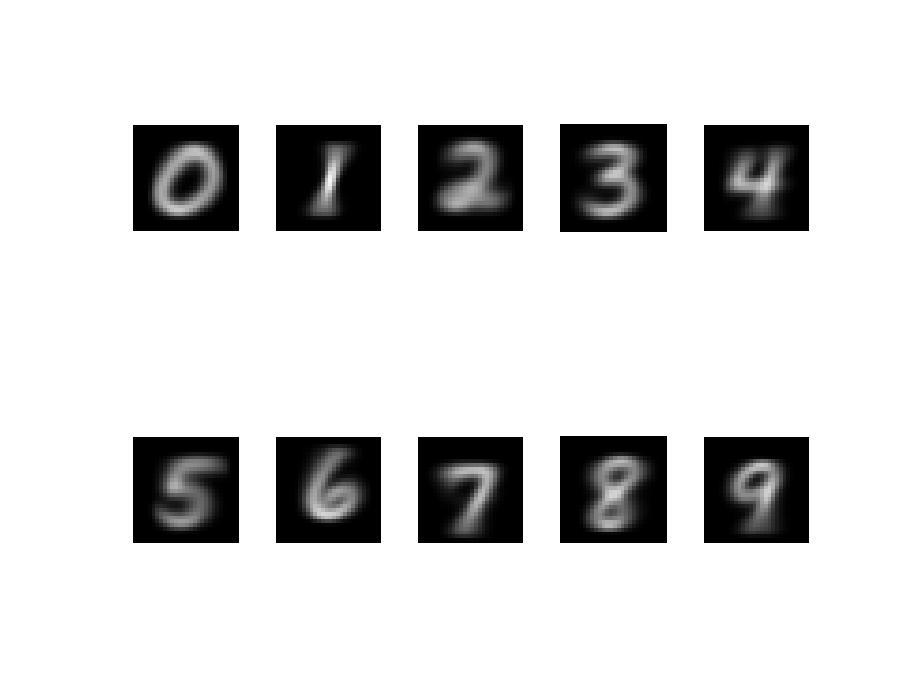
\includegraphics[width=0.9\columnwidth]{mnist_average_training_image.eps}
%     \end{center}
%     \caption{The 10 images are the averages of all of the training images for each digit.
%         They represent what a {\it typical} digit should look like for each of the 10
%     digits.}
%     \label{fig:mnist_average}
% \end{figure}
% 
% 


\begin{problem}
    Find the largest eigenvalue of the matrix $A$ WITHOUT using the built in
    ``\mcode{eig}'' or ``\mcode{eigs}'' commands in MATLAB.
    \[ A = \begin{pmatrix} 1 & 2 & 3 & 4 \\ 5 & 6 & 7 & 8 \\ 9 & 0 & 1 & 2 \\ 3 & 4 & 5 &
        6 \end{pmatrix} \]
\end{problem}
\hint{
    You should be using the power method.
}


\begin{problem}
    Find a least square cubic function that best fits the following data. Solve this
    problem with Excel and with MATLAB using the normal equations.
    \begin{center}
        \begin{tabular}{|c|c|}
            \hline
            $x$ & $y$ \\\hline \hline
            0   & 1.0220\\
            0.0500&   1.0174\\
            0.1000&   1.0428\\
            0.1500&   1.0690\\
            0.2000&   1.0505\\
            0.2500&   1.0631\\
            0.3000&   1.0458\\
            0.3500&   1.0513\\
            0.4000&   1.0199\\
            0.4500&   1.0180\\
            0.5000&   1.0156\\
            0.5500&   0.9817\\
            0.6000&   0.9652\\
            0.6500&   0.9429\\
            0.7000&   0.9393\\
            0.7500&   0.9266\\
            0.8000&   0.8959\\
            0.8500&   0.9014\\
            0.9000&   0.8990\\
            0.9500&   0.9038\\
            1.0000&   0.8989 \\\hline
        \end{tabular}
    \end{center}
\end{problem}



\begin{thm}[Eigen-Structure of Symmetric Matrices]\label{thm:symmetric_matrix_thm}
    If $A$ is a symmetric matrix with eigenvalues $\lambda_1, \lambda_2, \ldots,
    \lambda_n$ then $|\lambda_1| > |\lambda_2| > \cdots > |\lambda_n|$.  Furthermore, the
    eigenvectors will be orthogonal to each other. 
\end{thm}


\begin{problem}
    For symmetric matrices we can build an extension to the Power Method in order
    to find the second most dominant eigen-pair for a matrix $A$.  Theorem
    \ref{thm:symmetric_matrix_thm} suggests the following method for finding the second
    dominant eigen-pair for a symmetric matrix.  This method is called the {\bf deflation
    method}.
    \begin{itemize}
        \item Use the power method to find the dominant eigenvalue and eigenvector.
        \item Start with a random unit vector of the correct shape.
        \item Multiplying your vector by $A$ will {\it pull it toward} the dominant
            eigenvector.  After you multiply, project your vector onto the dominant
            eigenvector and find the projection error.  
        \item Use the projection error as the new approximation for the eigenvector.
    \end{itemize}    

    Note that the deflation method is really exactly the same as the power method with the
    exception that we orthogonalize at every step.  Hence, when you write your code expect
    to only change a few lines from your Power method.

    Write a
    MATLAB function \mcode{MyPower2} to find the second largest eigenvalue and
    eigenvector pair by putting the deflation method into practice. Test your code on a
    \underline{symmetric} matrix $A$ and compare against MATLAB's \mcode{eig} command.
    Your code needs to work on symmetric matrices of arbitrary size and you need to write
    test code that clearly shows the error between your calculated eigenvalue and MATLAB's
    eigenvalue as well as your calculated eigenvector and MATLAB's eigenvector.\\ To
    guarantee that you start with a symmetric matrix you can use the following code.
\begin{lstlisting}
N = 40; % size of the matrix ... make this large-ish
A = rand(N,N);
A = A'*A; % this will be a random symmetric NxN matrix.
\end{lstlisting}
\end{problem}
\hint{
    Technically speaking you don't have to orthogonalize at every step so if you want to
    make your code more efficient you can orthogonalize every $k^{th}$ step (for your
    choice of $k$).  It would be cool to check what this does to the efficiency of your
    algorithm.
}





\newpage\section{Projects}
In this section we propose several ideas for projects related to numerical linear algebra.
These projects are meant to be open ended, to encourage creative mathematics, to push your
coding skills, and to require you to write and communicate your mathematics.  Take the
time to read Appendix \ref{app:writing_projects} before you write your final solution.

\subsection{Applications of the Singular Value Decomposition}
The singular value decomposition (SVD) is a matrix factorization that can be thought of as
the generalization of the eigenvalue problem for non-square matrices.  We wish to take a
matrix $A$ that has size $m \times n$ and factor it into three matrices, $U$, $\Sigma$,
and $V$ such that 
\[ A = U \Sigma V^T \]
where $U$ is an $m \times m$ orthonormal matrix, $\Sigma$ is an $m \times n$ rectangular
diagonal matrix, and $V$ is and $n \times n$ orthonormal matrix.  Recall that an
orthonormal matrix
is a matrix where the transpose is the inverse.  That is, $UU^T = I_{m \times m}$ and $VV^T
= I_{n \times n}$. The columns of $U$ are called the left singular vectors of $A$ and are
the eigenvectors of the matrix $AA^T$.  The columns of $V$ are called the right singular
vectors of $A$ and are the eigenvectors of the matrix $A^TA$.  The diagonal entries of
$\Sigma$ are the square roots of the non-zero eigenvalues of both $AA^T$ and $A^TA$.

It is probably best to have a look at an example (modified from
\footnote{\href{http://www.d.umn.edu/~mhampton/m4326svd_example.pdf}{http://www.d.umn.edu/~mhampton/m4326svd\_example.pdf}}).  Consider the matrix 
\[ A = \begin{pmatrix} 3 & 2 & 1 \\ 2 & 3 & -2 \end{pmatrix}. \]
We would like to factor $A$ into $A = U \Sigma V^T$.  First we find the eigenvalues and
eigenvectors of $AA^T$.  It is left to the reader to verify\footnote{That means that you
should stop what you're doing and actually verify this result!} that the eigenvalues are
$\lambda_1 = 25$ and $\lambda_2 = 9$.  Hence, the singular values are $\sigma_1 = 5$ and
$\sigma_2 = 3$.  Next we find the right singular vectors (the columns of $V$) by finding
an orthonormal set of eigenvectors of $A^TA$.  This too is left to the reader to verify
that the matrix $V$ is 
\[ V = \begin{pmatrix}
        1/\sqrt{2} & 1/\sqrt{18} & 2/3 \\
        1/\sqrt{2} & -1/\sqrt{18} & -2/3 \\
        0 & 4/\sqrt{18} & -1/3 
    \end{pmatrix}. \]
The reader should also observe that the columns of $V$ are all orthogonal to each other as
well as being unit vectors.

We now know that 
\[ A = U \Sigma V^T = U \begin{pmatrix} 5 & 0 & 0 \\ 0 & 3 & 0 \end{pmatrix} \begin{pmatrix} 1/\sqrt{2} & 1/\sqrt{2} & 0 \\ 1/\sqrt{18} & -1/\sqrt{18} &
        4/\sqrt{18} \\ 2/3 & -2/3 & -1/3 \end{pmatrix} \]
Since $V$ is an orthogonal matrix and the singular values $\sigma_1$ and $\sigma_2$ are
non-zero we can see that 
\[ U = AV\Sigma^\dagger \]
where 
\[ \Sigma^\dagger = \begin{pmatrix} 1/5 & 0 \\ 0 & 1/3 \\ 0 & 0 \end{pmatrix}. \]
After a bit of computation we finally find that 
\[ U = \begin{pmatrix} 1/\sqrt{2} & 1/\sqrt{2} \\ 1/\sqrt{2} & -1/\sqrt{2} \end{pmatrix}
        \]
and hence
\[ A = \begin{pmatrix} 1/\sqrt{2} & 1/\sqrt{2} \\ 1/\sqrt{2} & -1/\sqrt{2} \end{pmatrix} \begin{pmatrix} 5 & 0 & 0 \\ 0 & 3 & 0 \end{pmatrix} \begin{pmatrix} 1/\sqrt{2} & 1/\sqrt{2} & 0 \\ 1/\sqrt{18} & -1/\sqrt{18} &
        4/\sqrt{18} \\ 2/3 & -2/3 & -1/3 \end{pmatrix} \]
We leave it to the reader to check that this is correct.  

Obviously this is not a computation that you typically do by hand.  You should have SVD
code handy that does this entire algorithm.  MATLAB also has a built-in svd code that is
optimized to run faster than the one that we built in class.  You are welcome to use the
built-in svd MATLAB routine in this project.

\subsection*{Problem Statement}
There are many applications of the singular value decomposition.  In fact, the SVD is
considered one of the most useful and widely used matrix decompositions in the linear
algebra arsenal.  Your job for this project will be to explore two of those applications.
Below you will find a brief list of some of the primary uses for the singular value
decomposition.  Some of them are rather intricate and some are fairly straight forward to
implement, but I leave it to you to choose applications that are of interest to you.

\subsection*{Your Tasks}
You and your partner will choose two applications and do the following:
\begin{enumerate}
    \item[(a)] implement non-trivial examples of the application 
    \item[(b)] write a brief technical report detailing how each application works
        (including all of the mathematical details), and
    \item[(c)] write a 1 paragraph non-technical summary describing
        each application and how it works.  The audience for this non-technical summary is
        any reasonably educated, but not necessarily mathematically sophisticated,
        adult.
\end{enumerate}

Note: All code for this project must be uniquely yours or your partners.  

\subsection*{List of Applications}
Each of the following applications of the singular value decomposition is followed by a
brief description (paraphrased from various web sources linked in the footnotes).  Use
this to guide your choice.
\begin{description}
    \item[Principal Component Analysis:] (PCA) is a statistical tool that allows you to
        convert a set of possibly correlated data observations into uncorrelated
        components.  This is a method of data reduction that, in some sense, reduces how much
        data is actually influential in your data set.  PCA takes
        a potentially large data set and reduces it down to its {\it principal
        components} that are the most influential on the data.  PCA itself has many
        applications ranging from statistics to signal processing.  If you choose this
        application you will need to implement PCA on a non-trivial data set of your
        choosing.  There are several sample data sets on the web but the
        ones that are used for explanation are often quite trivial in size
        and scope.  \footnote{\href{https://en.wikipedia.org/wiki/Principal_component_analysis}{PCA
        Wiki page: en.wikipedia.org/wiki/Principal\_component\_analysis}}  Absolutely do
        not just make up your own data set.
    \item[Low Rank Image Approximations:] There are literally hundreds of ways to trim
        information from images while retaining the most important parts of the image.  One of the simplest is to apply the singular value decomposition to the
        rectangular image (either in grayscale or separately for each RBG matrix).  Then
        you can zero out the lower value singular values and vectors and then rebuild the
        image.  The
        low rank approximation (really just another type of data reduction) does obviously lead to some loss of information but up to a certain point
        this loss of information is un-noticeable to the human eye.  If you choose this
        application you need to supply your own images as well as give several examples of
        how low rank approximation changes the image.  You should also 
        explore how low rank approximations can be used as a method of image compression.  and give some sort of mathematical measure
        defining how much data reduction was performed along with the re-generated images
        so we can see the
        reduction.\footnote{\href{http://math.arizona.edu/~brio/VIGRE/ThursdayTalk.pdf}{A
        Sample of the Image Compression Technique: math.arizona.edu/\~brio/VIGRE/ThursdayTalk.pdf}}
    \item[Recommender Systems:] You run in the {\it recommender systems} all the time.
        Amazon seems to know what other books you might like, NetFlix seems to know what
        other movies you might like, and the list goes on.  One way to perform the
        matching behind the scenes in a
        recommender system is to use the SVD along with data reduction techniques (just
        like with PCA and image compression).  If you choose this application you need to
        provide a non-trivial example of a recommender system preferably of real data
        released from one of the large common sites (NetFlix, Amazon,
        etc.).\footnote{\href{http://www.cs.carleton.edu/cs_comps/0607/recommend/recommender/svd.html}{The
            idea of SVD for Recommender Systems:
        http://www.cs.carleton.edu/cs\_comps/0607/recommend/recommender/svd.html}}
        \footnote{\href{http://robotics.stanford.edu/~ronnyk/WEBKDD2000/papers/sarwar.pdf}{Paper
            about Recommender Systems:
        http://robotics.stanford.edu/~ronnyk/WEBKDD2000/papers/sarwar.pdf}}
    \item[The Kabsh Algorithm:] This is an algorithm for calculating the optimal rotation
        matrix that minimizes the error between two sets of points.  This
        is a useful method in comparing molecular structures (including proteins) but is
        not just used in mathematical biology.  If you
        choose this application then you need to provide several non-trivial examples of
        how the method works and what it is that you are finding.
        \footnote{\href{https://en.wikipedia.org/wiki/Kabsch_algorithm}{Wiki page for
        Kabsh Algorithm: https://en.wikipedia.org/wiki/Kabsch\_algorithm} }
%     \item[Image Deblurring:] A method for taking a blurred image and returning it to the
%         sharp (or nearly sharp) original image is related to the singular value
%         decomposition.  This method requires you to know the way in which the image was
%         blurred but the inverse of the process is usually contaminated with noise so
%         taking a simple linear inverse neither works nor makes sense.  Follow the link in
%         the footnote for a full textbook on the image deblurring problem.
%         \footnote{\href{http://web.ipac.caltech.edu/staff/fmasci/home/astro_refs/ImageDeblurring_2006.pdf}{Image
%         Deblurring Text: http://web.ipac.caltech.edu/staff/fmasci/home/astro\_refs/ImageDeblurring\_2006.pdf}} 
    \item[Choose Your Own Adventure:] If you happen upon an interesting and non-trivial
        application of the singular value decomposition then you are welcome to use this
        as one of your two applications.  Just be sure that you can implement it 
        and that you can fully explain what you're doing. A decent place to start is the
        applications section of the SVD Wiki page.
        \footnote{\href{https://en.wikipedia.org/wiki/Singular_value_decomposition}{SVD
            Wiki:
        https://en.wikipedia.org/wiki/Singular\_value\_decomposition}}
\end{description}


\newpage\subsection{The Google Page Rank Algorithm}


In this project you will discover how the PageRank algorithm works to give the most relevant
information as the top hit on a Google search.  

Search engines compile large indexes of the dynamic information on the Internet so they
are easily searched.  This means that when you do a Google search, you are not actually
searching the Internet; instead, you are searching the indexes at Google.

When you type a query into Google the following two steps take place:
\begin{enumerate}
    \item Query Module: The query module at Google converts your natural language into a
        language that the search system can understand and consults the various indexes
        at Google in order to answer the query.  This is done to find the list of relevant
        pages.
    \item Ranking Module: The ranking module takes the set of relevant pages and ranks
        them. The outcome of the ranking is an ordered list of web pages such
        that the pages near the top of the list are most likely to be what you desire from
        your search. This ranking is the same as assigning a {\it popularity score} to
        each web site and then listing the relevant sites by this score.  
\end{enumerate}

This section focuses on the Linear Algebra behind the Ranking Module developed by the
founders of Google: Sergey Brin and Larry Page.  Their algorithm is called the
\emph{PageRank algorithm}, and you use it every single time you use Google's search
engine.


In simple terms: {\it A webpage is important if it is pointed to by other important
pages}.

The Internet can be viewed as a directed graph (look up this term
\href{https://en.wikipedia.org/wiki/Directed_graph}{here on Wikipedia}) where the nodes
are the web pages and the edges are the hyperlinks between the pages. The hyperlinks into a
page are called {\it inlinks}, and the ones pointing out of a page are called {\it
outlinks}.  In essence, a hyperlink from my page to yours is my endorsement of your page.
Thus, a page with more recommendations must be more important than a page with a few
links.  However, the status of the recommendation is also important. 

Let us now translate this into mathematics. To help understand
this we first consider the small web of six pages shown in Figure
\ref{fig:example_graph} (a graph of the router level of the internet can be found
\href{https://personalpages.manchester.ac.uk/staff/m.dodge/cybergeography/atlas/lumeta_large.jpg}{here}).  The links between the
pages are shown by arrows. An arrow pointing into a node is an {\it inlink}
and an arrow pointing out of a node is an {\it outlink}. In Figure
\ref{fig:example_graph}, node 3 has three outlinks (to nodes 1, 2, and 5)
and 1 inlink (from node 1).

\begin{figure}[ht]
    \begin{center}
        \begin{tikzpicture}
            \draw (0,0) node[circle,draw]{3};
            \draw (-1,1) node[circle,draw]{1};
            \draw (1,1) node[circle,draw]{2};
            \draw (-1,-1) node[circle,draw]{6};
            \draw (1,-1) node[circle,draw]{5};
            \draw (0,-2) node[circle,draw]{4};
        %
            \draw[<->] (-0.25,0.25) -- (-0.75,0.75);
            \draw[->] (-0.65,1) -- (0.65,1);
            \draw[->] (0.25,0.25) -- (0.75,0.75);
            \draw[->] (0.25,-0.25) -- (0.75,-0.75);
            \draw[->] (0.65,-1) -- (-0.65,-1);
            \draw[<->] (-0.75,-1.25) -- (-.25,-1.75);
            \draw[<->] (0.75,-1.25) -- (0.25,-1.75);
        \end{tikzpicture}
    \end{center}
        \caption{Sample graph of a web with six pages.}
        \label{fig:example_graph}
\end{figure}

We will first define some notation in the PageRank algorithm:
\begin{itemize}
    \item $|P_i|$ is the number of outlinks from page $P_i$
    \item $H$ is the {\it hyperlink} matrix defined as 
        \[ H_{ij} = \left\{ \begin{array}{cl} \frac{1}{|P_j|}, & \text{if there is a link
            from node $j$ to node $i$} \\ 0, & \text{otherwise} \end{array} \right. \]
        where the ``$i$'' and ``$j$'' are the row and column indices respectively.  
    \item $\bx$ is a vector that contains all of the PageRanks for the individual pages.
\end{itemize}

The PageRank algorithm works as follows:
\begin{enumerate}
    \item Initialize the page ranks to all be equal. This means that our initial
        assumption is that all pages are of equal rank.  In the case of Figure
        \ref{fig:example_graph} we would take $\bx_0$ to be 
        \[ \bx_0 = \begin{pmatrix} 1/6 \\ 1/6 \\ 1/6 \\ 1/6 \\ 1/6 \\ 1/6 \end{pmatrix}. \]
    \item Build the hyperlink matrix.  \\ As an example we'll consider node 3 in Figure
        \ref{fig:example_graph}.  There are three outlinks from node 3 (to nodes 1, 2, and
        5).  Hence $H_{13}=1/3$, $H_{23} = 1/3$, and $H_{53} = 1/3$ and the partially
        complete hyperlink matrix is
        \[ H = \begin{pmatrix} 
                - & - & 1/3 & - & - & - \\
                - & - & 1/3 & - & - & - \\
                - & - & 0   & - & - & - \\
                - & - & 0   & - & - & - \\
                - & - & 1/3 & - & - & - \\
                - & - & 0   & - & - & - 
            \end{pmatrix} \]
    \item The difference equation $\bx_{n+1} = H \bx_n$ is used to iteratively refine the
        estimates of the page ranks.  You can view the iterations as a person visiting a
        page and then following a link at random, then following a random link on the next
        page, and the next, and the next, etc.  Hence we see
        that the iterations evolve exactly as expected for a difference equation.
        \begin{center}
            \begin{tabular}{|c|c|}
                \hline
                Iteration & New Page Rank Estimation \\ \hline \hline
                0 & $\bx_0$ \\
                1 & $\bx_1 = H \bx_0$ \\
                2 & $\bx_2 = H \bx_1 = H^2 \bx_0$ \\
                3 & $\bx_3 = H \bx_2 = H^3 \bx_0$ \\
                4 & $\bx_4 = H \bx_3 = H^4 \bx_0$ \\
                \vdots & \qquad \vdots \\
                $k$ & $\bx_k = H^k \bx_0$ \\ \hline
            \end{tabular}
        \end{center}
    \item When a steady state is reached we sort the resulting vector $\bx_k$ to give the
        page rank. The node (web page) with the highest rank will be the top search
        result, the second highest rank will be the second search result, and so on.
\end{enumerate}

It doesn't take much to see that this process can be very time consuming.  Think about
your typical web search with hundreds of thousands of hits; that makes a square matrix $H$
that has a size of hundreds of thousands of entries by hundreds of thousands of entries!
The matrix multiplications alone would take many minutes (or possibly many hours) for
every search! \dots but Brin and Page were pretty smart dudes!!


We now state a few theorems and definitions that will help us simplify the iterative
PageRank process.
\begin{thm}\label{thm:eigen_expand}
    If $A$ is an $n \times n$ matrix with $n$ linearly independent eigenvectors $\bv_1,
    \bv_2, \bv_3,$ $\ldots, \bv_n$ and associated eigenvalues $\lambda_1, \lambda_2,
    \lambda_3, \ldots, \lambda_n$ then for any initial vector $\bx \in \mathbb{R}^n$ we
    can write $A^k \bx$ as
    \[ A^k \bx = c_1 \lambda_1^k \bv_1 + c_2 \lambda_2^k \bv_2 + c_3 \lambda_3^k \bv_3 +
        \cdots c_n \lambda_n^k \bv_n \]
    where $c_1, c_2, c_3, \ldots, c_n$ are the constants found by expressing $\bx$ as a
    linear combination of the eigenvectors. \\Note: We can assume that the eigenvalues are ordered
    such that $\lambda_1 \ge \lambda_2 \ge \lambda_3 \ge \cdots \ge \lambda_n$.
\end{thm}
\begin{proof}
    (Prove the preceding theorem)
\end{proof}

\begin{definition}
    A {\bf probability vector} is a vector with entries on the interval $[0,1]$ that add up to 1. 
\end{definition}
\begin{definition}
    A {\bf stochastic matrix} is a square matrix whose columns are probability vectors.
\end{definition}

\begin{thm} \label{thm:largest_ev_stochastic}
    If $A$ is a stochastic $n \times n$ matrix then $A$ will have $n$ linearly independent
    eigenvectors.  Furthermore, the largest eigenvalue of a stochastic matrix will
    \underline{always} be $\lambda_1 = 1$ and the smallest eigenvalue  will always be
    nonnegative: $0 \le \lambda_n < 1$.
\end{thm}

Some of the following tasks will ask you to {\it prove} a statement or a theorem.  This
means to clearly write all of the logical and mathematical reasons why the statement is
true. Your proof should be absolutely crystal clear to anyone with a similar mathematical
background \dots if you are in doubt then have a peer from a different group read your
proof to you \underline{out loud}.

\begin{problem}
    Finish writing the hyperlink matrix $H$ from Figure \ref{fig:example_graph}.
\end{problem}

\begin{problem}
    Write MATLAB code to implement the iterative process defined previously. Make a plot
    that shows how the rank evolves over the iterations.
\end{problem}


\begin{problem}
    What must be true about a collection of $n$ pages such that an $n\times n$
        hyperlink matrix $H$ is a stochastic matrix.
\end{problem}

The statement of the next theorem is incomplete, but the proof is given to you.  Fill in
the blank in the statement of the theorem and provide a few sentences supporting your
answer.
\begin{thm}\label{thm:steady}
    If $A$ is an $n \times n$ stochastic matrix and $\bx_0$ is some initial vector
    for the difference equation $\bx_{n+1} = A \bx_n$, then the steady state
    vector is
    \[ \bx_{equilib} = \lim_{k \to\infty} A^k \bx_0 = \underline{\hspace{1in}}. \]
\end{thm}
\begin{proof}
    First note that $A$ is an $n \times n$ stochastic matrix so from Theorem
    \ref{thm:largest_ev_stochastic} we know that there are $n$ linearly
    independent eigenvectors.  We can then substitute
    the eigenvalues from Theorem \ref{thm:largest_ev_stochastic} in Theorem
    \ref{thm:eigen_expand}. Noting that if $0<\lambda_j<1$ we have $\lim_{k \to
    \infty} \lambda_j^k = 0$ the result follows immediately.
\end{proof}
\begin{problem}
    Discuss how Theorem \ref{thm:steady} greatly simplifies the PageRank iterative process
    described previously.  In other words: there is no reason to iterate at all.  Instead,
    just find \underline{\hspace{1in}}.
\end{problem}
\begin{problem}
\item Now use the previous two problems to find the resulting PageRank vector from the web in Figure
    \ref{fig:example_graph}?  Be sure to rank the pages in order of importance.
    Compare your answer to the one that you got in problem 2.
\end{problem}


\begin{problem}
    Consider the web in Figure \ref{fig:graph2}.
        \begin{enumerate}
            \item[(a)] Write the $H$ matrix and find the initial state $\bx_0$, 
            \item[(b)] Find
                steady state PageRank vector using the two different methods described:
                one using the iterative difference equation and the other using Theorem
                \ref{thm:steady} and the dominant eigenvector.
            \item[(c)] Rank the pages in order of importance.
        \end{enumerate}
\end{problem}
\begin{figure}[ht!]
    \begin{center}
        \begin{tikzpicture}
            \draw (0,0) node[circle,draw]{3};
            \draw (-1,1) node[circle,draw]{1};
            \draw (1,1) node[circle,draw]{2};
            \draw (-1,-1) node[circle,draw]{6};
            \draw (1,-1) node[circle,draw]{5};
            \draw (0,-2) node[circle,draw]{4};
            \draw (-2,0) node[circle,draw]{7};
            \draw (-2,-2) node[circle,draw]{8};
        %
            \draw[<-] (-0.25,0.25) -- (-0.75,0.75);
            \draw[->] (-0.65,1) -- (0.65,1);
            \draw[<->] (0.25,0.25) -- (0.75,0.75);
            \draw[<->] (0.25,-0.25) -- (0.75,-0.75);
            \draw[->] (0.65,-1) -- (-0.65,-1);
            \draw[<->] (-0.75,-1.25) -- (-.25,-1.75);
            \draw[<->] (0.75,-1.25) -- (0.25,-1.75);
            \draw[<->] (-1.75,0.25) -- (-1.25,0.75);
            \draw[<->] (-1.65,0) -- (-0.35,0);
            \draw[<-] (-1.75,-0.25) -- (0.7,-0.8);
            \draw[->] (-2,-0.35) -- (-2,-1.65);
            \draw[<->] (-1.65,-2) -- (-0.35,-2);
        \end{tikzpicture}
    \end{center}
    \caption{Graph of a web with eight pages.}
    \label{fig:graph2}
\end{figure}


\begin{problem}
    One thing that we didn't consider in this version of the Google Page Rank algorithm is
    the random behavior of humans.  One, admittedly slightly naive, modification that we
    can make to the present algorithm is to assume that the person surfing the web will
    randomly jump to any other page in the web at any time.  For example, if someone is on
    page 1 in Figure \ref{fig:graph2} then they could randomly jump to any page 2 - 8.
    They also have links to pages 2, 3, and 7.  That is a total of 10 possible next steps
    for the web surfer.  There is a $2/10$ chance of heading to page 2.  One of those is
    following the link from page 1 to page 2 and the other is a random jump to page 2
    without following the link.  Similarly, there is a $2/10$ chance of
    heading to page 3, $2/10$ chance of heading to page 7, and a $1/10$ chance of randomly
    heading to any other page.

    Implement this new algorithm, called the {\it random surfer algorithm}, on the web in
    Figure \ref{fig:graph2}.  Compare your ranking to the non-random surfer results from
    the previous problem.
\end{problem}



% \newpage\subsection{Principal Component Analysis (Incomplete)}

\chapter{Numerical Ordinary Differential Equations}\label{ch:odes}

In this chapter we will solve first order ordinary differential equations of the form
\[ y'(t) = f(t,y(t)) \]
with initial condition $y(t_0)=y_0$ for $t\ge t_0$.  These are known as ``ordinary''
differenatial equations since they contain only ``ordinary'' derivatives; not partial
derivatives.  Given that we are solving the problem with given intial information these
are also called intial value problems.  

\section{Euler, Runge-Kutta, and Friends}
The notion of approximating solutions to differential equations is simple: make a discrete
approximation to the derivative and step forward through time as a difference equation.
The fun part is making the approximation to the derivative(s).  There are many methods for
approximating derivatives, and that is exactly where we'll start.

\begin{technique}[Euler's Method]
    You're probably already familiar with Euler's method for approximating the solution to
    a differential equation. We want to approximate a solution to $y'(t) = f(t,y(t))$.
    Recall from Problem \ref{prob:num_diff_first_order} that 
    \[ y'(t) = \frac{y(t+h) - y(t)}{h} + \mathcal{O}(h) \]
    so the differential equation $y'(t) = f(t,y(t))$ becomes
    \[ \frac{y(t+h) - y(t)}{h} \approx f(t,y(t)). \]
    Rewriting as a difference equation, letting $y_{n+1} = y(t_n+h)$ and $y_n = y(t_n)$,
    we get
    \begin{flalign}
        y_{n+1} = y_n + h f(t_n , y_n)
        \label{eqn:Eulers_method}
    \end{flalign}
%     \begin{enumerate}
%         \item Recall that a taylor series for a continuously differentiable function
%             $f(x)$ centered at $x=a$ is
%             \[ f(x) = f(c) + \frac{f'(a)}{1!}(x-a) + \frac{f''(a)}{2!}(x-a)^2 +
%                 \frac{f^{(3)}(a)}{3!}(x-a)^3 + \frac{f^{(4)}(a)}{4!}(x-a)^4 + \cdots \]
%         \item Write a Taylor series for $y(t)$ by replacing $f$ with $y$, $x$ with $t+h$
%             and $a$ with $t$
%             \[ y(t+h) = \dots\]
% %             \teacher{
% %                 \[ y(t+h) = y(t) + y'(t)h + \frac{y''(t)}{2!} h^2 + \cdots \]
% %             }
%         \item Since we know that $y'(t) = f(t,y(t))$ we can rewrite the Taylor series as
%             \[ y(t+h) = \dots \]
% %             \teacher{
% %                 \[ y(t+h) = y(t) + hf(t,y(t)) + \frac{y''(t)}{2!} h^2 + \cdots \]
% %             }
%         \item Now we can look at this as a difference equation that is ready made for
%             numerical implementation with a loop:
%             \[ y_{n+1} = y_n + h f(t_n,y_n) + \mathcal{O}(h^2)\]
%         \item The {\it approximation error} for Euler's method is actually not second
%             order as the previous equation would suggest.  Instead, if we rearrange to
%             write Euler's formula as an approximation of the derivative we get
%             \[ \frac{y_{n+1}-y_n}{h} = f(t_n,y_n) + \mathcal{O}(h). \]
%             What does this formula tell you about the accuracy of Euler's method?
%     \end{enumerate}
\end{technique}

A way to think about Euler's method is that at a given point, the slope is approximated by
the value of the right-hand side of the differential equation and then we step forward $h$
units in time following that slope.  Figure \ref{fig:Euler} shows a depiction of the idea.
Notice in the figure that in regions of high curvature Euler's method will overshoot the
exact solution to the differential equation.  However, taking $h \to 0$ theoretically
gives the exact solution at the tradeoff of needing infinite computational resources.

\begin{figure}[ht!]
    \begin{center}
        \begin{tikzpicture}
            \begin{axis}[axis lines=center, grid, xmin=0, xmax=5, ymin=0, ymax=5,
                domain=0:5, xlabel={$t$}, ylabel={$y$}, legend pos=outer north east]
                \addplot[very thick, smooth, black] {0.25*(x-2)^2+2};
                \addlegendentry{Exact solution};
                \addplot[red, dashed, very thick]
                coordinates{(0,3)(1,2)(2,1.5)(3,1.5)(4,2)(5,3)};
                \addlegendentry{Euler with $h=1$};
                \addplot[blue, dotted, very thick]
                coordinates{(0,3)(0.5,2.5)(1,2.125)(1.5,1.875)(2,1.75)(2.5,1.75)(3,1.875)(3.5,2.125)(4,2.5)(4.5,3)(5,3.625)};
                \addlegendentry{Euler with $h=0.5$};
            \end{axis}
        \end{tikzpicture}
    \end{center}
    \caption{A depiction of Euler's method with step size $h=1$ (red) and $h=0.5$ (blue).}
    \label{fig:Euler}
\end{figure}


\begin{problem}
    Write code to implement Euler's method for initial value problems.  Your MATLAB
    function should accept as input: $f(t,y)$, \texttt{tmin}, \texttt{tmax}, the number of
    grid points (the value of $h = \Delta t$ should be calculated within your code), and
    an intial condition.  The output should be vectors for $t$ and $y$.\\
    \verb|function [t,y] = MyEuler1D(f,tmin,tmax,num_pts,IC)| \\
    Test your code on a first order differential equation where you know the answer and
    then test your code on the differential equation
    \[ y' = -\frac{1}{3}y+\sin(t) \quad \text{where} \quad y(0) = 1. \]
\end{problem}

\begin{problem}\label{prob:2dPredPrey}
    Write code that implements a 2D version of Euler's method that will solve a system of
    two differential equations in two dependent variables.  Test your code on the
    following problem by showing a time evolution plot (time on $x$ and populations on
    $y$) as well as a phase plot ($x$ on the $x$ and $y$ on the $y$ with time understood
    implicitly):\\
    {\bf The Lotka-Volterra Predator-Prey Model:}\\
    Let $x(t)$ denote the number of rabbits (prey) and $y(t)$ denote the number of foxes
    (prey) at time $t$.  The relationship between the species can be modeled by the
    classic 1920's Lotka-Volterra Model:
    \[ \left\{ \begin{array}{ll} x' &= \alpha x - \beta xy \\ y' &= -\delta y + \gamma xy
        \end{array} \right. \]
    where $\alpha, \beta, \gamma,$ and $\delta$ are positive constants.  For this
    problems take $\alpha \approx 1$, $\beta \approx 0.05$, $\gamma \approx 0.01$, and
    $\delta \approx 1$.  Be sure to explain the meaning of each of the parameters and each
    of the components of the model.
\end{problem}

\begin{technique}[The Midpoint Method]
    Now we begin the journey of creating better solvers than Euler's method.  The midpoint method
    is defined by first taking a half step with Euler's method to approximate a solution
    at time $t_{n+1/2} \equiv (t_n + t_{n+1})/2$ and then taking a full step using the
    value of $f$ at $t_{n+1/2}$ and the approximate $y_{n+1/2}$.
    \begin{flalign*}
        y_{n+1/2} &= y_n + \frac{h}{2} f(t_n, y_n) \\
        y_{n+1} &= y_n + h f(t_{n+1/2}, y_{n+1/2})
    \end{flalign*}
    Note: Indexing by $1/2$ in a computer is nonsense.  Instead, we implement the midpoint
    method with:
    \begin{flalign*}
        y_{temp} &= y_n + \frac{h}{2} f(t_n, y_n) \\
        y_{n+1} &= y_n + h f\left( \frac{t_n+t_{n+1}}{2}, y_{temp}\right)
    \end{flalign*}

\end{technique}

\begin{problem}
    Write MATLAB code to implement the midpoint method\\
    \verb|function [t,y]=MyMidpointMethod(f,tmin,tmax,num_pts,IC)| \\
\end{problem}

\begin{problem}
    Test your midpoint method code against your Euler1D code on the same single variable
    ODE as before.  You will likely see very little difference on a very small step size
    (equivalently, a large number of points), but for a smaller number of points there
    will be a remarkable difference.  
\end{problem}


\begin{problem}
    {\bf The Runge-Kutta Method:}\\
    Another method for approximating the solution to a first order initial value problem
    is to take several approximations and average them in a smart way.  The Runge-Kutta 4
    method is one (of many) such methods.  In this method, each $k_j$ is an approximation
    of the slope and we combine them in as a weighted average in the end.
    \begin{flalign*}
        k_1 &= f(t_n, y_n) \\
        k_2 &= f(t_n + \frac{h}{2} , y_n + \frac{h}{2} k_1) \\
        k_3 &= f(t_n + \frac{h}{2} , y_n + \frac{h}{2} k_2) \\
        k_4 &= f(t_n + h , y_n + h k_3) \\
        y_{n+1} &= y_n + \frac{h}{6} \left( k_1 + 2 k_2 + 2 k_3 + k_4 \right)
    \end{flalign*}

    Write a MATLAB function that implements the Runge-Kutta 4 method in one dimension.\\
    \texttt{function [t,y]=MyRk4(f,tmin,tmax,num\_pts,IC)} \\
    Test the problem on a known differential equation.
\end{problem}


\begin{problem}
    Modify your Runge-Kutta 4 code to work for two dependent variables.  I'll get you
    started:\\We want to solve
    \[ \left\{ \begin{array}{ll} x' &= f(t,x,y) \\ y' &= g(t,x,y) \end{array} \right. \]
    and to do so we extend the Runge Kutta method as
    \begin{flalign*}
        k_1 &= f(t_n,x_n, y_n) \\
        q_1 &= g(t_n,x_n, y_n) \\
        k_2 &= f(t_n + \frac{h}{2} ,x_n+\frac{h}{2} k_1, y_n + \frac{h}{2} q_1) \\
        q_2 &= g(t_n + \frac{h}{2} ,x_n+\frac{h}{2} k_1, y_n + \frac{h}{2} q_1) \\
        k_3 &= \dots \\
        q_3 &= \dots \\
        k_4 &= \dots \\
        q_4 &= \dots \\
        x_{n+1} &= x_n + \frac{h}{6} \left( k_1 + 2 k_2 + 2 k_3 + k_4 \right)\\
        y_{n+1} &= y_n + \frac{h}{6} \left( q_1 + 2 q_2 + 2 q_3 + q_4 \right)
    \end{flalign*}
    
    Test your code on
    the predator prey model in problem \ref{prob:2dPredPrey}.
\end{problem}


\begin{problem}
    Solving systems of ordinary differential equations would become challenging if we were
    to continue coding in the same way as in the previous problem. Write a MATLAB function
    that accepts any number of right-hand sides from a system of differential equations
    and then leverages the fact that MATLAB works very well with vectors to create Euler
    and Runge-Kutta solutions to these systems. Devise several systems to test your code
    (including 1D and 2D).
\end{problem}


\section{Implicit Methods and Shooting Methods}
\begin{problem}
    The major trouble with the RK (and midpoint) methods is that they take many more
    function evaluations than Euler's method.  We can improve upon Euler's method in the
    following way:\\
    We want to solve $y' = f(t,y)$ so:
    \begin{enumerate}
        \item Approximate the derivative by looking forward in time(!)
            \[ \frac{y_{n+1} - y_n}{h} \approx f(t_{n+1} , y_{n+1}) \]
        \item Rearrange to get the difference equation
            \[ y_{n+1} = y_n + h f(t_{n+1},y_{n+1}). \]
        \item Notice that we \underline{will} have $t_{n+1}$ but we \underline{do not
            have} $y_{n+1}$.  The major trouble is that $y_{n+1}$ shows up on both sides
            of the equation.  Can you think of a way to solve for it? \dots you have code
            that does this step!!!
        \item This method is called the {\bf backward Euler} method and is known as an
            {\bf implicit method} since you need to solve a nonlinear equation at each
            step.  The advantage (usually) is that you can take far fewer steps with
            reasonably little loss of accuracy.
    \end{enumerate}
\end{problem}

\begin{problem}
    Write MATLAB code to implement the backward Euler's method for a 1D initial value
    problem. \\
    \verb|function [t,y] = MyBackwardEuler(f, tmin, tmax, num_pts, IC)|
\end{problem}


\begin{problem}
    Write a MATLAB script that outputs a log-log plot with the step size on the horizontal
    axis and the error in the numerical method on the vertical axis.  Plot the errors for
    Euler, Midpoint, Runge Kutta, and Backward Euler measured against a differential
    equation with a known analytic solution.  Use this plot to conjecture the convergence
    rates of the four methods.
\end{problem}

\begin{problem}
    In this model there are two characters, Romeo and Juliet, whose affection is
    quantified on the scale from $-5$ to $5$ described below:
    \begin{center}
        \begin{tabular}{|c|c|}
            \hline
            $-5$ & Hysterical Hatred \\
            $-2.5$ & Disgust \\
            $0$ & Indifference \\
            $2.5$ & Sweet Affection \\
            $5$ & Ecstatic Love\\
            \hline
        \end{tabular}
    \end{center}
    The characters struggle with frustrated love due to the lack of reciprocity of their
    feelings.  Mathematically,
    \begin{itemize}
        \item Romeo: ``My feelinfs for Juliet decrease in proportion to her love for me.''
        \item Juliet: ``My love for Romeo grows in proportion to his love for me.''
        \item Juliet's emotional swings lead to many sleepless nights, which consequently
            dampens her emotions.
    \end{itemize}
    This give rise to
    \[ \left\{ \begin{array}{ll} \frac{dx}{dt} &= -\alpha y \\ \frac{dy}{dt} &= \beta x -
            \gamma y^2 \end{array} \right. \]
    where $x(t)$ is Romeo's love for Juliet and $y(t)$ is Juliet's love for Romeo at time
    $t$.

    Your tasks:
    \begin{enumerate}
        \item First implement this 2D system with $x(0) = 2$, $y(0)=0$, $\alpha=0.2$,
            $\beta=0.8$, and $\gamma=0.1$ for $t \in [0,60]$.  What is the fate of this
            pair's love under these assumptions?
        \item Write MATLAB code that approximates the parameter $\gamma$ that will result
            in Juliet having a feeling of indifference at $t=30$.  Your code should not
            need human supervision: you should be able to tell it that you're looking for
            {\it indifference} at $t=30$ and turn it loose to find an approximation for
            $\gamma$.  Assume throughout this problem that $\alpha=0.2$, $\beta=0.8$,
            $x(0)=2$, and $y(0)=0$. Write a description for how your code works in your
            homework document and also submit your MATLAB file (along with any support
            files) demonstrating how it works.
            \\
            Hint: One way to do this problem is very similar to a bisection method for
            root finding. 
            \begin{itemize}
                \item Shoot two solutions with two different parameters.
                \item Compare their results at the desired time against the result of
                    shooting with the average value of the parameter.
                \item Use the logic of the bisection method to make a new estimate of the
                    parameter.
            \end{itemize}
    \end{enumerate}
\end{problem}

\begin{problem}
    We wish to solve the boundary valued problem $x'' + 4x = \sin(t)$ with initial
    condition $x(0)=1$ and boundary condition $x(1)=2$.  Notice that you do not have the
    initial position and initial velocity as you normally would with a second order
    differential equation.  Devise a method for finding a numerical solution to this
    problem. \\
    Hint: First write the problem as a system of first order differential equations.  Then
    think about how your bisection method code might help you.
\end{problem}

\section{Exercises}

\begin{problem}
    In this problem we'll look at the orbit of a celestial body around the sun.  The body
    could be a satellite, comet, plant, or any other object whose mass is negligible
    compared to the mass of the sun.  We assume that the motion takes place in a two
    dimensional plane so we can describe the path of the orbit with two coordinates, $x$
    and $y$ with the point $(0,0)$ being used as the reference point for the sun.
    According to Newton's law of universal gravitation the system of differential
    equations that describes the motion is 
    \[ x''(t) = \frac{-x}{\left( \sqrt{x^2 + y^2} \right)^3} \quad \text{and} \quad y''(t)
    = \frac{-y}{\left( \sqrt{x^2 + y^2} \right)^3}. \]
    \begin{enumerate}
        \item[(a)] Make a change of variables to turn the system of second order
            differential equations into a system of first order differential equations.
            Explain the meaning of all four of the resulting variables.
        \item[(b)] Solve the system of equations from part (a) using an appropriate
            solver.  Start with $x(0) = 4$, $y(0) = 0$, the initial $x$ velocity as $0$,
            and the initial $y$ velocity as $0.5$.  Create several plots showing how the
            dynamics of the system change for various values of the initial $y$ velocity
        in the interval $(0,0.5]$.
    \end{enumerate}
\end{problem}

\begin{problem}
    In this problem we consider the pursuit and evasion problem where $E(t)$ is the vector
    for
    an evader (e.g. a rabbit or a bank robber) and $P(t)$ is the vector for a pursuer
    (e.g. a fox chasing the rabbit or the police chasing the bank robber)
    \begin{flalign*}
        E(t) = \begin{pmatrix} x_e(t) \\ y_e(t) \end{pmatrix} \quad \text{and} \quad P(t)
        = \begin{pmatrix} x_p(t) \\ y_p(t) \end{pmatrix}.
    \end{flalign*}
    Let's presume
    the following:
    \begin{description}
        \item[Assumption 1:] the evader has a predetermined path (known only to him/her),
        \item[Assumption 2:] the pursuer heads directly toward the evader at all times, and
        \item[Assumption 3:] the pursuer's speed is directly proportional to the evader's speed.
    \end{description}
    From the third assumption we have 
    \begin{flalign} 
        \| P'(t) \| = k \| E'(t) \| 
        \label{eqn:pursuit_evasion_assumption3}
    \end{flalign}
    and from the second assumption we have 
    \begin{flalign}
        \frac{P'(t)}{\|P'(t)\|} = \frac{E(t) - P(t)}{\| E(t) - P(t)\|}.
    \end{flalign}
    Solving for $P'(t)$ and using \ref{eqn:pursuit_evasion_assumption3} the differential equation
    \begin{flalign}
        P'(t) = k \| E'(t) \| \frac{E(t) - P(t)}{\| E(t) - P(t)\|}.
    \end{flalign}
    Your Tasks:
    \begin{enumerate}
        \item[(a)] Explain assumption \#2 mathematically.  
        \item[(b)] Explain assumption \#3 physically. Why is this assumption necessary
            mathematically?
        \item[(c)] Write code to find the path of the pursuer if the evader has the
            parameterized path
            \[ E(t) = \begin{pmatrix} 0 \\ 5t \end{pmatrix} \]
            and the pursuer initially starts at the point $P(0) = \begin{pmatrix}
                2\\3\end{pmatrix}$.  Write your code so that it stops when the pursuer is
            within 0.1 units of the evader.  Run your code for several values of $k$.
        \item[(d)] Modify your code from part (c) to find the path of the pursuer if the
            evader has the parameterized path 
            \[ E(t) = \begin{pmatrix} 5 + \cos(2\pi t) + 2\sin(4\pi t) \\ 4 + 3\cos(3 \pi
                t) \end{pmatrix} \]
            and the pursuer initially starts at the point $P(0) = \begin{pmatrix} 0 \\ 50
            \end{pmatrix}$.  Write your code so that it stops when the pursuer is
            within 0.1 units of the evader.  Run your code for several values of $k$.
        \item[(e)] Create your own smooth path for the evader that is {\it challenging}
            for the pursuer to catch.  Write your code so that it stops when the pursuer
            is within 0.1 units of the evader.  Run your code for several values of $k$.
    \end{enumerate}
    Note: It may be easiest to build this code from scratch instead of using one of our
    pre-written codes.
\end{problem}



\begin{problem}
    One of the favorite foods of the blue whale is krill. Blue whales are baleen whales
    and feed almost exclusively on krill. These tiny shrimp-like creatures are devoured in
    massive amounts to provide the principal food source for the huge whales. In the
    absence of predators, in uncrowded conditions, the krill population density grows at a
    rate of 25\% per year. The presence of 500 tons/acre of krill increases the blue whale
    population growth rate by 2\% per year, and the presence of 150,000 blue whales
    decreases krill growth rate by 10\% per year. The population of blue whales decreases
    at a rate of 5\% per year in the absence of krill.

    These assumptions yield a pair of differential equations (a Lotka-Volterra model) that
    describe the population of the blue whales ($B$) and the krill population density ($K$)
    over time given by
    \begin{flalign*}
        \frac{dB}{dt} &= -0.05B + \left( \frac{0.02}{500} \right) BK \\
        \frac{dK}{dt} &= 0.25K - \left( \frac{0.10}{150000} \right) BK.
    \end{flalign*}
    \begin{enumerate}
        \item[(a)] What are the units of $\frac{dB}{dt}$ and $\frac{dK}{dt}$?
        \item[(b)] Explain what each of the four terms on the right-hand sides of the
            differential equations mean in the context of the problem.  Include a reason
            for why each term is positive or negative.
        \item[(c)] Find a numerical solution to the differential equation model using
            $B(0) = 75,000$ whales and $K(0) = 150$ tons per acre.
        \item[(d)] Whaling is a huge concern in the oceans world wide.  Implement a {\it
            harvesting} term into the whale differential equation, defend your
            mathematical choices and provide a thorough exploration of any parameters that
            are introduced.
    \end{enumerate}
\end{problem}
% \solution{ Modified from https://www.simiode.org/resources/1502}

\begin{problem}
     You just received a new long-range helicopter drone for your birthday! After a little
     practice, you try a long-range test of it by having it carry a small package to your
     home. A friend volunteers to take it 5 miles east of your home with the goal of
     flying directly back to your home. So you program and guide the drone to always head
     directly toward home at a speed of 6 miles per hour.  However, a wind is blowing from
     the south at a steady 4 miles per hour. The drone, though, always attempts to head
     directly home. We will assume the drone always flies at the same height. What is the
     drones flight path? Does it get the package to your home? What happens if the speeds
     are different? What if the initial distance is different? How much time does the
     drone's battery have to last to get home? \\
     Hint: You should model this with a system of first order nonlinear differential
     equations in the spatial positions $x$ and $y$.
\end{problem}
% \solution{ modified from https://www.simiode.org/resources/3482}

% \begin{problem}
%     All sorts of animals exhibit flocking behavior.  We can model this with an {\it agent
%     based} model.  In agent based models, each agent (e.g. bird, bat, insect, etc) is
%     governed by a differential equation resulting in a system of differential equations
%     with the number of equations governed by the number of individuals.  It is not
%     uncommon for agent-based models to have tens of thousands of individuals!
% 
%     For a flock of birds we propose the following agent based model.
%     \begin{flalign*}
%         \frac{ds_i}{dt} &= v_i \text{ (position of agent $i$)} \\
%         \frac{dv_i}{dt} &= a_i \text{ (velocity of agent $i$)}\\
%     \end{flalign*}
% \end{problem}

\chapter{Numerical Partial Differential Equations}
Partial differential equations (PDEs) are differential equations involving the partial
derivatives of an unknown multivariable function.  In many cases we are interested in
ultimately solving PDEs in terms of our usual three spatial dimensions along with an extra
dimension for time.  Since PDEs require a strong background in the notions of vector
calculus we'll start there.

\section{Review of Multivariable Calculus}
Let's start with some basic review of multivariable calculus.
\begin{problem}
    With your partner answer each of the following questions without the aid of the
    internet.
    \begin{enumerate}
        \item[(a)] What is a partial derivative (explain geometrically)
        \item[(b)] What is the gradient of a function? What does it tell us physically or geometrically? If
            $u(x,y)=x^2+\sin(xy)$ then what is $\nabla u$?
        \item[(c)] What is the divergence of a vector-valued function? What does it tell
            us physically or geometrically? If $F(x,y)=\left< \sin(xy), x^2+y^2\right>$
            then what is $\nabla \cdot F$?
        \item[(d)] If $u$ is a function of $x$, $y$, and $z$ then what is $\nabla \cdot
            \nabla u$?
        \item[(e)] What is the divergence theorem? (ok \ldots go ahead and use the
            internet for this one) Be able to explain what you find. 
    \end{enumerate}
\end{problem}

Now that you've realized that you don't recall most of your multivariable calculus, let's
simply recap.
\begin{definition}[Definitions from Multivariable Calculus]
    The following are a few of the primary definitions and theorems from multivariable
    calculus.
    \begin{itemize}
        \item The {\bf gradient} of a multivariable function $u(x,y,z)$ is the vector
            \[ \nabla u = \left< \frac{\partial u}{\partial x} \, , \,
                \frac{\partial u}{\partial y} \, , \, \frac{\partial u}{\partial z}
            \right>. \]
        \item The {\bf divergence} of a vector valued function $F = \left< F_1, F_2,
            F_3\right>$ is the scalar
            \[ \nabla \cdot F = \pd{F_1}{x} + \pd{F_2}{y} + \pd{F_3}{z}. \]
        \item The {\bf Laplacian} of a multivariable function $u(x,y,z)$ is the scalar
            \[ \nabla \cdot \nabla u = \pdd{u}{x} + \pdd{u}{y} + \pdd{u}{z}. \]
        \item The {\bf divergence theorem} states that the flux of a vector field out of closed body is the
            same as the integral of the divergence of the vector field within the body.
            \[ \iint F \cdot n dA = \iiint \nabla \cdot F dV. \]
    \end{itemize}
\end{definition}

\section{Introduction to PDEs}
This section is meant to be an introduction to most of the primary differential equations
of interest in basic mathematical physics.
    
We start with a brief derivation of a {\it general conservation law}.  The result being a
partial differential equation that can be used for conservation of mass, momentum, or
energy.

Let $u$ be the quantity you are trying to conserve, $\bq$ be the flux of that quantity,
and $f$ be any source of that quantity.  For example, if we are to derive a conservation
of energy equation, $u$ might be energy, $\bq$ might be temperature flux, and $f$ might be
a temperature source (or sink).

\subsection*{Derivation of General Balance Law}
Let $\Omega$ be a fixed volume and denote the boundary of this volume by $\partial
\Omega$. The rate at which $u$ is changing in time throughout $\Omega$ needs to be
balanced by the rate at which $u$ leaves the volume plus any sources of $u$.
Mathematically, this means that
\begin{flalign}
    \pd{ }{t} \iiint_{\Omega} u dV = -\iint_{\partial \Omega} \bq \cdot n dA +
    \iiint_\Omega f dV.
    \label{eqn:global_balance}
\end{flalign}
This is a global balance law in the sense that it holds for all volumes $\Omega$.  The
troubles here are two fold: (1) there are many integrals, and (2) there are really two variables
($u$ and $q$ since $f=f(u,x,t)$) so the equation is not closed.  In order to mitigate
that fact we apply the divergence theorem to get
\begin{flalign}
    \pd{ }{t} \iiint_{\Omega} u dV = -\iiint_{\Omega} \nabla \cdot \bq dV +
    \iiint_\Omega f dV.
    \label{eqn:global_balance2}
\end{flalign}

Gathering all of the terms on the right of \eqref{eqn:global_balance2}, interchanging the integral and the derivative on
the left (since the volume is not changing in time), and rewriting gives
\begin{flalign}
    \iiint_\Omega \left( \pd{u}{t} + \nabla \cdot \bq \right) dV = \iiint_\Omega f dV
    \label{eqn:global_balance3}
\end{flalign}
If we presume that this equation holds for all volumes $\Omega$ then the integrands must
be equal and we get the local balance law
\begin{flalign}
    \pd{u}{t} + \nabla \cdot \bq = f.
    \label{eqn:local_balance}
\end{flalign}

\subsection*{Simplification of the Local Balance Law}
If equation \eqref{eqn:local_balance} it is often assumed that the system is free of
external sources.  In this case we set $f$ to zero and obtain the source-free balance law
\begin{flalign}
    \pd{u}{t} + \nabla \cdot \bq = 0.
    \label{eqn:local_source_free}
\end{flalign}
It is this form of balance law where many of the most interesting and important partial
differential equations come from.  In particular consider the following two cases: mass
balance and energy balance.
\subsection*{Mass Balance}
In mass balance we take $u$ to either be the density of a substance (e.g. in the case of
liquids) or the concentration of a substance in a mixture (e.g. in the case of
gasses). If $C$ is the mass concentration of a substance in a gas then the flux of that
substance is given via Fick's Law as
\begin{flalign}
    \bq = -k \nabla C.
    \label{eqn:fick}
\end{flalign}
Combining \eqref{eqn:fick} with \eqref{eqn:local_source_free} (and assuming that $k$ is
independent of space, time, and concentration) gives
\begin{flalign}
    \pd{C}{t} = k \nabla \cdot \nabla C. 
    \label{eqn:fick2_simp}
\end{flalign}
In the presenence of external sources of mass, \eqref{eqn:fick2_simp} is
\begin{flalign}
    \pd{C}{t} = k \nabla \cdot \nabla C + f(x).
    \label{eqn:fick3}
\end{flalign}
\begin{problem}
    What does \eqref{eqn:fick3} equation look like in terms of spatial derivatives on the
    right-hand side?
    \begin{flalign*}
        \pd{C}{t} &= \underline{\hspace{2in}} \quad \text{(1 Spatial Dimension)} \\
        \pd{C}{t} &= \underline{\hspace{2in}} \quad \text{(2 Spatial Dimensions)} \\
        \pd{C}{t} &= \underline{\hspace{2in}} \quad \text{(3 Spatial Dimensions)}
    \end{flalign*}
\end{problem}

\subsection*{Energy Balance}
The energy balance equation is essentially the same as the mass balance equation.  If $u$
is temperature then the flux of temperature is given by Fourier's Law for heat conduction
\begin{flalign}
    q = -k\nabla T.
    \label{eqn:fourier}
\end{flalign}
Making the same simplifications as in the mass balance equation we arrive at
\begin{flalign}
    \pd{T}{t} = k \nabla \cdot \nabla T.
    \label{eqn:fourier2}
\end{flalign}
In the presence of external sources of heat, \eqref{eqn:fourier2} becomes
\begin{flalign}
    \pd{T}{t} = k \nabla \cdot \nabla T + f(x).
    \label{eqn:fourier3}
\end{flalign}
\begin{problem}
    What does \eqref{eqn:fourier3} equation look like in terms of spatial derivatives on the
    right-hand side?
    \begin{flalign*}
        \pd{T}{t} &= \underline{\hspace{2in}} \quad \text{(1 Spatial Dimension)} \\
        \pd{T}{t} &= \underline{\hspace{2in}} \quad \text{(2 Spatial Dimensions)}\\
        \pd{T}{t} &= \underline{\hspace{2in}} \quad \text{(3 Spatial Dimensions)}
    \end{flalign*}
\end{problem}


\subsection*{Laplace's Equation and Poisson's Equation}
Equations \eqref{eqn:fick3} and \eqref{eqn:fourier3} are the same partial differential
equation for two very important physical phenomenon; mass and heat transfer.  In the case
where time is allowed to run to infinity and no external sources of mass or energy are
included these equations reach a steady state solution (no longer changing in time) and we
arrive at Laplace's Equation
\begin{flalign}
    \nabla \cdot \nabla u = 0.
    \label{eqn:laplace}
\end{flalign}
Laplace's equation is actually a statement of minimal energy as well as steady state heat
or temperature.  We can see this since entropy always drives systems from high energy to
low energy, and if we have reached a steady state then we must have also reached a surface
of minimal energy.

Equation \eqref{eqn:laplace} is sometimes denoted as $\nabla \cdot \nabla u = \nabla^2 u =
\Delta u$, and in terms of the partial derivatives it is written as
\begin{flalign*}
    0 &= \underline{\hspace{2in}} \quad \text{(1 Spatial Dimension)} \\
    0 &= \underline{\hspace{2in}} \quad \text{(2 Spatial Dimensions)} \\
    0 &= \underline{\hspace{2in}} \quad \text{(3 Spatial Dimensions)} 
\end{flalign*}

If there is a time-independent external source the right-hand side of
\eqref{eqn:laplace} will be non-zero and we arrive at Poisson's equation:
\begin{flalign}
    \nabla \cdot \nabla u = -f(x).
    \label{eqn:poisson}
\end{flalign}
Note that the negative on the right-hand side comes from the fact that
$\pd{u}{t} = k \nabla \cdot \nabla u + f(x)$ and $\pd{u}{t} \to 0$.  Technically we are
taking absorbing the constant $k$ into $f$ (that is ``$f$'' is really ``$f/k$'').  Also
note that in many instances the value of $k$ is not constant and cannot therefore be pulled
out of the derivative without a use of the product rule.

Let's summarize:
\begin{center}
    \begin{tabular}{|c|c|c|}
        \hline
        Name of PDE & PDE & What the PDE Models \\ \hline \hline
        The Heat Equation & $\ds \pd{u}{t} = k \nabla \cdot \nabla u + f(x)$ & Diffusion \\
        Laplace's Equation & $\ds k \nabla \cdot \nabla u =-f(x)$ & Minimal Energy
        Surfaces \\
        The Wave Equation & $\ds \pdd{u}{t} = k \nabla \cdot \nabla u + f(x)$ & Wave
        phenomena \\
        \hline
    \end{tabular}
\end{center}


\section{Boundary Conditions}
When we were solving ODEs we typically needed initial conditions to tell us where the
solutions starts at time 0.  Since PDEs require both spatial and temporal information we
need to tell the differential equation how to behave both at time zero and on the
boundaries of the domain.  

\begin{definition}
    Let's say that we want to solve the 1D heat equation $u_t = k u_{xx}$ on the domain $x
    \in [0,1]$.  
    \begin{itemize}
        \item The initial condition is a function $\eta(x)$ where $u(0,x) = \eta(x)$.  In
            other words, we are dictating the value of $u$ at every point $x$ at time
            $t=0$. 
        \item The boundary conditions are restrictions for how the solution behaves at
            $x=0$ and $x=1$ (for this problem).  
            \begin{itemize}
                \item If the value of the solution $u$ at the boundary is either a fixed value or a fixed
                    function of time then we call the boundary condition a {\bf Dirichlet
                    boundary condition.}  For example, $u(t,0) = 1$ and $u(t,1) = 5$ are
                    Dirichlet boundary conditions for this problem.  They state that the
                    value of the temperature is fixed at these points.
                \item If the value of the solution $u$ depends on the rate of change of
                    $u$ at the boundary then we call the boundary condition a {\bf Neumann
                    boundary condition.}  For example, $\pd{u}{x}(t,0) = 0$ and
                    $\pd{u}{x}(t,1) = 0$ are Neumann boundary conditions for this problem.
                    They state that the flux of temperature is fixed at the boundaries.
            \end{itemize}
            
    \end{itemize}
\end{definition}


\section{1D and 2D Heat Equation}
In this section we'll use a technique called {\it the finite difference method} to find
numerical approximations to the heat equation
\[ u_t = k \nabla \cdot \nabla u + f(x). \]
In one spatial dimension the heat equation can be written as $u_t = ku_{xx} + f(x)$ and in
two spatial dimensional it can be written as $u_t = k \left( u_{xx} + u_{yy} \right) +
f(x,y)$.  The function $f$ is called a forcing term and in the case of thermal diffusion
it is an external source of heat in the system.  To begin with we'll let $f(x) = 0$.

\begin{problem}
    Now we would like to consider the time dependent heat equation 
    \[ u_t = \kappa \nabla \cdot \nabla u \]
    in 1 spatial dimension.  Note that $\kappa$ is the diffusivity (the rate of
    diffusion) so in terms of physical problems, if $\kappa$ is small then the diffusion
    occurs slowly and if $\kappa$ is large then the diffusion occurs quickly.

    In 1 spatial dimension, the heat equation is simply
    \[ u_t = \kappa u_{xx} \]
    and we can approximate the derivatives with an Euler-type approximation of the time
    and a central difference in space:
    \[ \frac{U_i^{n+1} - U_i^n}{\Delta t} = \kappa \left( \frac{U_{i+1}^n - 2U_i^n +
    U_{i+1}^n}{\Delta x^2} \right). \]
    Here we are taking $U_i^n \approx u(t_n,x_i)$ (superscripts represent time step and
    subscripts represent spatial steps).  Rearranging we see that 
    \begin{flalign}
        U_i^{n+1} = U_i^n + \frac{\kappa \Delta t}{\Delta x^2} \left( U_{i+1}^n - 2U_i^n +
        U_{i+1}^n \right). \label{eqn:heat_euler}
    \end{flalign}

    Implement \eqref{eqn:heat_euler} in MATLAB to approximate the solution to the
    following problem:
    \[ \text{Solve: } u_t = 0.5u_{xx} \quad \text{with} \quad x \in (0,1), \, u(0,x) =
    \sin(2 \pi x), \, u(t,0) = 0, \, \text{and} \, u(t,1) = 0. \]
\end{problem}



\begin{problem}
    You may have noticed in the previous problem that you will have terribly unstable
    solutions for certain choices of $\Delta x$ and $\Delta t$.  Set $\kappa = 1$ in the
    previous problem and experiment with choices for $\Delta x$ and $\Delta t$ to find
    where \eqref{eqn:heat_euler} gives a stable numerical solution to the heat equation.
    For each choice of $\Delta x$ and $\Delta t$ report the value of $\frac{\Delta
    t}{\Delta x^2}$.
\end{problem}


\begin{problem}
    The instabilities of the heat equation with and Euler-type time discretization and a
    central differencing scheme is maddening.  Thankfully, we can avoid this issue almost
    entirely by considering an implicit scheme called the {\it Crank-Nicolson} method.  In
    this method we approximate the temporal derivative with an Euler-type approximation,
    but we approximate the spatial derivative as the average of the central difference at
    the old time step and the central difference at the new time step.  That is:
    \[ \frac{U_i^{n+1} - U_i^n}{\Delta t} = \frac{1}{2} \left[\kappa \left( \frac{U_{i+1}^n - 2U_i^n +
        U_{i+1}^n}{\Delta x^2}\right) +\kappa \left(\frac{U_{i+1}^{n+1} - 2U_i^{n+1} +
    U_{i+1}^{n+1}}{\Delta x^2} \right) \right]. \]
    Letting $r = \kappa \Delta t / (2\Delta x^2)$ we can rearrange to get
    \[ -r U_{i-1}^{n+1} + (1+2r) U_{i}^{n+1} - r U_{i+1}^{n+1} = r U_{i-1}^{n} + (1-2r)
    U_{i}^{n} + r U_{i+1}^{n}. \]
    This can now be viewed as a system of equation that can be solved for all $U_j^{n+1}$
    all at once with one linear solve.  Write MATLAB code to solve the heat equation from
    the previous problems with the Crank-Nicolson method.
\end{problem}




\begin{problem}
    In Figure \ref{fig:2DHeat_BC} you will see a schematic of the domain
    $\Omega=(0,1)\times (0,1)$ with homogeneous Dirichlet boundary conditions.  Write code
    to solve the 2D Dirichlet problem
    \[ \text{Solve: } u_t = \kappa \nabla \cdot \nabla u  \quad \text{in} \quad x \in
    \Omega \]
    with
    \[ u(0,x,y) = 2000 (x-0.5)(y-0.5)\text{exp}\left( -\frac{(x-0.5)^2 + (y-0.5)^2}{0.02} \right) \]
    subject to the boundary conditions in the figure.

    \begin{figure}[ht!]
        \centering
        \begin{tikzpicture}
            \draw[thick, black] (0,0) -- (3,0) -- (3,3) -- (0,3) -- cycle;
            \draw (1.5,1.5) node{$\Omega$};
            \draw (0.1,0) node[anchor=north west]{$u(t,x,0) = 0$};
            \draw (0.1,3) node[anchor=south west]{$u(t,x,1) = 0)$};
            \draw (3,1.5) node[anchor=west]{$u(t,1,y)=0$};
            \draw (0,1.5) node[anchor=east]{$u(t,0,y)=0$};
        \end{tikzpicture}
        \caption{Dirichlet boundary conditions for a 2D Poisson equation.}
        \label{fig:2DHeat_BC}
    \end{figure}
    For simplicity we suggest that you take $\Delta x = \Delta y$.  You should also be
    very careful of the stability conditions for the heat equation.  
\end{problem}

\section{1D and 2D Wave Equation}
\begin{problem}
   The problems that we've dealt with thus far all model natural diffusion processes: heat
   transport, molecular diffusion, etc.  Another interesting physical phenomenon is that
   of wave propagation.  In 1 spatial dimension the {\it wave equation} is 
   \begin{flalign}
       u_{tt} = \alpha^2 u_{xx}
       \label{eqn:wave1D}
   \end{flalign}
   where $\alpha$ is the stiffness of the wave.  With Dirichlet boundary conditions we can
   think of this as the behaviour of a guitar string after it has been plucked.  

   Let's write MATLAB code to numerically solve this problem:\\
   Consider $u_{tt} = 2 u_{xx}$ in $x \in (0,1)$ with $u(0,x) = x(1-x)$, $u_t(0,x) = 0$,
   and $u(t,0) = u(t,1) = 0$ and $\alpha = 5$.  We can discretize the derivatives as 
   \begin{flalign*}
       u_{tt}(t_{n+1},x_j) &\approx \frac{U_j^{n+1} - 2U_j^n + U_j^{n-1}}{\Delta t^2} \\
       u_{xx}(t_n,x_j) &\approx \frac{U_{j+1}^n - 2U_j^n + U_{j-1}^n}{\Delta x^2}
   \end{flalign*}
\end{problem}

\begin{problem}
    There is a natural stability question waiting to be asked about the discretization of
    the 1D wave equation.  Ask and answer this question.
\end{problem}

\begin{problem}
    In Figure \ref{fig:2DWave_BC} you will see a schematic of the domain
    $\Omega=(0,1)\times (0,1)$ with homogeneous Dirichlet boundary conditions.  Write code
    to solve the 2D Dirichlet problem
    \[ \text{Solve: } u_{tt} = \alpha^2 \nabla \cdot \nabla u  \quad \text{in} \quad x \in \Omega \quad \text{with} \quad
    u(0,x,y) = \sin(2\pi (x-0.5))\sin(2\pi(y-0.5)) \]
    subject to the boundary conditions in the figure.

    \begin{figure}[ht!]
        \centering
        \begin{tikzpicture}
            \draw[thick, black] (0,0) -- (3,0) -- (3,3) -- (0,3) -- cycle;
            \draw (1.5,1.5) node{$\Omega$};
            \draw (0.1,0) node[anchor=north west]{$u(t,x,0) = 0$};
            \draw (0.1,3) node[anchor=south west]{$u(t,x,1) = 0)$};
            \draw (3,1.5) node[anchor=west]{$u(t,1,y)=0$};
            \draw (0,1.5) node[anchor=east]{$u(t,0,y)=0$};
        \end{tikzpicture}
        \caption{Dirichlet boundary conditions for a 2D Poisson equation.}
        \label{fig:2DWave_BC}
    \end{figure}
    For simplicity we suggest that you take $\Delta x = \Delta y$.  You should also be
    very careful of the stability conditions for the heat equation.  
\end{problem}


\section{Traveling Waves}

\begin{problem}
    A traveling wave can be modeled by the PDE
    \[ u_t + a u_x = 0 \]
    where $a$ is the speed of the wave propogation and $u(t,x)$ is the height of the wave.
    Write a numerical solve for the traveling wave problem on $x \in (0,\infty)$ with initial condition $u(0,x)
    = \text{exp}\left( -\frac{(x-1)^2}{0.1} \right)$, boundary condition $u(t,0) = 0$, and $a=1$.

    Solve this problem with and Euler-type time step and
    \begin{enumerate}
        \item centered differences in space, and
        \item upwind differences in space.
    \end{enumerate}
    where the ``wind'' is from left to right.  Plot both solutions on top of each
    other.  What do you notice about the behavior of the solutions?  Neither of these
    solutions should actually give a traveling wave, but that is what is
    expected out of the solution.  

    {\bf Note about the analytic solution:} If $\eta(x)$ is the initial condition for $u_t + a u_x = 0$ then
    $u(t,x) = \eta(x-at)$ is the analytic solution to the PDE.  You should check this
    using the chain rule.
\end{problem}


\begin{problem}
    Three ways to fix the issues seen in the previous problem are the ``Leapfrog'' scheme,
    the ``Lax-Friedrichs'' scheme, and the ``Lax-Wendroff'' scheme:
    \begin{flalign}
        \text{Leapfrog: } & \frac{U_j^{n+1} - U_j^{n-1}}{2\Delta t} = -a
        \frac{U_{j+1}^n - U_{j-1}^n}{2\Delta x}
        \label{eqn:frog} \\
        \text{Lax-Friedrichs: } & \frac{U_j^{n+1} - \frac{1}{2} \left( U_{j+1}^n +
        U_{j-1}^n \right)}{\Delta t} = -a \frac{U_{j+1}^n - U_{j-1}^n}{2\Delta x}
        \label{eqn:fried} \\
        \text{Lax-Wendroff: } & U_j^{n+1} = U_j^n - \frac{a \Delta t}{2\Delta x} \left(
        U_{j+1}^n - U_{j-1}^n
        \right) + \left( \frac{a^2 \Delta t^2}{2\Delta x^2} \right) \left( U_{j-1}^n - 2
        U_j^n + U_{j+1}^n.
        \right) \label{eqn:wend}
    \end{flalign}
    Implement all of these schemes and discuss stability and consistency.
\end{problem}


% *******************************


\section{1D and 2D Steady State PDEs}
\begin{problem}
    Consider a 1-dimensional rod that is infinitely thin and has unit length.  For the
    sake of simplicity assume the following:
    \begin{itemize}
        \item the specific heat of the rod is exactly 1 for the entire length of the rod,
        \item the temperature of the left end is held fixed at $u(0) = 1$,
        \item the temperature of the right end is held fixed at $u(1) = 0$, and
        \item the temperature has reached a steady state.
    \end{itemize}
    (assume that the temperatures are {\it reference temperatures} instead of absolute
    temperatures).

    Since there are no external sources of heat we model the steady-state heat profile
    with Laplace's equation \eqref{eqn:laplace}.  Write this equation in terms of
    1-dimensional spatial derivatives and solve for the temperature profile by hand.
\end{problem}

\begin{problem}
    Devise a way to approximate the temperature profile from the previous problem
    numerically.  Recall that we already know how to build numerical second derivatives.
    Your method will eventually involve solving a system of linear equations.
\end{problem}

\begin{problem}
    Now we will solve the steady state temperature profile problem assuming that there is
    an external source of heat.  This means that we need to solve the 1D Poisson equation
    \eqref{eqn:poisson}.  Take $f(x) = 5\sin(2 \pi x)$, $u(0) = 2$ and $u(1) = 0.5$.
    \[ \text{Solve: } \quad u_{xx} = -5\sin(2\pi x) \quad \text{on} \quad x \in (0,1)
    \quad \text{with} \quad u(0)=2 \quad \text{and} \quad u(1) = 0.5 \]
    First do so by discretizing the domain with very few points so we can write the system
    of equations by hand.  Write your code with the number of points as a parameter so you
    can later change it to several hundred points.
\end{problem}

\begin{problem}
    Generalize the previous problem with a MATLAB function that solves the 1D Poisson
    boundary valued equation:
    \[ \text{Solve: } u_{xx} = - f(x) \quad \text{on} \quad x \in (x_0,x_n) \quad \text{with} \quad
    u(x_0) = \alpha \quad \text{and} \quad u(x_n) = \beta. \]
\begin{lstlisting}
function [x,u] = Poisson1D(f , xmin , xmax , num_interior_pts , BCleft , BCright)
\end{lstlisting}
    Test your code with a known function $f(x)$.

    Note: when we are using fixed values for the boundary conditions these are called
    ``Dirichlet boundary conditions.''
\end{problem}



\begin{problem}
The previous problems only account for Dirichlet boundary conditions (fixed boundary
conditions).  We would now like to modify our Poisson solution to allow for a Neumann
condition: where we know the derivative of $u$ at one of the boundaries.  The
statement of the problem is as follows:
    \[ \text{Solve: } u_{xx} = - f(x) \quad \text{on} \quad x \in (x_0,x_n) \quad \text{with} \quad
    \frac{du}{dx}\Big|_{x_0} = \alpha \quad \text{and} \quad u(x_n) = \beta. \]
    Write a function to solve this problem:
\begin{lstlisting}
function [x,u] = Poisson1D_Neumann(f , xmin , xmax , num_interior_pts , NBC , DBC)
\end{lstlisting}

    Write a MATLAB script to solve the Neumann problem with $f(x) = 2e^{-0.1x}$, $u'(0)=0$,
    and $u(1)=0$.
\end{problem}

\begin{problem}
    Now let's ramp up our discussion of the Poisson equation to two spatial dimensions.
    In Figure \ref{fig:2DPoisson_BC} you will see a schematic of the domain
    $\Omega=(0,1)\times (0,1)$ with Dirichlet boundary conditions.  With the help of your
    instructor, write code to solve the 2D Dirichlet problem
    \[ \text{Solve: } \nabla \cdot \nabla u = - f(x) \quad \text{in} \quad x \in \Omega \quad \text{with} \quad
    f(x,y) = 20\text{exp}\left( -\frac{(x-0.5)^2 + (y-0.5)^2}{0.05} \right) \]
    subject to the boundary conditions in the figure.

    \begin{figure}[ht!]
        \centering
        \begin{tikzpicture}
            \draw[thick, black] (0,0) -- (3,0) -- (3,3) -- (0,3) -- cycle;
            \draw (1.5,1.5) node{$\Omega$};
            \draw (0.1,0) node[anchor=north west]{$u(x,0) = \sin(\pi x)$};
            \draw (0.1,3) node[anchor=south west]{$u(x,1) = \sin(2 \pi x)$};
            \draw (3,1.5) node[anchor=west]{$u(1,y)=0$};
            \draw (0,1.5) node[anchor=east]{$u(0,y)=0$};
        \end{tikzpicture}
        \caption{Dirichlet boundary conditions for a 2D Poisson equation.}
        \label{fig:2DPoisson_BC}
    \end{figure}
\end{problem}






\section{Exercises}

\begin{problem}
    In this problem we will solve a more realistic 1D heat equation.  We will allow the
    diffusivity to change spatially, so $\kappa = \kappa(x)$ and we want to solve
    \[ u_t = \left( \kappa(x) u'(x) \right)' \]
    on $x \in (0,1)$ with Dirichlet boundary conditions $u(t,0) = u(t,1) = 0$ and initial
    condition $u(0,x) = \sin(2 \pi x)$. In this problem we will take $\kappa(x)$ to be the
    parabola $\kappa(x)= x(1-x)$. We start by doing some calculus to rewrite the
    differential equation:
    \[ u_t = \kappa(x) u''(x) + \kappa'(x) u'(x). \]

    Your job is:
    \begin{enumerate}
        \item Write an explicit scheme to solve this problem by using centered differences
            for the spatial derivatives and an Euler-type discretization for the temporal
            derivative.  Write a clear and thorough explanation for how you are doing the
            discretization as well as a discussion for the errors that are being made with
            each discretization.
        \item Write a MATLAB script to find an approximate solution to this problem.
        \item Write a clear and thorough discussion about how your will choose $\Delta x$
            and $\Delta t$ to give stable solutions to this equation.
        \item Graphically compare your solution to this problem with a heat equation where
            $\kappa$ is taken to be the average diffusivity: $\kappa = 0.5.$  How does the
            changing diffusivity change the shape of the solution?
    \end{enumerate}

\end{problem}
\hint{
    Since you are solving the head equation you should be using centered finite
    differences.
}


\begin{problem}
    Let $u$ be a function modeling a mobile population that in an environment where it has a growth rate of
    $r\%$ per year with a carrying capacity of $K$.  If we were only worried about the
    size of the population we could solve the differential equation 
    \[ \frac{du}{dt} = ru \left( 1-\frac{u}{K} \right), \]
    but there is more to the story.  
    
    Hunters harvest $h$\% of the population per year so we can append the differential
    equation with the harvesting term ``$-h u$'' to arrive at the ordinary differential
    equation 
    \[ \frac{du}{dt} = ru \left( 1-\frac{u}{K} \right) - hu. \]

    Since the population is mobile let's make a few assumptions about the environment that
    they're in and how the individuals move.
    \begin{itemize}
        \item Food is abundant in the entire environment.
        \item Individuals in the population like to spread out so that they don't
            interfere with each other's hunt for food.
        \item It is equally easy for the individuals to travel in any direction in the
            environment.
    \end{itemize}
    Clearly some of these assumptions are unreasonable for real populations and real
    environments, but let's go with it for now.  Given the nature of these assumptions we
    assume that a diffusion term models the spread of the individuals in the population.
    Hence, the PDE model is
    \[ \pd{u}{t} = ru\left( 1-\frac{u}{K} \right) - hu + D \nabla \cdot \nabla u. \]
    \begin{enumerate}
        \item[(a)] Use any of your ODE codes to solve the ordinary differential equation
            with harvesting.  Give a complete description of the parameter space.
        \item[(b)] Write code to solve the spatial+temporal PDE equation on the 2D domain
            $(x,y) \in [0,1] \times [0,1]$.  Choose an appropriate initial condition and
            choose appropriate boundary conditions.
        \item[(c)] The third assumption isn't necessary true for rough terrain. The true
            form of the spatial component of the differential equation is $\nabla \cdot
            \left( D(x,y) \nabla u \right)$ where $D(x,y)$ is a multivariable function
            dictating the ease of diffusion in different spatial locations.  Propose a
            (non-negative) function $D(x,y)$ and repeat part (b) with this new diffusion
            term.
    \end{enumerate}
\end{problem}
\hint{
    Maybe the simplest initial condition for the PDE in part (b) is to use a Gaussian {\it
    bump} that puts the majority of the initial population near the center of the domain.
}


\begin{problem}
    Consider the time-independent partial differential equation $-\varepsilon u_{xx} +
    u_x = 1$ on the domain $x \in (0,1)$ with boundary conditions $u(0) = u(1) = 0$ and
    parameter $\varepsilon$ with $0.001<\varepsilon<1$.
    Write code to solve this boundary valued problem and provide plots of your numerical
    solution for various values of $\varepsilon$. 
\end{problem}


\begin{problem}
    Suppose that we have a concrete slab that is 10 meters in length, with the left
    boundary held at a temperature of $75^\circ$ and the right boundary held at a
    temperature of $90^\circ$.  Assume that the thermal diffusivity of concrete is about
    $k = 10^{-5}$ m$^2$/s.  Assume that the initial temperature of the slab is given by
    the function $T(x) = 75 + 1.5x - 20 \sin( \pi x / 10)$.  In this case, the temperature
    can be analytically sollved by the function $T(x,t) = 75 + 1.5x - 20 \sin(\pi x / 10)
    e^{-ct}$ for some value of $c$.  
    \begin{enumerate}
        \item[(a)] Working by hand (no computers!) test this function by substituting it
            into the 1D heat equation and verifying that it is indeed a solution.  In
            doing so you will be able to find the correct value of $c$.
        \item[(b)] Write numerical code to solve this 1D heat equation.  The output of
            your code should be an animation showing how the error between the numerical
            solution and the analytic solution evolve in time.
    \end{enumerate}
\end{problem}




\begin{appendix}
\chapter{Writing and Projects}\label{app:writing_projects}
This class is writing intensive and as such you will be writing several papers.  This
appendix is designed to give you helpful hints for the writing.

\section{The Paper} 
Write your work in a formal paper that is typed and written at a college level using
appropriate mathematical typesetting. This paper must be organized into sections, starting
with a Summary or Abstract, followed by an Introduction, and ending with Conclusions and
References. Each of these sections should begin with these headings in a large bold font
(using the \LaTeX\ \verb|\section| and \verb|\subsection| commands where appropriate).
Within sections I would suggest using subheadings to further organize things and aid in
clarity.

\section{Figures and Tables}
Figures and tables are a very important part of these projects. Never break tables or
figures across pages. Each figure or table must fit completely onto one sheet of paper. If
your table has too much information to fit onto one sheet, divide it into two separate
tables. In addition to the figure, this sheet must contain the figure number, the figure
title, and a brief caption; for example ``Figure 2: A plot of heating oil price versus time
from Model F1. We see that the effects of seasonal variation in price are dominated by
random fluctuations.'' In the text, refer to the figure/table by its number. For example in
the text you might say ``As we see in Figure 2, in model F1 the effects of seasonal 
variation in price are dominated by random fluctuations.'' Every figure and table must be
mentioned (by number) somewhere in the text of your paper. If you do not refer to it
anywhere in the text, then you do not need it, and subsequently it will be ignored.

Think of figures and tables as containing the evidence that you are using to support the
point you are trying to make with your paper. Always remember that the purpose of a figure
or a table is to show a pattern, and when someone looks at the figure this pattern should
be obvious. Figures should not be cluttered and confusing: They should make things very
clear. Always label the horizontal and vertical axes of plots.

\section{Writing Style}
The real goal of mathematical writing is to take a complex and intricate subject and to
explain it so simply and so plainly that the results are obvious for everyone. I want your
paper to demonstrate that you not only did the right calculations, but that you understand
what you did and why your methods worked.

Write this paper using the word `we' instead of `I.' For example: ``First we calculate the
sample mean.'' This `we' refers to you and the reader as you guide the reader through the
work that you've done. Also please avoid the word ``prove'' or ``proof.'' Numerical methods
usually deal with approximations, not absolutes, and in mathematics we reserve the word
``prove'' for things that are absolutely 100\% certain. Often the word ``test'' can be used
instead of ``prove.''



\section{Tips For Writing Clear Mathematics}
At this point you know just enough mathematics and \LaTeX\ to be dangerous.  It is time to
clean up your act and teach you some of the formalities about writing mathematics.  The
following sections stem from a document that I give all of my upper level mathematics
students.  

% Some tips for writing clear mathematics can be found here: \\
% \href{http://www.ohio.edu/people/mohlenka/goodproblems/goodstudent.html}{http://www.ohio.edu/people/mohlenka/goodproblems/goodstudent.html}


\subsection{Audience}
The following suggestions will help you to submit properly written homework solutions,
papers, projects, labs, and proofs. The goal of any writing is to clearly communicate
ideas to another person. Remember that the other person may even be your future self. When
you write for another person, you will need to include ideas that may be in your mind but
omitted when you are writing a rough draft on scratch paper. If you keep your intended
audience in mind, you will produce higher quality work. For a course in mathematics, the
intended audience is usually your instructor, your classmates, or a student grader. This
implies that your task is to show that you thoroughly understand your solution.
Consequently, you should routinely include more details.

One rule of thumb must prevail throughout all mathematical writing:\index{writing!rules}
\begin{quote}
    When you read a mathematical solution out loud it needs to make sense as
    grammatically correct English writing.  This includes reading all of the symbols with
    the proper language.
    \begin{center}
        {\bf Don't forget that mathematics is a language that is meant to be spoken and
        read just like works of literature!}
    \end{center}
\end{quote}


\subsection{How To Make Mathematics Readable -- 10 Things To Do}
\begin{enumerate}
    \item When read aloud, the text and formulas must form complete English sentences. If
        you get lost, say aloud what you mean and write it down.
    \item Every mathematical statement must be complete and meaningful. Avoid fragments.
    \item If a statement is something you want to prove or something you assume
        temporarily, e.g., to discuss possible cases or to get a contradiction, say so
        clearly. Otherwise, anything you put down must be a true statement that follows
        from your up front assumptions.
    \item Write what your plan is.  It will also help you focus on what to do.
    \item There must be sufficient detail to verify your argument. If you do not have the
        details, you have no way of knowing if what you wrote is correct or not. Keep the
        level of detail uniform.
    \item If you are not sure, even slightly, about something, work out the details on the
        side with utmost honesty, going as deep as necessary. Decide later how much detail
        to include. 
    \item Do not write irrelevant things just to fill paper and show you know something.
    \item Your argument should flow well. Make the reading easy. Logical and intuitive
        notation matters.
    \item Keep in mind what the problem is and make sure you are not doing something else.
        Many problems are solved and proofs done simply by understanding what is what.
    \item The state of mind when you are inventing a solution is completely different from
        the mode of work when you are writing the solution down and verifying it.  Learn
        how to go back and forth between the two. The act of typing your solutions forces
        you to iterate over this process but remember that the process isn't done until
        you've proofread what you typed.
\end{enumerate}



\subsection{Some Writing Tips}\index{writing!tips}
\begin{description}
    \item[Use sentences:] The feature that best distinguishes between a properly
        written mathematical exposition and a piece of scratch paper is the use (or
        lack) of sentences. Properly written mathematics can be read in the same manner as
        properly written sentences in any other discipline. Sentences force a linear
        presentation of ideas. They provide the connections between the various
        mathematical expressions you use. This linearity will also keep you from handing
        in a page with randomly scattered computations with no connections. The
        sentences may contain both words and mathematical expressions. Keep in mind that
        the way your present your solution may be different than the way that you arrived
        at the solution.  It is imperative that you work problems on scratch paper first
        before formally writing the solution.  
        
        The following extract illustrates these ideas.

        \begin{quote}
           Let $n$ be odd. Then Definition 3.10 indicates that there does not exist an
           integer, $k$, such that $n = 2k$. That is, $n$ is not divisible by $2$. The
           Quotient– Remainder theorem asserts that $n$ can be uniquely expressed in the
           form $n = 2q + r$ , where $r$ is an integer with $0 \le r < 2$. Thus, $r \in
           \{0, 1\}$. Since $n$ is not divisible by 2, the only admissible choice is $r =
           1$. Thus, $n = 2q + 1$, with $q$ an integer.
        \end{quote}


    \item[Read out loud:] The sentences you write should read well out loud. This will
        help you to avoid some common mistakes. Avoid sentences like:
        \begin{quote}
            Suppose the graph has $n$ number of vertices.\\
            The piggy bank contains $n$ amount of coins.
        \end{quote}
        If you substitute an actual number for $n$ (such as 4 or 6) and read these out loud
        they will sound wrong (because they are wrong). The variable $n$ is already a
        numeric variable so it should be read just like an actual number. The correct
        versions are:
        \begin{quote}
            Suppose the graph has $n$ vertices.\\
            (Read this as: ``Suppose the graph has en vertices''.) \\
            The piggy bank contains $n$ coins.
        \end{quote}

        You should also avoid sentences like:
        \begin{quote}
            From the previous computation $x=5$ is true.
        \end{quote}
        A better way to say this is:
        \begin{quote}
            From the previous computation we see that $x=5$.
        \end{quote}
        When you read the equal sign as part of the sentence you realize that there
        is no reason to write ``is true''.


    \item[$=$ is NOT a conjunction:] The mathematical symbol $=$ is an assertion that
        the expression on its left and the expression on its right are equal. Do not use
        it as a connection between steps in a series of calculations. Use words for this
        purpose.  Here is an example that misuses the $=$ symbol when solving the equation
        $3x=6$:
        \[ \text{ {\bf Incorrect!} } \qquad 3x = \underbrace{6 =
            \frac{3x}{3}}_{\text{false!}} = \frac{6}{3} = x = 2 \]
        One proper way to write his is: \\
        $3x=6$.  Dividing both sides by $3$ leads to $\frac{3x}{3} =
        \frac{6}{3}$, which simplifies to $x=2$.

    \item[``$\implies$'' means ``implies'':]  The double arrow ``$\implies$'' means
        that the statement on the left logically implies the statement on the right.  This
        symbol is often misused in place of the ``$=$'' sign. 

    \item[Do not merge steps:] Suppose you need to calculate the final price for a
        \$20 item with 7\% sales tax. One strategy is to first calculate the tax, then add
        the \$20. Here is an incorrect way to write this. \\
        \[ \text{ {\bf Incorrect!} } \qquad  20 \cdot 0.07 \underbrace{=}_{false!} 1.4 +
            20 \underbrace{=}_{false!} \$21.4. \]
        The main problem (besides the magically-appearing dollar sign at the end) is that
        $20 \cdot 0.07 \neq 1.4 + 20$. The writer has taken the result of the
        multiplication ($1.4$) and merged directly into the addition step, creating a lie
        (since $1.4\neq 21.4$). The calculations could be written as:
        \[ \$20 \cdot 0.07 = \$1.40 \text{so the total price is } \$1.40 + \$20 = \$21.40
            \]

        \item[Avoid ambiguity:] When in doubt, repeat a noun rather using unspecific words
        like ``it'' or ``the''. For example, in the sentences
        \begin{quote}
            Let $G$ be a simple graph with $n \ge 2$ vertices that is not complete and let
            $G$ be its complement. Then it must contain at least one edge.
        \end{quote}
        there is some ambiguity about whether ``it'' refers to $G$ or to the complement of
        $G$. The second sentence is better written as ``Then G must contain at least one
        edge''.

    \item[Use Proper Notation:] There are many notational conventions in mathematics.
        You need to follow the accepted conventions when using notation. For example, A
        summation or integral symbol always needs something to act on. The expressions 
        \[ \sum_{i=1}^n \qquad \qquad \int_a^b \]
        by themselves are meaningless.  The expressions
        \[ \sum_{i=1}^n a_n \qquad \qquad \int_a^b f(x) dx \]
        have well-understood meanings.

        An another example,
        \[ \underbrace{\lim_{h \to 0} = \frac{2x+h}{2}}_{\text{incorrect!}} = \frac{2x}{2} = x \]
        is incorrect.  It should be written
        \[ \lim_{h \to 0} \frac{2x+h}{2} = \frac{2x}{2} = x \]


    \item[Parenthesis are important:] Parenthesis show the grouping of terms, and the
        omission of parenthesis can lead to much unneeded confusion.  For example,
        \[ x^2 + 5 \cdot x-3 \quad \text{ is very different than } \quad \left( x^2 + 5
            \right) \cdot \left( x-3 \right). \]
        This is very important in differentiation and summation notation:
        \[ \frac{d}{dx} \sin(x) + x^2 \quad \text{is not the same as} \quad \frac{d}{dx}
            \left( \sin(x) + x^2 \right) \]
        \[ \sum_{k=1}^n 2k+3 \quad \text{is not the same as} \quad \sum_{k=1}^n \left(
            2k+3 \right) \]

    \item[Label and reference equations:] When you need to refer to an equation later it is
        common practice to label the equation with a number and then to refer to this
        equation by that number.  This avoids ambiguity and gives the reader a better
        chance at understanding what you're writing. Furthermore, avoid using words like
        ``below'' and ``above'' since the reader doesn't really know where to look. One
        implication to this style of referencing is that you should never reference an
        equation before you define it. \\
        {\bf Incorrect:}
        \begin{quote}
            In the equation below we consider the domain $x \in (-1,1)$
            \[ f(x) = \sum_{j=1}^\infty \frac{x^n}{n!}. \]
        \end{quote}
        {\bf Correct:}
        \begin{quote}
            Consider the summation
            \begin{flalign} f(x) = \sum_{j=1}^\infty \frac{x^n}{n!}.\label{eqn:sample_eqn} \end{flalign}
            In \eqref{eqn:sample_eqn} we are assuming the domain $x \in (-1,1)$
        \end{quote}

    \item[``Timesing'':] The act of multiplication should not be called ``timesing'' as in
        ``I can times 3 and 5 to get 15''. The correct version of this sentence is ``I can
        multiply 3 and 5 to get 15''.  The phrase ``3 times 5 is 15'', on the other hand,
        is correct and is likely the root of the confusion.  The mathematical operation
        being performed is not called ``timesing''.  It seems as if this is an
        unfortunate carry over from childhood when a child hears ``3 times 5'', sees ``$3
        \times 5$'', and then incorrectly associates the symbol ``$\times$'' with the word
        multiply in the statement ``I can multiply 3 and 5 to get 15''. 
        
\end{description}


\subsection{Mathematical Vocabulary}
\begin{description}
    \item[Function:] The word function can be used to refer just to the name of a
        function, such as  ``The function $s(t)$ gives the position of the particle as a
        function of time.'' Or function can refer to both the function name and the rule
        that describes the function. For example, we could elaborate and say, ``The
        function $s(t) = t2 - 3t$ gives the position of the particle as a function of
        time.'' Notice that both times the word function is used twice, where the second
        usage is describing the mathematical nature of the relationship between time and
        position. (Remember that if position can be described as a function of time, then
        the position can be uniquely determined from the time.)
    \item[Equation:] To begin with, an equation must have an equal sign ($=$), but just
        having an equal sign isn't enough to deserve the name equation. Generally, an
        equation is something that will be used to solve for a particular variable, and/or
        it expresses a relationship between variables. So you might say, ``We solved the
        equation $x + y = 5$ for $x$ to find that $x = 5 - y$,'' or you might say ``The
        relationship between the variables can be expressed with the following equation:
        $xy = 2z$.''

    \item[Formula:] A formula might in fact be an equation or even a function, but
        generally the word formula is used when you are going to substitute numbers for
        some or all of the variables.  For example, we might say, ``The formula for the
        area of a circle is $A = \pi r^2$.  Since $r = 2$ in this case, we find $A = \pi
        2^2 = 4\pi$.''  The bottom line: If you're going to use algebra to solve for a
        variable, call it an equation. If you’re going to use it exactly as it is and just
        put in numbers for the variables, then call it a formula.

    \item[Definition:] A definition might be any of the above, but it is specifically
        being used to define a new term. For example, the definition of the derivative of
        a function $f$ at a point a is  
        \[ f'(a) = \lim_{h \to 0} \frac{f(a+h)-f(a)}{h}. \]
        Now this does give us a formula to use to compute the derivative, but we prefer to
        call this particular formula a definition to highlight the fact that this is what
        we have chosen the word derivative to mean.

    \item[Expression:] The word expression is used when there isn't an equal sign. You
        probably won't need this word very often, but it is used like this: ``The
        factorization of the expression $x^2 - x - 6$ is $(x - 3)(x + 2)$.''

    \item[Solve/Evaluate:] Equations are solved, whereas functions are evaluated. So you
        would say, ``We solved the equation for $x$,'' but you would say ``We evaluated
        the function at $x = 5$ and found the function value to be $26$.''

    \item[Add Subtract vs Plus Minus:] The word subtract is used when discussing what
        needs to be done: ``Subtract two from five to get three.'' Add is used similarly:
        ``Add two and five to get seven.'' Minus is used when reading a mathematical
        equation or expression. For example, the equation $x - y = 5$ would be read as
        ``$x$ minus $y$ is equal to five''. Plus is used similarly. So the equation $x + y
        = 5$ would be read as ``$x$ plus $y$ is equal to five''. Some things we don't say
        are ``We plus 2 and 5 to get 7'' or ``We minus $x$ from both sides of the
        equation.''

    \item[Number/Amount:] The word number is used when referring to discrete items, such
        as ``there were a large number of cougars'', or ``there are a large number of
        books on my shelf''. The word amount is used when referring to something that
        might come in a pile, such as ``that is a huge amount of sand!'' or, ``I only use
        a small amount of salt when I cook''.

    \item[Many/Much:] These words are used in much the same way as number and amount, with
        many in place of number and much in place of amount.  For example, we might say,
        ``There aren't as many cougars here as before'', or ``I don't use as much salt as
        you do.''

    \item[Fewer/Less:] These are the diminutive analogues of many and much. So, ``There
        are fewer cougars here than before'', or ``You use less salt than I do.''
\end{description}






\section{Sensitivity Analysis}
\noindent (This section is paraphrased partly from Dianne O'Leary's book \emph{Computing
in Science \& Engineering} and partly from Mark Meerschaert's text \emph{Mathematical
Modeling}.) 

In contrast to to classroom exercises, the real world rarely presents us with a problem in
which the data is known with absolute certainty.  Some parameters (such as $\pi$) we can
define with certainty, and others (such as Planck's constant $\hslash$) we know to high
precision, but most data is measured and therefore contains measurement error.  

Thus, what we really solve isn't the problem we want, but some {\it nearby} problem, and in
addition to reporting the computed solution we really need to report a bound on either
\begin{itemize}
    \item the difference between the true solution and the computed solution, or
    \item the difference between the problem we solved and the problem we wanted to solve. 
\end{itemize}
This need occurs throughout computational science.  For example,
\begin{itemize}
    \item If we compute the resonant frequencies of a model of a building, we want to know
        how these frequencies change if the load within the building changes.
    \item If we compute the stresses on a bridge, we want to know how sensitive these
        values are to changes that might occur as the bridge ages.
    \item If we develop a model for our data and fit the parameters using least squares,
        we want to know how much the parameters would change if the data were wiggled
        within the uncertainty limits.
\end{itemize}

One of the best ways to measure the sensitivity of a parameter $k$ on an output $x$ is to
measure the ratio between the relative change in $x$ to the relative change in $k$.  That
is, one measure of sensitivity is
\[ S = \Big| \left( \frac{\Delta x}{x} \right) \Big/ \left( \frac{\Delta k}{k} \right)
    \Big|. \]
Simplifying a bit gives
\[ S = \Big| \left( \frac{\Delta x}{\Delta k} \right) \cdot \left( \frac{k}{x(k)} \right)
    \Big| \]
where we are now explicitly stating that the output $x$ is a function of $k$: $x=x(k)$.  
Taking $\Delta k = \delta$ as well as taking $\Delta x = x(x\pm\delta)-x(k)$ we can rewrite
one more time to give
\[ S = \Big|\left( \frac{x(k\pm\delta)-x(k)}{\delta} \right) \cdot \left( \frac{k}{x(k)}
    \right) \Big|.  \]
Notice that we could take the change of $x$ by increasing $k$ by $\delta$ or
by decreasing $k$ by $\delta$.

The value of $\delta$ is related to known or estimated information about how the parameter
varies.  It is likely that $k$ is a value from some
statistical distribution (like a normal distribution) with an approximately known or
estimated standard deviation. The value of $\delta$ should be related to the standard
deviation and some basic statistics can be used to choose the $\delta$ for your
sensitivity analysis. Recall that if you sample a parameter from the normal distribution then
\begin{itemize}
    \item roughly 68\% of the sampled parameters will be within 1 standard deviation of
        the mean of the normal distribution, and 
    \item roughly 95\% of the sampled parameters will be within $1.96$ standard
        deviations of the mean of the normal distribution.
\end{itemize}
This means that if $k$ comes from a normal distribution then a very typical choice for
$\delta$ is $1.96$ times the value of the estimated standard deviation (up or down from
$k$).  If, on the other hand, the values of the parameter are uniformly distributed then
$\delta$ can be chosen as the maximum estimated deviation from the mean of the
distribution (up or down from $k$).  

Generally:
\begin{itemize}
    \item If the value of $S$ is approximately 1 then the relative changes are approximately the
        same and the output is not very sensitive to changes in the parameter.  
    \item If the value of $S$ is less than 1 then the relative changes in the output are
        less than the changes in the parameter and the output is not sensitive to changes
        in the parameter.  
    \item Finally, if the value of $S$ is larger than 1 then the relative changes in the
        output are greater than the changes in the parameter and the output is considered
        sensitive to changes in the parameter.
\end{itemize}

\section{Example of Sensitivity Analysis:}
Let's do a more specific example.  If we are analyzing the differential equation $P' = kP$
and we estimate that the growth rate is normally distributed with sample mean $k \approx
0.009$ and a standard deviation of $\sigma \approx 0.001$, then we can estimate the
sensitivity of the time needed for the population to double as a function of the growth
rate. In this case, the {\it doubling time} is the output and the {\it growth rate} is the
parameter of interest.

The analytic solution to the differential equation is $P(t) = P_0 e^{kt}$ and the
population doubling can be found by solving $2P_0 = P_0 e^{kT_d}$ where $T_d$ is the time
to double the population.  Using some basic algebra we see that the doubling time as a
function of the growth rate is $T_d(k) = \frac{\ln(2)}{k}$. Therefore, to measure the
sensitivity of the doubling time to changes in the parameter $k$ we can take $\delta
= 1.96 \times 0.001 = 0.00196$.  To measure sensitivity in doubling time to an increase in the
growth rate we see that $S$ is given as follows:
\begin{flalign*}
    S &= \Big| \left( \frac{T_d(k+\delta)-T_d(k)}{\delta} \right) \cdot \left(
    \frac{k}{T_d(k)} \right) \Big| \\
    &= \Big| \left(\frac{\frac{\ln(2)}{k+\delta} -
    \frac{\ln(2)}{k}}{\delta}  \right) \cdot \left( \frac{k}{\frac{\ln(2)}{k}} \right)
    \Big| \\
    & = \Big| \left( \frac{k\ln(2) - (k+\delta)\ln(2) }{\delta k(k+\delta)} \right) \cdot \left(
    \frac{k^2}{\ln(2)} \right) \Big|  \\
    &= \Big| \frac{k}{k+\delta} \Big| \\
    &= \frac{0.009}{0.009 + 1.96 \times 0.001} = \frac{0.009}{0.01096} \approx
    0.8212
\end{flalign*}
To measure sensitivity in doubling time to a decrease in the growth rate we see that $S$
is given as\footnote{I'm showing you the algebra here, but it really isn't necessary to
show this level of routine algebra in your papers. Only show the algebra and other
calculations that are necessary for the reader to understand the work that you're doing.}
\begin{flalign*}
    S &= \Big| \left( \frac{T_d(k-\delta)-T_d(k)}{\delta} \right) \cdot \left(
    \frac{k}{T_d(k)} \right) \Big| \\
    &= \Big| \left(\frac{\frac{\ln(2)}{k-\delta} -
    \frac{\ln(2)}{k}}{\delta}  \right) \cdot \left( \frac{k}{\frac{\ln(2)}{k}} \right)
    \Big| \\
    & = \Big| \left( \frac{k\ln(2) - (k-\delta)\ln(2) }{\delta k(k-\delta)} \right) \cdot \left(
    \frac{k^2}{\ln(2)} \right) \Big|  \\
    &= \Big| \frac{k}{k-\delta} \Big| \\
    &\approx \frac{0.009}{0.009 - 1.96 \times 0.001} = \frac{0.009}{0.00704} \approx
    1.2784.
\end{flalign*}

In the present example, the doubling time is not considered to be very sensitive to
increases in the growth rate but it is sensitive to decreases in the growth rate. Given
that in this simple example we are dealing with an exponential decay function this should
also be intuitively {\it obvious}.









\chapter{Scientific Computing with MATLAB}

\section{Looping}
\subsection{The For Loop}

\subsection{The While Loop}


\section{Conditional Statements}
\subsection{If Statements}

\subsection{Case-Switch Statements}

\section{Functions}


\section{Plotting}


\section{Animations}




\section{Additional Resources}



\chapter{\LaTeX}
In this appendix we give the basics of writing with \LaTeX.


\section{Equation Environments and Cross Referencing}

When working with equations is it often times convenient and necessary to cross-reference
the equations that you're talking about.  A simple example is:
\begin{example}\label{ex:C2:pythag}
    Recall the Pythagorean Theorem: If $a$ and $b$ are the legs of a right triangle and
    $c$ is the hypotenuse, then
    \begin{flalign}
        a^2 + b^2 = c^2.
        \label{eqn:pythag}
    \end{flalign}

    Let $a=3$ and $b=4$ in equation \eqref{eqn:pythag}. If that is the case then \dots

    The \LaTeX\ code for this is \index{flalign} \index{label} \index{eqref}
\begin{verbatim}
Recall the Pythagorean Theorem: If $a$ and $b$ are the legs of a 
right triangle and $c$ is the hypotenuse, then
\begin{flalign}
    a^2 + b^2 = c^2 
    \label{eqn:pythag}
\end{flalign}

Let $a=3$ and $b=4$ in equation \eqref{eqn:pythag}. 
If that is the case then \dots
\end{verbatim}
\end{example}

Note in Example \ref{ex:C2:pythag} that the equations and the equation reference are part
of the sentence.  In fact, these are always part of the grammatical structure of your
writing.  



Other numbered environments include \texttt{align, flalign, eqnarray, equation} and
several others.  The modern convention for \LaTeX\ is to use \texttt{align}  \index{align} or
\texttt{flalign} for all equations.  If you want to use one of these environments without
numbers then use the *.  In otherwords \texttt{align*} \index{align*} will align in the same way without
numbering the equations.  If you only want a number on one line then you can
use \verb|\notag| \index{equations without numbers} at the beginning of that line.

To align equations use the ``align" enviroment, which requires the amsmath package. Align
supersedes eqnarray. The ampersands control the vertical alignment:
\begin{verbatim}
\begin{align}
\frac{\partial{x}}{\partial{s}}&=zx  & \text{with} && x(0)=1\\
\frac{\partial{y}}{\partial{s}}&=x^2y & \text{with} && y(0)=t\\
\frac{\partial{z}}{\partial{s}}&=xyz & \text{with} && z(0)=t^2
\end{align}
\end{verbatim}

\begin{align}
\frac{\partial{x}}{\partial{s}}&=zx  & \text{with} && x(0)=1\\
\frac{\partial{y}}{\partial{s}}&=x^2y & \text{with} && y(0)=t\\
\frac{\partial{z}}{\partial{s}}&=xyz & \text{with} && z(0)=t^2
\end{align}



A few more math-related typesetting examples are included below:
\begin{itemize}


    \item Inline math with and without numbering \index{equations without numbers}
        \index{square brackets} \index{flalign} \index{label} \index{subequations}

        \begin{verbatim}
        \[ \sum_{j=1}^\infty \frac{1}{j^2} = \frac{\pi^2}{6} \]
        \end{verbatim}
        \[ \sum_{j=1}^\infty \frac{1}{j^2} = \frac{\pi^2}{6} \]

        \begin{verbatim} 
        \begin{flalign}
            \sum_{j=1}^\infty \frac{1}{j^2} = \frac{\pi^2}{6}
            \label{eqn:sample_equation}
        \end{flalign}
        \end{verbatim}
        \begin{flalign}
            \sum_{j=1}^\infty \frac{1}{j^2} = \frac{\pi^2}{6}
            \label{eqn:sample_equation}
        \end{flalign}

        \begin{verbatim}
        \begin{subequations}
            \begin{eqnarray}
                \sin \left( \frac{\pi}{6} \right) &=& \frac{\sqrt{3}}{2}
                \label{eqn:sine} \\
                \cos \left( \frac{\pi}{6} \right) &=& \frac{1}{2}
                \label{eqn:cosine}
            \end{eqnarray}
            \label{eqn:trig}
        \end{subequations}
        \end{verbatim}
        \begin{subequations}
            \begin{eqnarray}
                \sin \left( \frac{\pi}{6} \right) &=& \frac{\sqrt{3}}{2}
                \label{eqn:sine} \\
                \cos \left( \frac{\pi}{6} \right) &=& \frac{1}{2}
                \label{eqn:cosine}
            \end{eqnarray}
            \label{eqn:trig}
        \end{subequations}
        This second example allows you to cross reference equations \index{cross
        reference} \index{eqref} \index{ref} like
        (\ref{eqn:sample_equation}) using
        \verb|(\ref{eqn:sample_equation})| or, more simply, \eqref{eqn:sample_equation}
        using \verb|\eqref{eqn:sample_equation}|. The third set of equations
        allows for multiple types of references.  Like: \\
        The sine equation, \eqref{eqn:sine} \verb|(\eqref{eqn:sine})|, and the cosine equation,
        \eqref{eqn:cosine} \verb|(\eqref{eqn:cosine})|, are grouped together via equation
        \eqref{eqn:trig} \verb|(\eqref{eqn:trig})|.





    \item Matrices \index{matrix} \index{matrix!pmatrix} \index{matrix!vmatrix}
        \index{matrix!bmatrix}

        \begin{minipage}{3.5in}
\begin{verbatim}
    \[ \begin{bmatrix} 1 & 2 \\ 3 & 4 \end{bmatrix} \]
\end{verbatim}
\begin{verbatim}
    \[ \begin{pmatrix} 1 & 2 \\ 3 & 4 \end{pmatrix} \]
\end{verbatim}
\begin{verbatim}
    \[ \begin{vmatrix} 1 & 2 \\ 3 & 4 \end{vmatrix} \]
\end{verbatim}
        \end{minipage}
        \begin{minipage}{3in}
            \[ \begin{bmatrix} 1 & 2 \\ 3 & 4 \end{bmatrix} \]
            \[ \begin{pmatrix} 1 & 2 \\ 3 & 4 \end{pmatrix} \]
            \[ \begin{vmatrix} 1 & 2 \\ 3 & 4 \end{vmatrix} \]
        \end{minipage}

    \item Including basic graphics \\ \index{graphics} \index{graphics!file type}
        \index{graphics!includegraphics}
        Be sure that the graphics file is in the same directory as your TeX
        file. Your picture should be a *.eps or *.pdf file. If not then some TeX
        compilers will complain (plus, *.jpg usually looks horrible).
\begin{verbatim}
    \begin{center}
        \includegraphics[width=0.9\columnwidth]{filename.eps}
    \end{center}
\end{verbatim}
OR
\begin{verbatim}
    \begin{center}
        \includegraphics[height=3in]{filename.eps}
    \end{center}
\end{verbatim}
        There are many options for \verb|\includegraphics|, but these two
        work for many pictures.  Sometimes, though, it is desired to trim an image that
        you've saved from elsewhere.  The basic syntax for \texttt{trim} and \texttt{clip}
        \index{trim and clip} is
\begin{verbatim}
    \begin{center}
        \includegraphics[trim = 1cm 2cm 1cm 2cm, clip=true, 
            width=0.9\columnwidth]{filename.eps}
    \end{center}
\end{verbatim}
        The four measurements after the trim command are the amount to trim from the left,
        bottom, right, and top (in that order).




    \item Leaving white space:\index{white space}
        \begin{itemize}
            \item horizontal Spacing: \verb|\hspace{0.5in}|
            \item vertical Spacing: \verb|\vspace{2in}|
        \end{itemize}

\end{itemize}



\section{Tables, Tabular, Figures, Shortcuts, and Other Environments}

\subsection{Tables and Tabular Environments}
Tables can be rather annoying in \LaTeX, but it is important to get the basics down before
moving on.  \index{table} \index{table!tabular}

\begin{example}\label{ex:C3:tabular} In this example we want the table to be place {\it here} [h*], the
        first column left justified, the middle column centered, and the
        last column right justified with vertical bars between each column.
        \index{tabular}
        \begin{verbatim}
        \begin{center}
            \begin{tabular}[h*]{|l|c|r|}
                \hline
                Title 1 & Title 2 & Title 3 \\ \hline \hline
                Hello & Ni Hao & Bonjour \\ \hline
                good bye & zia jian & adieux \\ \hline
            \end{tabular}
        \end{center}
        \end{verbatim}
        \begin{center}
            \begin{tabular}[h*]{|l|c|r|}
                \hline
                Title 1 & Title 2 & Title 3 \\ \hline \hline
                Hello & Ni Hao & Bonjour \\ \hline
                good bye & zia jian & adieux \\ \hline
            \end{tabular}
        \end{center}
    \end{example}
In Example \ref{ex:C3:tabular} we used the tabular environment.  This builds the table.
If you want to build a table where there is a caption and the environment {\it floats} to
various parts of the page then you need to use the \texttt{table} command.  

\begin{example}\label{ex:C3:table} In this example we build the same table as in Example
    \ref{ex:C3:tabular} but this time we allow it to float and we want a caption.  The
    code is: \index{table} \index{table!caption} \index{table!label}
\begin{verbatim}
\begin{table}
    \centering
        \begin{tabular}[h*]{|l|c|r|}
            \hline
            Title 1 & Title 2 & Title 3 \\ \hline \hline
            Hello & Ni Hao & Bonjour \\ \hline
            good bye & zia jian & adieux \\ \hline
        \end{tabular}
    \caption{This is the amazing table of doom}
    \label{tab:MyLabel}
\end{table}
\end{verbatim}
\end{example}
    \begin{table}
        \begin{center}
            \begin{tabular}[h*]{|l|c|r|}
                \hline
                Title 1 & Title 2 & Title 3 \\ \hline \hline
                Hello & Ni Hao & Bonjour \\ \hline
                good bye & zia jian & adieux \\ \hline
            \end{tabular}
        \end{center}
        \caption{This is the amazing table of doom}
        \label{tab:MyLabel}
    \end{table}



\subsection{Excel To \LaTeX}
One tool that is often overlooked is the \texttt{ExcelToLaTeX} macro for Excel.  I'm
leaving this one up to you.  Google \texttt{ExcelToLaTeX} \index{Excel to LaTeX}, download
it, add it to the macros for your version of Excel, and have fun with it.  This tool will
allow you to convert Excel-based tables to \LaTeX\ tables.





\subsection{Figures}
\index{figure}
The \texttt{figure} environment in \LaTeX\ is almost identical to that for \texttt{table}.
For example:
\begin{example}\label{ex:C3:fig}
This figure simply shows a MatLab plot of the sine and cosine functions together in all of
their shared glory.  The file type was \texttt{eps}, which is notoriously hard to handle
on Windows machines and on Overleaf.  Be sure to use the \texttt{epstopdf} package if
you're using \texttt{eps}file types.  \index{figure!caption} \index{figure!label}
\index{figure!placement}
\begin{verbatim}
\begin{figure}[ht!]
    \centering
    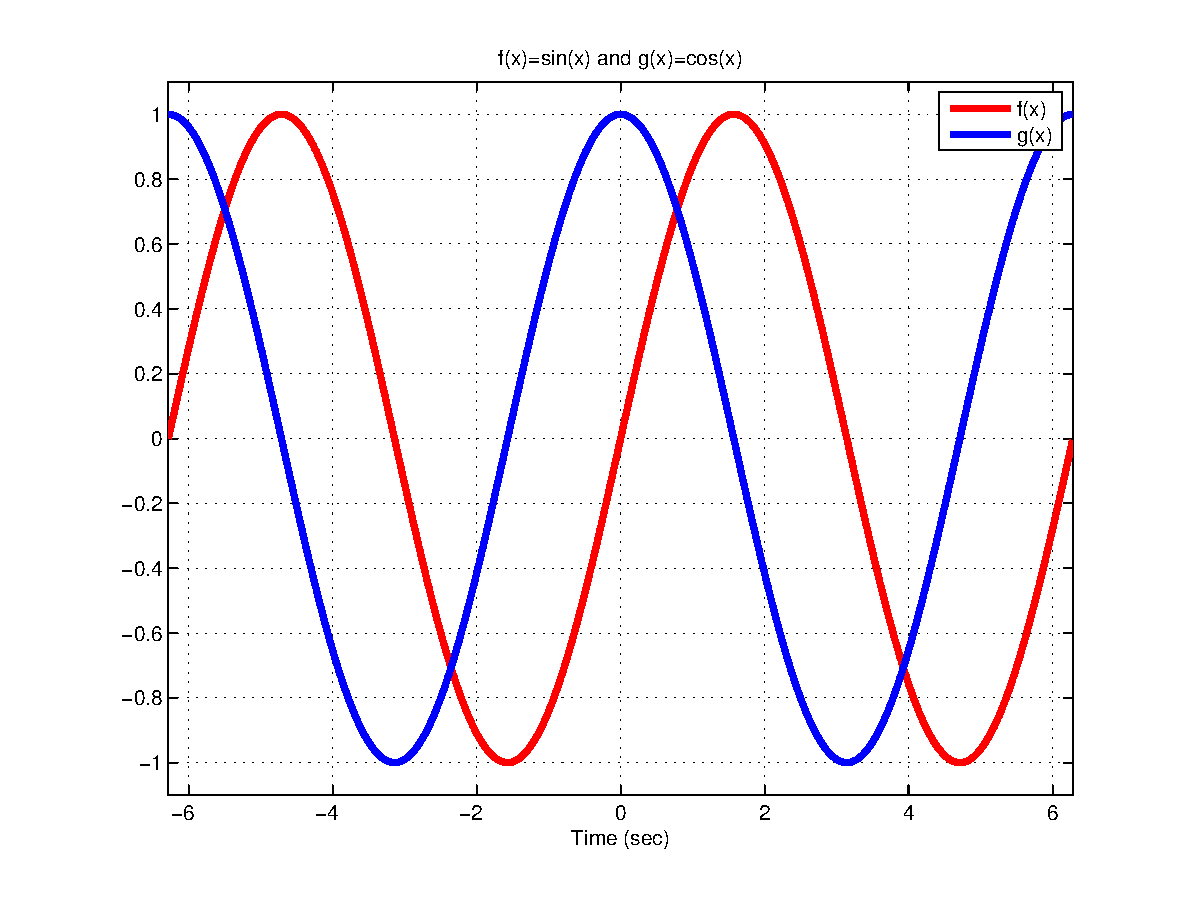
\includegraphics[width=0.7\columnwidth]{SampleFigure.eps}
    \caption{Figure for Example \ref{ex:C3:fig}
    \label{fig:C3:fig}
\end{figure}
\end{verbatim}
\end{example}
    \begin{figure}[ht!]
        \begin{center}
            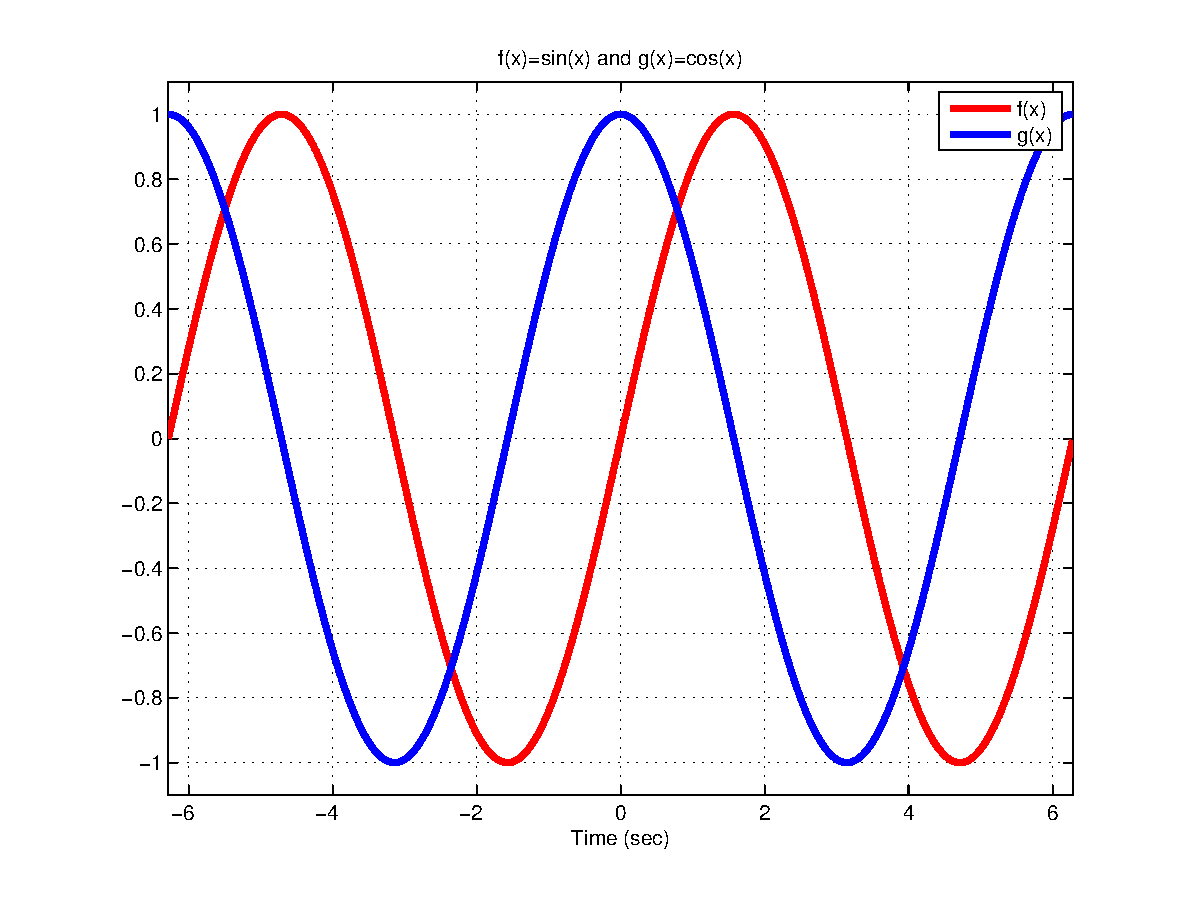
\includegraphics[width=0.7\columnwidth]{SampleFigure.eps}
        \end{center}
        \caption{Figure for Example \ref{ex:C3:fig}}
        \label{fig:C3:fig}
    \end{figure}



\subsection{New Commands: Shortcuts are AWESOME!}
You can save yourself a vast amount of typing by defining new commands which meet your
specific need. It is easy. The \texttt{newcommand} \index{newcommand} command goes in the preamble (before
the \verb|\begin{document}|). The examples that follow are a few handy ones that I've used
in the past.  The world is your oyster here, so make any shortcut for a \LaTeX\ command
that is cumbersome to type.
\begin{itemize}
    \item Derivatives
\begin{verbatim}
\newcommand{\dd}[2] {\frac{d #1}{d #2}}
\newcommand{\ddd}[2] {\frac{d^2 #1}{d #2^2}}

\dd{y}{x}
\ddd{y}{x}
\end{verbatim}

The results are:\\
\[\dd{y}{x}\]
\[\ddd{y}{x}\]

\item Partial derivatives
\begin{verbatim}
\newcommand{\pd}[2] {\frac{\partial{#1}}{\partial{#2}}}
\newcommand{\pdd}[2] {\frac{\partial^2{#1}}{\partial{#2}^2}}
\newcommand{\pddm}[3] {\frac{\partial^2{#1}}{\partial{#2}\partial{#3}}}

\pd{y}{x}
\pdd{y}{x}
\pddm{y}{x}{z}
\end{verbatim}

The results are:\\
\[\pd{y}{x}\]
\[\pdd{y}{x}\]
\[\pddm{y}{x}{z}\]

\item Some of the common number sets
\begin{verbatim}
\newcommand{\cc}{\mathbb{C}}
\newcommand{\rr}{\mathbb{R}}
\newcommand{\nn}{\mathbb{N}}
\newcommand{\qq}{\mathbb{Q}}
\newcommand{\zz}{\mathbb{Z}}

\cc \hspace{1cm} \nn \hspace{1cm} \qq \hspace{1cm} \rr \hspace{1cm} \zz
\end{verbatim}
The result is:
\[\cc \hspace{1cm} \nn \hspace{1cm} \qq \hspace{1cm} \rr \hspace{1cm} \zz\]

\item Grouping symbols (parentheses, brackets, etc) \index{grouping!parenthesis}
    \index{grouping!brackets}
\begin{verbatim}
\newcommand{\lp}{\left(}
\newcommand{\rp}{\right)}
\newcommand{\lb}{\left[}
\newcommand{\rb}{\right]}

\lp\pdd{F}{x}\rp
compared to
(\pdd{F}{x})
\end{verbatim}

The result is:
\[\lp\pdd{F}{x}\rp\]
compared to
\[(\pdd{F}{x})\]

\item Common conjunctions
\begin{verbatim}
\newcommand{\andd}[1]{\quad\text{and}\quad}
\newcommand{\orr}[1]{\quad\text{or}\quad}
\newcommand{\forr}[1]{\quad\text{for}\quad}
\newcommand{\st}[1]{\quad\text{such that}\quad}
\newcommand{\conj}[1]{\quad\text{#1}\quad}

% Implies
\newcommand{\ra}{\quad\Rightarrow\quad}

A\ra B\st C\ne D
\end{verbatim}

The result is:
\[A\ra B\st C\ne D\]
\end{itemize}



\section{Graphics in \LaTeX}
In this chapter we will focus on several tools that extend your knowledge of figures
beyond just \texttt{includegraphics} and move you toward the domain of professional
publications.  The tools that we'll cover are:\index{graphics!tikz}
\index{graphics!pgfplots} \index{graphics!GeoGebra}  \index{graphics!MatLab}
\begin{enumerate}
    \item The \texttt{tikz} package,
    \item The \texttt{pgfplots} package,
    \item Using \texttt{GeoGebra} to generate \texttt{tikz} code, and 
    \item Using \texttt{MatLab} to generate \texttt{tikz} code.
\end{enumerate}

These tools take a lot of work, but the end result is well worth it.  
\begin{center}
    {\bf There is nothing worse or more distracting than a poorly done figure.}
\end{center}

There is more to these packages than we could possibly cover in a few days.  It is
imperative that you use the internet to its fullest extent with these packages.  You can
get yourself into a pickle with some of the internet-based examples, but starting with someone
else's code for these packages is \"uber helpful sometimes!

What I'll present here are simply a few examples to get you going.

\subsection{The Tikz and PGFPlots Packages}
The Tikz package is made for doing line drawings.  The simplest mode of operation with
Tikz is to do point-by-point drawings on a Cartesian grid.
\begin{example}
    Say we want to draw a coordinate plane with a few geometric shapes.  Inside the
    \texttt{figure} environment we include a \texttt{tikzpicture} environment around the
    code for the picture.  Be sure to end every Tikz line with a semicolon;  Figure
    \ref{fig:C5:tikz1} shows the results. \index{graphics!draw}
    \index{graphics!tikzpicture}
\begin{verbatim}
\begin{tikzpicture}
    \draw[color=gray] (-3,-3) grid (3,3);
    \draw[thick, <->] (-3,0) -- (3,0) node[anchor=west]{$x$};
    \draw[thick, <->] (0,-3) -- (0,3) node[anchor=south]{$y$};
    \draw[very thick, blue, fill=blue!50] (0,0) -- 
        (2,1) -- (1,3) -- cycle;
    \draw[very thick, dashed, color=red, 
        fill=red!20!blue, opacity=0.5] (-2,0) circle(1cm);
\end{tikzpicture}
\end{verbatim}
\end{example}
    \begin{figure}[ht!]
        \begin{center}
            \begin{tikzpicture}
                \draw[color=gray] (-3,-3) grid (3,3);
                \draw[thick, <->] (-3,0) -- (3,0) node[anchor=west]{$x$};
                \draw[thick, <->] (0,-3) -- (0,3) node[anchor=south]{$y$};
                \draw[very thick, blue, fill=blue!50] (0,0) -- (2,1) -- (1,3) -- cycle;
                \draw[very thick, dashed, color=red, fill=red!20!blue, opacity=0.5] (-2,0) circle(1cm);
            \end{tikzpicture}
        \end{center}
        \caption{A simple Tikz picture}
        \label{fig:C5:tikz1}
    \end{figure}

For more examples about the Tikz package, see
\href{http://www.texample.net/tikz/examples/}{http://www.texample.net/tikz/examples/}
\dots texample \index{texample} is your new best friend.




You don't have to plot in MatLab, Excel, or any other tool when writing a technical
document!  Say this to yourself 100 times and be sure that you're sitting down.

\begin{example}
    This first example shows a simple way to plot functions. \index{graphics!axis}
    \index{graphics!addplot} \index{graphics!addlegendentry}
\begin{verbatim}
\begin{tikzpicture}
    \begin{axis}[axis lines=center, xlabel={x}, 
            title={My Awesome Plot},
            domain=-2*pi:2*pi, ymin=-1.5, ymax=2, grid]
        \addplot[blue, thick, smooth] {sin(deg(x))};
        \addlegendentry{$f(x)=\sin(x)$};
        \addplot[red, thick, smooth] {cos(deg(x))};
        \addlegendentry{$g(x)=\cos(x)$};
        \addplot[black, dashed, thick, smooth] {0.1*exp(-x)};
        \addlegendentry{$h(x)=0.1\text{exp}(-x)$};
    \end{axis}
\end{tikzpicture}
\end{verbatim}
\end{example}
    \begin{figure}[ht!]
        \begin{center}
            \begin{tikzpicture}
                \begin{axis}[axis lines=center, xlabel={x}, title={My Awesome Plot},
                    domain=-2*pi:2*pi, ymin=-1.5, ymax=2, grid]
                    \addplot[blue, thick, smooth] {sin(deg(x))};
                    \addlegendentry{$f(x)=\sin(x)$};
                    \addplot[red, thick, smooth] {cos(deg(x))};
                    \addlegendentry{$g(x)=\cos(x)$};
                    \addplot[black, dashed, thick, smooth] {0.1*exp(-x)};
                    \addlegendentry{$h(x)=0.1\text{exp}(-x)$};
                \end{axis}
            \end{tikzpicture}
        \end{center}
        \caption{A figure drawn with the \texttt{tikzpicture} and \texttt{axis} commands
        (leveraging the \texttt{pgfplots} package in the backgroud).}
        \label{fig:C5:pgf}
    \end{figure}

Next we'll follow with several more examples. Some of them are very advanced and some are
beautifully simple.

\begin{example}\label{ex:C5:bar}
Draw a bar chart for the following table of the world's largest producers of gem-quality
diamonds in 2010. The solution is shown in Figure \ref{fig:C5:bar}.
\begin{center}
\renewcommand{\arraystretch}{1.2}
\begin{tabular}{|c|c|} \hline
Country & Millions of Carats \\\hline
Botswana & 25.0 \\\hline
Russia & 17.8 \\\hline
Angola &12.5 \\\hline
Canada & 11.8 \\\hline
Congo & 5.5 \\\hline
\end{tabular}\end{center}
Souce: USGS Mineral Commodity Summaries.

\begin{verbatim}
\usetikzlibrary{patterns}
\pgfplotsset{width=12cm,height=8cm}
\begin{tikzpicture}
    \begin{axis}[
            ybar,
            bar width=10mm,
            enlargelimits=0.15,
            xlabel={\Large{Country}},
            ylabel={\Large{Millions of Carats}},
            title={\Large{World's Largest Diamond Producers 2010}},
            xtick=data,
            symbolic x coords={Botswana,Russia,Angola,Canada,Congo},
            nodes near coords,
            axis lines*=left
        ]
        \addplot [pattern=crosshatch dots,pattern color=red!80!white,
            draw=red] coordinates {(Botswana,25) 
            (Russia,17.8) (Angola,12.5) (Canada,11.8) (Congo,5.5)};
    \end{axis}
\end{tikzpicture}
\end{verbatim}
\end{example}
\usetikzlibrary{patterns}
\pgfplotsset{width=12cm,height=8cm}
\begin{figure}
    \begin{center}
        \begin{tikzpicture}
            \begin{axis}[
                    ybar,
                    bar width=10mm,
                    enlargelimits=0.15,
                    xlabel={\Large{Country}},
                    ylabel={\Large{Millions of Carats}},
                    title={\Large{World's Largest Diamond Producers 2010}},
                    xtick=data,
                    symbolic x coords={Botswana,Russia,Angola,Canada,Congo},
                    nodes near coords,
                    axis lines*=left
                ]
                \addplot [pattern=crosshatch dots,pattern color=red!80!white,draw=red] coordinates {(Botswana,25) (Russia,17.8) (Angola,12.5) (Canada,11.8) (Congo,5.5)};
            \end{axis}
        \end{tikzpicture}
    \end{center}
    \caption{Figure for Example \ref{ex:C5:bar}}
    \label{fig:C5:bar}
\end{figure}


\section{Bibliography Management}
There are two primary ways to manage a bibliography file in \LaTeX.  In both ways you need
to remember that (as usual) you have full control over everything!  Two rules of thumb:
\begin{enumerate}
    \item If you are using a short bibliography or if this paper stands alone then you
        probably want to use an embedded bibliography.
    \item If you have a collection of references that will be used for several papers then
        you should consider using a BibTeX database.
\end{enumerate}
Both types of bibliographies will save huge amounts of time and allow for very simple
citation formats. 

As usual, there is MUCH more to writing a good bibliography than what can possibly be
listed here.  A really good source is the wiki page for the latex bibliography: \\
\href{http://en.wikibooks.org/wiki/LaTeX/Bibliography_Management}{http://en.wikibooks.org/wiki/LaTeX/Bibliography\_Management}.

\subsection{Embedded Bibliography}\index{bibliography!embedded}
If you're using an embedded bib for a stand-alone paper then just before the
\verb|\end{document}| you include all of the bibliography information.  A simple example
(with 1 paper) is included here:
\begin{verbatim}
\begin{thebibliography}{9}

\bibitem{lamport94}
  Leslie Lamport,
  \emph{\LaTeX: a document preparation system},
  Addison Wesley, Massachusetts,
  2nd edition,
  1994.

\end{thebibliography}
\end{verbatim}

Use the \verb|\cite{ }| \index{bibliography!cite} command to cite items that are listed
labeled inside the curly braces after \verb|\bibitem|. \index{bibliography!bibitem}  For
example, if we type \verb|\cite{lamport94}| then we get a citation like this:
\cite{lamport94}.


\subsection{Bibliography Database: BibTeX}\index{bibliography!database|see {bibtex}}
BibTeX is a way for you to keep all of your bibliography materials in one place.  The
basic idea is as follows: \index{bibliography!bibtex}
\begin{enumerate}
    \item Start a file called \texttt{MyBib.bib} and follow the instructions from the link
        below to build your bibliography:\\
        \href{http://ccm.ucdenver.edu/wiki/How_to_write_BibTeX_files}{http://ccm.ucdenver.edu/wiki/How\_to\_write\_BibTeX\_files}
    \item In your \LaTeX\ file you can cite bib items with the \verb|\cite{ }| command.
        \index{bibliography!cite}  As you cite works and compile you will build the
        bibliography automatically.  You will need to compile MANY times to get all of the
        cross referencing and citations to appear.
    \item Be sure that the \texttt{*.bib} file is in the same working directory as your
        \LaTeX\ document (or at least give a path).
\end{enumerate}

The primary utility of a bibtex file is that you can simply build it once when you're
working on a large project and the citations will draw only the parts that are necessary
for the current paper.  





\chapter{Optional Material}

\newpage\section{Low Rank Approximations of Matrices}

\begin{problem}
    One particular use of the SVD is for data reduction.  The word ``reduction'' here
    really means that we are going to make approximations of data using lower dimensions,
    and a very visually stunning way to do this is to do data reduction on images.  The following code will read
    the file \mcode{TestImage.jpg} into MATLAB and convert it to a rectangular matrix of
    values.  It is up to the reader to supply the necessary image.
\begin{lstlisting}
A = imread('TestImage.jpg');
A = A(:,:,1);
A = im2double(A);
imshow(A)
\end{lstlisting}
    Once the matrix is in MATLAB do the following.  In this we assume that $A$ is an $m
    \times n$ matrix.
    \begin{enumerate}
        \item Find the SVD of the image (remember the semicolons!!!!!!).  This will take
            over a minute with our code so be patient.  Once it is done check that your
            SVD code does a decent approximation of the original image.
\begin{lstlisting}
[U,S,V] = MySVD(A);
error = norm(A - U*S*V')
\end{lstlisting}
        \item Get the singular values out of $\Sigma$ and find the largest $P$\% of the
            singular values. Let's say that this is $N$ values.  Create four new matrices
            $U_{new}$, $\Sigma_{new}$, $V_{new}$, and $A_{new}$ in the following way.
            \begin{enumerate}
                \item $U_{new}$ is $m \times N$ and contains only the first $N$ columns of
                    $U$.
                \item $\Sigma_{new}$ is $N \times N$ and contains only the top $P$\% of
                    the singular values of $A$.
                \item $V_{new}$ is $n \times N$ and contains the first $N$ columns of $V$.
                \item $A_{new}$ is $m \times n$ and is formed by $U_{new} \Sigma_{new}
                    V_{new}^T$.  
            \end{enumerate}
        \item Show the newly data-reduced image with \\
            \mcode{imshow(Anew)}
        \item The rank of the new image is equal to the number of singular values that you
            kept in step 2.  
        \item Experiment with several low rank approximations of an image starting with
            rank 1 and progress up to larger and larger ranks matrices.  You'll find that
            the rank necessary to recover the full image is much lower than than the full
            original rank.
    \end{enumerate}
\end{problem}


\newpage\section{The Google Page Rank Algorithm}
In this section you will discover how the PageRank algorithm works to give the most relevant
information as the top hit on a Google search.  

Search engines compile large indexes of the dynamic information on the Internet so they
are easily searched.  This means that when you do a Google search, you are not actually
searching the Internet; instead, you are searching the indexes at Google.

When you type a query into Google the following two steps take place:
\begin{enumerate}
    \item Query Module: The query module at Google converts your natural language into a
        language that the search system can understand and consults the various indexes
        at Google in order to answer the query.  This is done to find the list of relevant
        pages.
    \item Ranking Module: The ranking module takes the set of relevant pages and ranks
        them. The outcome of the ranking is an ordered list of web pages such
        that the pages near the top of the list are most likely to be what you desire from
        your search. This ranking is the same as assigning a {\it popularity score} to
        each web site and then listing the relevant sites by this score.  
\end{enumerate}

This section focuses on the Linear Algebra behind the Ranking Module developed by the
founders of Google: Sergey Brin and Larry Page.  Their algorithm is called the
\emph{PageRank algorithm}, and you use it every single time you use Google's search
engine.


In simple terms: {\it A webpage is important if it is pointed to by other important
pages}.

The Internet can be viewed as a directed graph (look up this term
\href{https://en.wikipedia.org/wiki/Directed_graph}{here on Wikipedia}) where the nodes
are the web pages and the edges are the hyperlinks between the pages. The hyperlinks into a
page are called {\it inlinks}, and the ones pointing out of a page are called {\it
outlinks}.  In essence, a hyperlink from my page to yours is my endorsement of your page.
Thus, a page with more recommendations must be more important than a page with a few
links.  However, the status of the recommendation is also important. 

Let us now translate this into mathematics. To help understand
this we first consider the small web of six pages shown in Figure
\ref{fig:example_graph} (a graph of the router level of the internet can be found
\href{https://personalpages.manchester.ac.uk/staff/m.dodge/cybergeography/atlas/lumeta_large.jpg}{here}).  The links between the
pages are shown by arrows. An arrow pointing into a node is an {\it inlink}
and an arrow pointing out of a node is an {\it outlink}. In Figure
\ref{fig:example_graph}, node 3 has three outlinks (to nodes 1, 2, and 5)
and 1 inlink (from node 1).

\begin{figure}[ht]
    \begin{center}
        \begin{tikzpicture}
            \draw (0,0) node[circle,draw]{3};
            \draw (-1,1) node[circle,draw]{1};
            \draw (1,1) node[circle,draw]{2};
            \draw (-1,-1) node[circle,draw]{6};
            \draw (1,-1) node[circle,draw]{5};
            \draw (0,-2) node[circle,draw]{4};
        %
            \draw[<->] (-0.25,0.25) -- (-0.75,0.75);
            \draw[->] (-0.65,1) -- (0.65,1);
            \draw[->] (0.25,0.25) -- (0.75,0.75);
            \draw[->] (0.25,-0.25) -- (0.75,-0.75);
            \draw[->] (0.65,-1) -- (-0.65,-1);
            \draw[<->] (-0.75,-1.25) -- (-.25,-1.75);
            \draw[<->] (0.75,-1.25) -- (0.25,-1.75);
        \end{tikzpicture}
    \end{center}
        \caption{Sample graph of a web with six pages.}
        \label{fig:example_graph}
\end{figure}

We will first define some notation in the PageRank algorithm:
\begin{itemize}
    \item $|P_i|$ is the number of outlinks from page $P_i$
    \item $H$ is the {\it hyperlink} matrix defined as 
        \[ H_{ij} = \left\{ \begin{array}{cl} \frac{1}{|P_j|}, & \text{if there is a link
            from node $j$ to node $i$} \\ 0, & \text{otherwise} \end{array} \right. \]
        where the ``$i$'' and ``$j$'' are the row and column indices respectively.  
    \item $\bx$ is a vector that contains all of the PageRanks for the individual pages.
\end{itemize}

The PageRank algorithm works as follows:
\begin{enumerate}
    \item Initialize the page ranks to all be equal. This means that our initial
        assumption is that all pages are of equal rank.  In the case of Figure
        \ref{fig:example_graph} we would take $\bx_0$ to be 
        \[ \bx_0 = \begin{pmatrix} 1/6 \\ 1/6 \\ 1/6 \\ 1/6 \\ 1/6 \\ 1/6 \end{pmatrix}. \]
    \item Build the hyperlink matrix.  \\ As an example we'll consider node 3 in Figure
        \ref{fig:example_graph}.  There are three outlinks from node 3 (to nodes 1, 2, and
        5).  Hence $H_{13}=1/3$, $H_{23} = 1/3$, and $H_{53} = 1/3$ and the partially
        complete hyperlink matrix is
        \[ H = \begin{pmatrix} 
                - & - & 1/3 & - & - & - \\
                - & - & 1/3 & - & - & - \\
                - & - & 0   & - & - & - \\
                - & - & 0   & - & - & - \\
                - & - & 1/3 & - & - & - \\
                - & - & 0   & - & - & - 
            \end{pmatrix} \]
    \item The difference equation $\bx_{n+1} = H \bx_n$ is used to iteratively refine the
        estimates of the page ranks.  You can view the iterations as a person visiting a
        page and then following a link at random, then following a random link on the next
        page, and the next, and the next, etc.  Hence we see
        that the iterations evolve exactly as expected for a difference equation.
        \begin{center}
            \begin{tabular}{|c|c|}
                \hline
                Iteration & New Page Rank Estimation \\ \hline \hline
                0 & $\bx_0$ \\
                1 & $\bx_1 = H \bx_0$ \\
                2 & $\bx_2 = H \bx_1 = H^2 \bx_0$ \\
                3 & $\bx_3 = H \bx_2 = H^3 \bx_0$ \\
                4 & $\bx_4 = H \bx_3 = H^4 \bx_0$ \\
                \vdots & \qquad \vdots \\
                $k$ & $\bx_k = H^k \bx_0$ \\ \hline
            \end{tabular}
        \end{center}
    \item When a steady state is reached we sort the resulting vector $\bx_k$ to give the
        page rank. The node (web page) with the highest rank will be the top search
        result, the second highest rank will be the second search result, and so on.
\end{enumerate}

It doesn't take much to see that this process can be very time consuming.  Think about
your typical web search with hundreds of thousands of hits; that makes a square matrix $H$
that has a size of hundreds of thousands of entries by hundreds of thousands of entries!
The matrix multiplications alone would take many minutes (or possibly many hours) for
every search! \dots but Brin and Page were pretty smart dudes!!


We now state a few theorems and definitions that will help us simplify the iterative
PageRank process.
\begin{thm}\label{thm:eigen_expand}
    If $A$ is an $n \times n$ matrix with $n$ linearly independent eigenvectors $\bv_1,
    \bv_2, \bv_3,$ $\ldots, \bv_n$ and associated eigenvalues $\lambda_1, \lambda_2,
    \lambda_3, \ldots, \lambda_n$ then for any initial vector $\bx \in \mathbb{R}^n$ we
    can write $A^k \bx$ as
    \[ A^k \bx = c_1 \lambda_1^k \bv_1 + c_2 \lambda_2^k \bv_2 + c_3 \lambda_3^k \bv_3 +
        \cdots c_n \lambda_n^k \bv_n \]
    where $c_1, c_2, c_3, \ldots, c_n$ are the constants found by expressing $\bx$ as a
    linear combination of the eigenvectors. \\Note: We can assume that the eigenvalues are ordered
    such that $\lambda_1 \ge \lambda_2 \ge \lambda_3 \ge \cdots \ge \lambda_n$.
\end{thm}
\begin{proof}
    (Prove the preceding theorem)
\end{proof}

\begin{definition}
    A {\bf probability vector} is a vector with entries on the interval $[0,1]$ that add up to 1. 
\end{definition}
\begin{definition}
    A {\bf stochastic matrix} is a square matrix whose columns are probability vectors.
\end{definition}

\begin{thm} \label{thm:largest_ev_stochastic}
    If $A$ is a stochastic $n \times n$ matrix then $A$ will have $n$ linearly independent
    eigenvectors.  Furthermore, the largest eigenvalue of a stochastic matrix will
    \underline{always} be $\lambda_1 = 1$ and the smallest eigenvalue  will always be
    nonnegative: $0 \le \lambda_n < 1$.
\end{thm}

Some of the following tasks will ask you to {\it prove} a statement or a theorem.  This
means to clearly write all of the logical and mathematical reasons why the statement is
true. Your proof should be absolutely crystal clear to anyone with a similar mathematical
background \dots if you are in doubt then have a peer from a different group read your
proof to you \underline{out loud}.

\begin{problem}
    Finish writing the hyperlink matrix $H$ from Figure \ref{fig:example_graph}.
\end{problem}

\begin{problem}
    Write MATLAB code to implement the iterative process defined previously. Make a plot
    that shows how the rank evolves over the iterations.
\end{problem}


\begin{problem}
    What must be true about a collection of $n$ pages such that an $n\times n$
        hyperlink matrix $H$ is a stochastic matrix.
\end{problem}

The statement of the next theorem is incomplete, but the proof is given to you.  Fill in
the blank in the statement of the theorem and provide a few sentences supporting your
answer.
\begin{thm}\label{thm:steady}
    If $A$ is an $n \times n$ stochastic matrix and $\bx_0$ is some initial vector
    for the difference equation $\bx_{n+1} = A \bx_n$, then the steady state
    vector is
    \[ \bx_{equilib} = \lim_{k \to\infty} A^k \bx_0 = \underline{\hspace{1in}}. \]
\end{thm}
\begin{proof}
    First note that $A$ is an $n \times n$ stochastic matrix so from Theorem
    \ref{thm:largest_ev_stochastic} we know that there are $n$ linearly
    independent eigenvectors.  We can then substitute
    the eigenvalues from Theorem \ref{thm:largest_ev_stochastic} in Theorem
    \ref{thm:eigen_expand}. Noting that if $0<\lambda_j<1$ we have $\lim_{k \to
    \infty} \lambda_j^k = 0$ the result follows immediately.
\end{proof}
\begin{problem}
    Discuss how Theorem \ref{thm:steady} greatly simplifies the PageRank iterative process
    described previously.  In other words: there is no reason to iterate at all.  Instead,
    just find \underline{\hspace{1in}}.
\end{problem}
\begin{problem}
\item Now use the previous two problems to find the resulting PageRank vector from the web in Figure
    \ref{fig:example_graph}?  Be sure to rank the pages in order of importance.
    Compare your answer to the one that you got in problem 2.
\end{problem}


\begin{problem}
    Consider the web in Figure \ref{fig:graph2}.
        \begin{enumerate}
            \item[(a)] Write the $H$ matrix and find the initial state $\bx_0$, 
            \item[(b)] Find
                steady state PageRank vector using the two different methods described:
                one using the iterative difference equation and the other using Theorem
                \ref{thm:steady} and the dominant eigenvector.
            \item[(c)] Rank the pages in order of importance.
        \end{enumerate}
\end{problem}
\begin{figure}[ht!]
    \begin{center}
        \begin{tikzpicture}
            \draw (0,0) node[circle,draw]{3};
            \draw (-1,1) node[circle,draw]{1};
            \draw (1,1) node[circle,draw]{2};
            \draw (-1,-1) node[circle,draw]{6};
            \draw (1,-1) node[circle,draw]{5};
            \draw (0,-2) node[circle,draw]{4};
            \draw (-2,0) node[circle,draw]{7};
            \draw (-2,-2) node[circle,draw]{8};
        %
            \draw[<-] (-0.25,0.25) -- (-0.75,0.75);
            \draw[->] (-0.65,1) -- (0.65,1);
            \draw[<->] (0.25,0.25) -- (0.75,0.75);
            \draw[<->] (0.25,-0.25) -- (0.75,-0.75);
            \draw[->] (0.65,-1) -- (-0.65,-1);
            \draw[<->] (-0.75,-1.25) -- (-.25,-1.75);
            \draw[<->] (0.75,-1.25) -- (0.25,-1.75);
            \draw[<->] (-1.75,0.25) -- (-1.25,0.75);
            \draw[<->] (-1.65,0) -- (-0.35,0);
            \draw[<-] (-1.75,-0.25) -- (0.7,-0.8);
            \draw[->] (-2,-0.35) -- (-2,-1.65);
            \draw[<->] (-1.65,-2) -- (-0.35,-2);
        \end{tikzpicture}
    \end{center}
    \caption{Graph of a web with eight pages.}
    \label{fig:graph2}
\end{figure}


\begin{problem}
    One thing that we didn't consider in this version of the Google Page Rank algorithm is
    the random behavior of humans.  One, admittedly slightly naive, modification that we
    can make to the present algorithm is to assume that the person surfing the web will
    randomly jump to any other page in the web at any time.  For example, if someone is on
    page 1 in Figure \ref{fig:graph2} then they could randomly jump to any page 2 - 8.
    They also have links to pages 2, 3, and 7.  That is a total of 10 possible next steps
    for the web surfer.  There is a $2/10$ chance of heading to page 2.  One of those is
    following the link from page 1 to page 2 and the other is a random jump to page 2
    without following the link.  Similarly, there is a $2/10$ chance of
    heading to page 3, $2/10$ chance of heading to page 7, and a $1/10$ chance of randomly
    heading to any other page.

    Implement this new algorithm, called the {\it random surfer algorithm}, on the web in
    Figure \ref{fig:graph2}.  Compare your ranking to the non-random surfer results from
    the previous problem.
\end{problem}



\newpage\section{Principal Component Analysis (Incomplete)}

\newpage\section{Building PDE's From Conservation Laws}

In this section
we'll give a more analytic introduction to most of the primary partial
differential equations of interest in basic mathematical physics.  We will make reference
to Fick's Law for mass transport and Fourier's Law for thermal transport, so interested
readers should dig deeper by examining the relevant Wikipedia pages or other sources.
  
Conservation laws pervade all of physics -- conservation of energy, conservation of
momentum, and conservation of mass.  These laws are sometimes stated colloquially as
{\it energy (or momentum or mass) can neither be created nor destroyed}, but this phrase
is not super helpful mathematically.  We start this section with a brief mathematical
derivation of a {\it general conservation law} to further clarify what we mean
mathematically.  The resulting general conservation law will be a
partial differential equation that can be used to mathematically express the physical laws
of conservation of mass, momentum, or
energy.

Let $u$ be the quantity you are trying to conserve, $\bq$ be the flux of that quantity,
and $f$ be any source of that quantity.  For example, if we are to derive a conservation
of energy equation, $u$ might be energy, $\bq$ might be temperature flux, and $f$ might be
a temperature source (or sink).

\subsection*{Derivation of General Balance Law}
Let $\Omega$ be a fixed volume and denote the boundary of this volume by $\partial
\Omega$. The rate at which $u$ is changing in time throughout $\Omega$ needs to be
balanced by the rate at which $u$ leaves the volume plus any sources of $u$.
Mathematically, this means that
\begin{flalign}
    \pd{ }{t} \iiint_{\Omega} u dV = -\iint_{\partial \Omega} \bq \cdot n dA +
    \iiint_\Omega f dV.
    \label{eqn:global_balance}
\end{flalign}
This is a global balance law in the sense that it holds for all volumes $\Omega$.  The
mathematical 
troubles here are two fold: (1) there are many integrals, and (2) there are really two variables
($u$ and $q$ since $f=f(u,x,t)$) so the equation is not closed.  In order to mitigate
that fact we apply the divergence theorem to the first term on the right-hand side of
\eqref{eqn:global_balance} to get
\begin{flalign}
    \pd{ }{t} \iiint_{\Omega} u dV = -\iiint_{\Omega} \nabla \cdot \bq dV +
    \iiint_\Omega f dV.
    \label{eqn:global_balance2}
\end{flalign}

Gathering all of the terms on the right of \eqref{eqn:global_balance2}, interchanging the integral and the derivative on
the left (since the volume is not changing in time), and rewriting gives
\begin{flalign}
    \iiint_\Omega \left( \pd{u}{t} + \nabla \cdot \bq \right) dV = \iiint_\Omega f dV
    \label{eqn:global_balance3}
\end{flalign}
If we presume that this equation holds for all volumes $\Omega$ then the integrands must
be equal and we get the local balance law
\begin{flalign}
    \pd{u}{t} + \nabla \cdot \bq = f.
    \label{eqn:local_balance}
\end{flalign}

Equation \eqref{eqn:local_balance} is an expression of the balances of changes in time to
changes in space of a conserved quantity such as mass, momentum, or energy.  What remains
is to make clear the meaning and functional form of the flux $\bq$ and the source function
$f$.

\subsection*{Simplification of the Local Balance Law}
In equation \eqref{eqn:local_balance} it is often assumed that the system is free of
external sources.  In this case we set $f$ to zero and obtain the source-free balance law
\begin{flalign}
    \pd{u}{t} + \nabla \cdot \bq = 0.
    \label{eqn:local_source_free}
\end{flalign}
It is this form of balance law where many of the most interesting and important partial
differential equations come from.  In particular consider the following two cases: mass
balance and energy balance.
\subsection*{Mass Balance}
In mass balance we take $u$ to either be the density of a substance (e.g. in the case of
liquids) or the concentration of a substance in a mixture (e.g. in the case of
gasses). If $C$ is the mass concentration of a substance in a gas then the flux of that
substance is given via Fick's Law as
\begin{flalign}
    \bq = -k \nabla C.
    \label{eqn:fick}
\end{flalign}
Combining \eqref{eqn:fick} with \eqref{eqn:local_source_free} (and assuming that $k$ is
independent of space, time, and concentration) gives
\begin{flalign}
    \pd{C}{t} = k \nabla \cdot \nabla C. 
    \label{eqn:fick2_simp}
\end{flalign}
In the presence of external sources of mass, \eqref{eqn:fick2_simp} is
\begin{flalign}
    \pd{C}{t} = k \nabla \cdot \nabla C + f(x).
    \label{eqn:fick3}
\end{flalign}
Expanding the Laplacian operator on the right-hand side of \eqref{eqn:fick3} we get
\begin{flalign}
    \pd{C}{t} = k\left( \pdd{C}{x} + \pdd{C}{y} + \pdd{C}{z} \right) + f(x)
    \label{eqn:fick3_expanded}
\end{flalign}
where the reader should note that this can be easily simplified in 1 or 2 spatial
dimensions.
% \begin{problem}
%     What does \eqref{eqn:fick3} equation look like in terms of spatial derivatives on the
%     right-hand side?
%     \begin{flalign*}
%         \pd{C}{t} &= \underline{\hspace{2in}} \quad \text{(1 Spatial Dimension)} \\
%         \pd{C}{t} &= \underline{\hspace{2in}} \quad \text{(2 Spatial Dimensions)} \\
%         \pd{C}{t} &= \underline{\hspace{2in}} \quad \text{(3 Spatial Dimensions)}
%     \end{flalign*}
% \end{problem}

\subsection*{Energy Balance}
The energy balance equation is essentially the same as the mass balance equation.  If $u$
is temperature then the flux of temperature is given by Fourier's Law for heat conduction
\begin{flalign}
    \bq = -k\nabla T.
    \label{eqn:fourier}
\end{flalign}
Making the same simplifications as in the mass balance equation we arrive at
\begin{flalign}
    \pd{T}{t} = k \nabla \cdot \nabla T.
    \label{eqn:fourier2}
\end{flalign}
In the presence of external sources of heat, \eqref{eqn:fourier2} becomes
\begin{flalign}
    \pd{T}{t} = k \nabla \cdot \nabla T + f(x).
    \label{eqn:fourier3}
\end{flalign}
Expanding the Laplacian operator on the right-hand side of \eqref{eqn:fourier3} we get
\begin{flalign}
    \pd{T}{t} = k\left( \pdd{T}{x} + \pdd{T}{y} + \pdd{T}{z} \right) + f(x)
    \label{eqn:fourier3_expanded}
\end{flalign}
where the reader should note that this can be easily simplified in 1 or 2 spatial
dimensions.
% \begin{problem}
%     What does \eqref{eqn:fourier3} equation look like in terms of spatial derivatives on the
%     right-hand side?
%     \begin{flalign*}
%         \pd{T}{t} &= \underline{\hspace{2in}} \quad \text{(1 Spatial Dimension)} \\
%         \pd{T}{t} &= \underline{\hspace{2in}} \quad \text{(2 Spatial Dimensions)}\\
%         \pd{T}{t} &= \underline{\hspace{2in}} \quad \text{(3 Spatial Dimensions)}
%     \end{flalign*}
% \end{problem}



\subsection*{Laplace's Equation and Poisson's Equation}
Equations \eqref{eqn:fick3} and \eqref{eqn:fourier3} are the same partial differential
equation for two very important physical phenomenon; mass and heat transfer.  In the case
where time is allowed to run to infinity and no external sources of mass or energy are
included these equations reach a steady state solution (no longer changing in time) and we
arrive at Laplace's Equation
\begin{flalign}
    \nabla \cdot \nabla u = 0.
    \label{eqn:laplace}
\end{flalign}
Laplace's equation is actually a statement of minimal energy as well as steady state heat
or temperature.  We can see this since entropy always drives systems from high energy to
low energy, and if we have reached a steady state then we must have also reached a surface
of minimal energy.

Equation \eqref{eqn:laplace} is sometimes denoted as $\nabla \cdot \nabla u = \nabla^2 u =
\Delta u$, and in terms of the partial derivatives it is written as
\begin{flalign*}
    \pdd{u}{x} + \pdd{u}{y} + \pdd{u}{z} = 0.
% V    0 &= \underline{\hspace{2in}} \quad \text{(1 Spatial Dimension)} \\
%     0 &= \underline{\hspace{2in}} \quad \text{(2 Spatial Dimensions)} \\
%     0 &= \underline{\hspace{2in}} \quad \text{(3 Spatial Dimensions)} 
\end{flalign*}

If there is a time-independent external source the right-hand side of
\eqref{eqn:laplace} will be non-zero and we arrive at Poisson's equation:
\begin{flalign}
    \nabla \cdot \nabla u = -f(x).
    \label{eqn:poisson}
\end{flalign}
Note that the negative on the right-hand side comes from the fact that
$\pd{u}{t} = k \nabla \cdot \nabla u + f(x)$ and $\pd{u}{t} \to 0$.  Technically we are
absorbing the constant $k$ into $f$ (that is ``$f$'' is really ``$f/k$'').  Also
note that in many instances the value of $k$ is not constant and cannot therefore be pulled
out of the derivative without a use of the product rule.

Let's summarize:
\begin{center}
    \begin{tabular}{|c|c|c|}
        \hline
        Name of PDE & PDE & What the PDE Models \\ \hline \hline
        The Heat Equation & $\ds \pd{u}{t} = k \nabla \cdot \nabla u + f(x)$ & Diffusion \\
        Laplace's Equation & $\ds k \nabla \cdot \nabla u =-f(x)$ & Minimal Energy
        Surfaces \\
%         The Wave Equation & $\ds \pdd{u}{t} = k \nabla \cdot \nabla u + f(x)$ & Wave
%         phenomena \\
        \hline
    \end{tabular}
\end{center}

Further discussion of the origins of the wave equation and other interesting PDE's is left
to the reader.




\addcontentsline{toc}{chapter}{Bibliography}
\begin{thebibliography}{99}
        \bibitem{Chartier} A. Greenbaum and T. Charier. {\it Numerical Methods: Design,
            Analysis, and Computer Implementation of Algorithms} Princeton University
            Press. 2012.
        \bibitem{Burden} R. Burden, D, Faires, and A. Burden. {\it Numerical Analysis,
            10ed} Cengage Learning. 2016.
        \bibitem{Kincaid} D. Kindaid and W. Cheney. {\it Numerical Analysis, 2ed.}
            Brooks/Cole Publishing, 1996.
        \bibitem{Haberman} R. Haberman. {\it Applied Partial Differential Equations,
        4ed}.  Pearson Education Inc. Upper Saddle River, New Jersey, 2004
        \bibitem{Lay} D. Lay. {\it Linear Algebra 4ed.} Pearson Education Inc. Upper
        Saddle River, New Jersey, 2012.
        \bibitem{Meerschaert} M. Meerschaert. {\it Mathematical Modeling 4ed.} Academic
        Press Publications, 2013.
        \bibitem{Holistic} Holistic Numerical Methods
        \href{http://nm.mathforcollege.com/}{http://nm.mathforcollege.com/}\\
        The Holistic Numerical Methods book is probably the most complete free reference
        that I've found on the web.  This should be your source to look up deeper
        explanations of problems, algorithms, and code.
        \bibitem{SciCompMATLAB} Scientific Computing with MATLAB
        \href{http://gribblelab.org/scicomp/scicomp.pdf}{http://gribblelab.org/scicomp/scicomp.pdf}
        \bibitem{TeaTimeNumerical} Tea Time Numerical Analysis
        \href{http://lqbrin.github.io/tea-time-numerical/}{http://lqbrin.github.io/tea-time-numerical/}
\end{thebibliography}
\end{appendix}

\end{document}
%%%%%%%%%%%%%%%%%%%%%%%%%%%%%%%%%%%%%%%%%%%%%%%%%%%%%%%%%%%%%%%%%



